\documentclass[final,number,sort&compress,5p,times,twocolumn]{elsarticle}
%\documentclass[review,number,3p,times,sort&compress]{elsarticle}


\usepackage{lineno}
\linenumbers
\journal{Nucl.\ Instr.\ and Meth.\ A}

\usepackage{color} \newcommand{\red}[1]{\textcolor{red}{#1}}
\usepackage{subcaption}
\usepackage{wasysym}
\usepackage{graphicx}
\usepackage{hyperref}
\bibliographystyle{unsrt}
%\bibliographystyle{plainnat}
%\bibliographystyle{elsarticle-harv}




\usepackage{url}

\begin{document}
\begin{frontmatter}


\title{Texas Active Target (TexAT)}
    
 \author[Cyclotron]{E.~Koshchiy}
 \ead{koshchiy@tamu.edu}
  
 \author[Cyclotron,TAMU] {G.V.~Rogachev}
 \ead{rogachev@tamu.edu}
 
 \author[IRFU]{E.~Pollacco}

 \author[Cyclotron]{S.~Ahn}
 
 \author[Cyclotron]{E.~Uberseder}
 
 \author[Cyclotron]{ J.~Hooker} 
 
 \author[Cyclotron,TAMU]{J.~Bishop}
 
 \author[Cyclotron]{V.Z.~Goldberg}
 
 \author[Cyclotron]{M.~Barbui}
 
 \author[Cyclotron]{A.~Saastamoinen}
 
 \author[Cyclotron]{B.T.~Roeder}
 
 \author[Cyclotron]{C.~Magana}
 
 \author[Cyclotron]{C.H.~Hunt}
  
 \author[Cyclotron]{S.~Upadhiayula}

 \author[Cyclotron]{E.~Aboud}
 
 \author[Cyclotron]{H.~Jayatissa}
 
 \author[Cyclotron,TAMU]{R.~O'Dwyer}

  \address[Cyclotron]{Cyclotron Institute, Texas A\&M University, College Station, TX 77843, USA}
  
  \address[TAMU]{Department of Physics \& Astronomy, Texas A\&M University, College Station, TX 77843, USA}
  
  \address[IRFU]{IRFU, CEA, Saclay, Gif-Sur-Ivette, France}

 
  \begin{abstract}
  
The TexAT (Texas Active Target) detector is a new active-target time projection chamber (TPC) that was built at the Cyclotron Institute Texas A$\&$M University. The detector is designed to be of  general use for nuclear structure and nuclear astrophysics experiments with rare isotope beams. TexAT combines a highly segmented Time Projection  Chamber (TPC) with two layers of solid state detectors. It provides high efficiency and flexibility for experiments with low intensity exotic beams, allowing for the 3D track reconstruction of the incoming and outgoing particles involved in nuclear reactions and decays.

PACS 29.40.Cs Gas-filled counters: ionization chambers, proportional, and avalanche counters; 29.40.Gx Tracking and position-sensitive detectors

\begin{keyword}
    Active gas target;  Inverse kinematic; Time projection chambers;  Charge particles detection; Micromegas detector;
    Silicon-strip detectors; CsI(Tl)  detectors; Radioactive beams; Particle track; Vertex reconstruction
\end{keyword}


\end{abstract}
\end{frontmatter}

\section{Introduction}

Over the last 20-30 years experiments with rare isotope beams (RIBs) developed from being
exotic undertakings in select few laboratories into the main stream of nuclear science. RIBs provide a
pathway to venture far beyond the constrains typically encountered in the experiments with stable beams.
RIBs open up an opportunity to study very exotic nuclei using relatively simple and well understood
reactions, such as elastic and inelastic scattering, one/two nucleon transfer, Coulomb excitation, etc. They
allow to measure the key reaction rates that are relevant for explosive processes in astrophysics with
radioactive nuclei. All these benefits come at a price. Typical intensity of RIBs is many orders of
magnitude lower than intensity of stable beams. Therefore, efficiency of experimental setup becomes
determining factor for RIBs experiments. One of the most efficient experimental approach that can be
used with RIBs is active target detector. These detectors can be designed to have almost 4 $\pi$  solid angle
coverage, and they naturally allow to use thick target without loss of energy resolution. Thick target also
allows to measure reaction excitation functions without need to change the beam energy \cite{Goldberg} . The versatility
of these devises for RIBs experiments has been recognized and many nuclear physics laboratories around
the world are in the process of constructing and using these devices (TACTIC at U of York/TRIUMF \cite{TACTIC},
MAYA at GANIL/TRIUMF \cite{MAYA}, AT-TPC at NSCL \cite{AT-TPC}, ACTAR at GANIL/GSI \cite{ACTAR}, ANASEN  at
FSU/LSU/NSCL \cite{ANASEN}, and others). The comprehensive overeview on the subject  can be found in \cite{TPC_Review}, or  \cite{Ayyad2018}.
While the concept is similar for all active target detectors (the target material is spatially extended and “active” to allow
for tracking of the reaction products), the specific implementation may be very different depending on the energy range, 
type and quality of RIBs characteristic for the particular facility.
We designed and constructed a general purpose active target detector (Texas Active Target, TexAT) aimed at low energy (typically in the 
range of sub- MeV to tens MeV/nucleon) nuclear physics experiments with rare isotope beams produced by either MARS recoil separator \cite{MARS}, 
 or the new reaccelerated beam facility currently under development  at the Cyclotron Institute Texas A$\&$M University. 
TexAT can be used for wide variety of experiments to detect the charged products of nuclear reactions with rare  isotope beams. 
In an "active" target mode the nuclei from the detector gas mixture act as a target. Resonance elastic and inelastic scattering
of protons and  $\alpha$ -particles, ($\alpha$,p) and (p,$\alpha$) reactions, nucleon-transfer reactions, such as (d,p), 
(d,$^3$He), (p,d), (p,t), ($\alpha$,t), as well as a fusion-evaporation reactions are examples of the experiments that can be performed with TexAT. TexAT can also be used for $\beta$-delayed charged particle emission experiments with the beams of radioactive ions.


\section{Overview of TexAT design and main components}
	
\subsection{General design}
		
TexAT consists of a gas filled Time Projection Chamber (TPC)  and a two layer of solid states detectors which surround the TPC in Cartesian geometry.  		
  	 	
TPC with a high level of segmentation in the readout plane provides 3D- vertex and tracking capability  for both incoming beam ions and charged reaction products and allows to get an information on the energy losses for each track in the gas.
		
Solid state detectors contribute an additional particle ID and the total energy information for the ions that escape the gas volume. TexAT has been designed to be able to operate in a rather broad energy range:  from sub- MeV to tens MeV/nucleon and for some experiments the energy of protons can be as high as $\sim$100 MeV. There are no Si detectors available to stop protons of that energy. The typical thickness of  ``thick''  Si-detectors available on the market  is about 1 mm. To stop the ions with energies greater than the punch-through energies for the Si detectors, the 40 mm thick scintillation CsI(Tl) detectors are backing the Si-detectors. The 3D- rendered representation of  TexAT is shown in Fig.\ref{fig:TexAT_Assembly}. In full configuration TPC is surrounded by an array of 
  58 Si-CsI(Tl) telescope detectors:  8 at the "Upstream"/"Beam"- side, 10 at the "Downstream"-  and both "Beam- left" and "Beam- right"-  sides (30 total)  and 20 at the "Bottom"-  of TPC side (shown on top in Fig. \ref{fig:TexAT_Assembly}).
		
The length of an active area of TPC is 224 mm, an active volume is about 5,000 cm$^3$, and the total solid angle covered by Si-CsI(Tl) telescopes is about 3$\pi$, providing high efficiency for experiments with low intensity exotic beams. The detailed description of individual components is provided below.

\begin{figure}[htb!]
\centering
  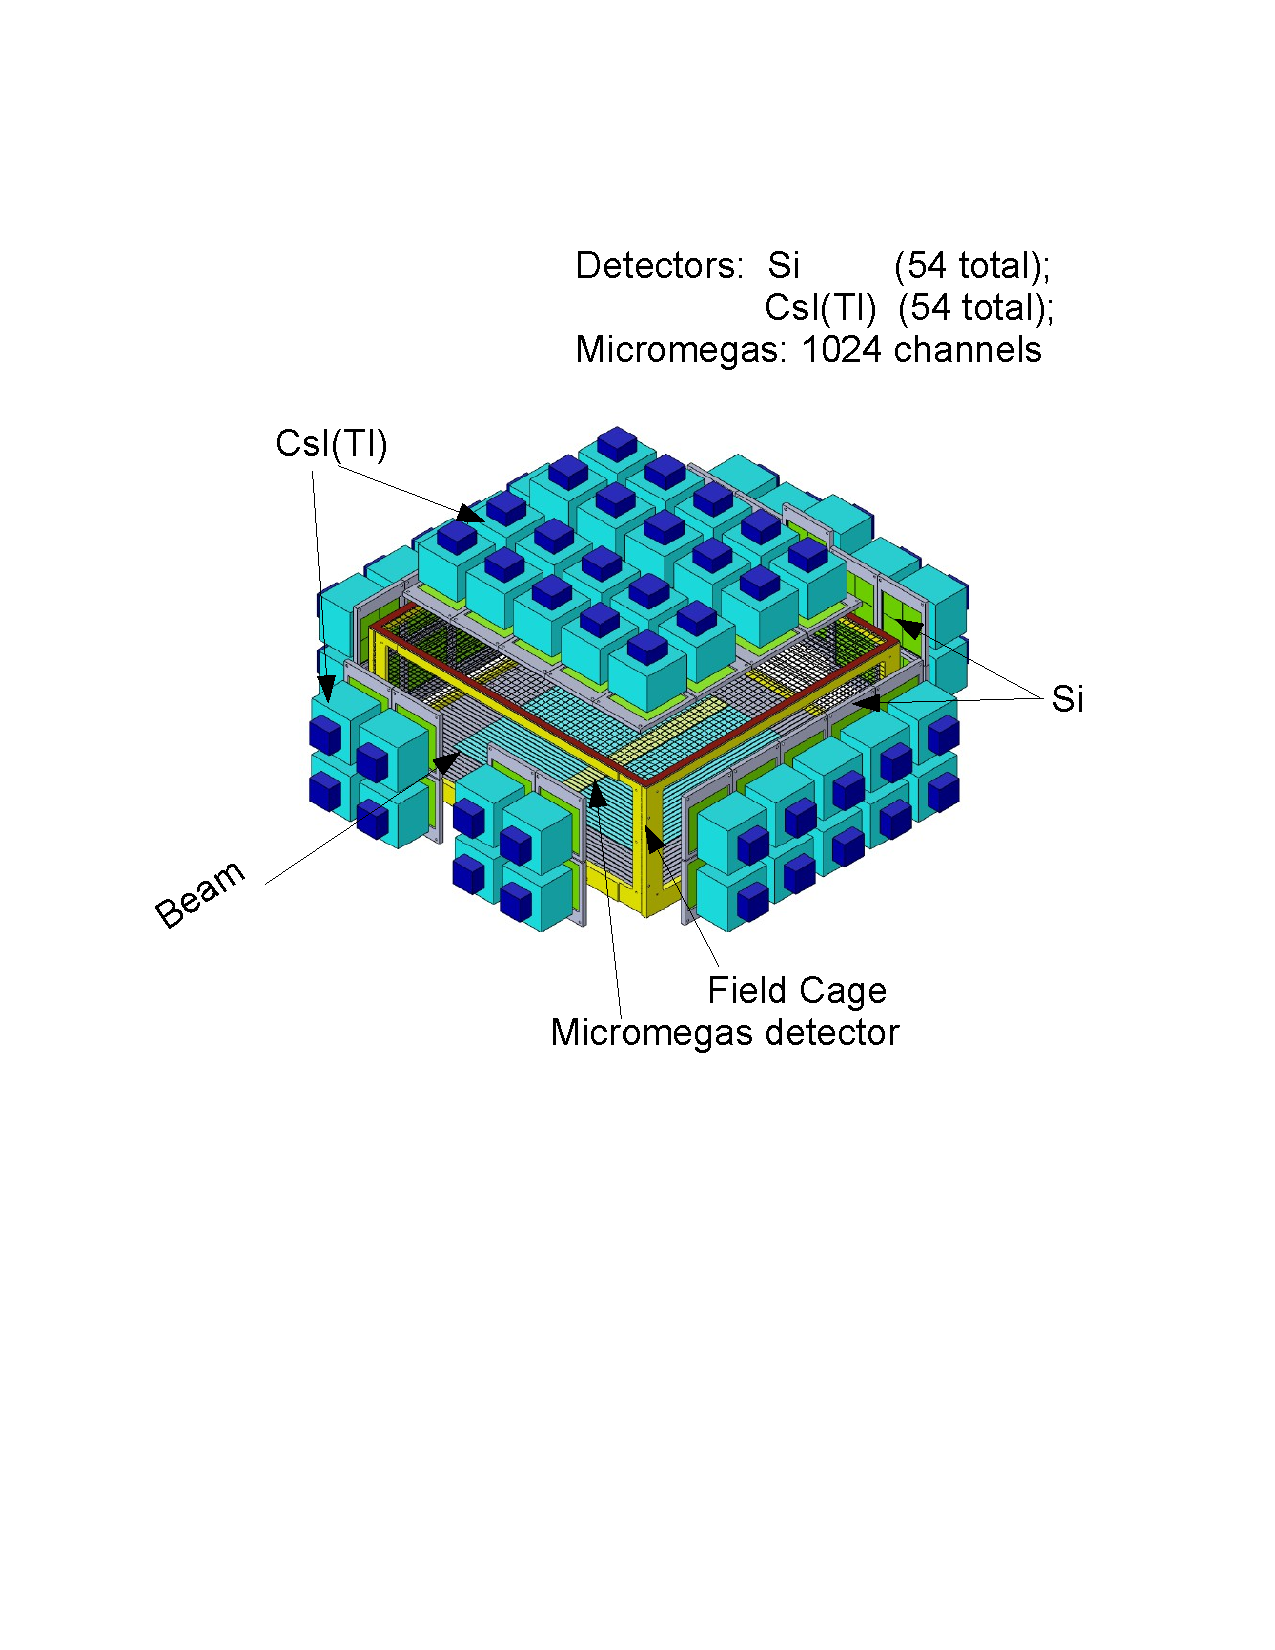
\includegraphics[width=1.0\columnwidth]{figs/TexAT_Assembly}
    \caption{Sketch of TexAT Assembly. Detailed description of the individual components is provided in the text.} 
   \label{fig:TexAT_Assembly}
\end{figure}

\subsubsection{Time Projection Chamber}
	
Two main components of the TexAT TPC are Micromegas detector and a Field Cage.
		
The key element  is a Micromegas (Micro-MEsh GAseous Structures) detector \cite{Micromegas_1, Micromegas_2}. It consists  of a highly segmented anode readout board with a stretched above it a woven metallic mesh. Such geometry creates a  parallel- plate gas- electron amplification volume, where the  primary electrons, generated by ionization in the active ``drift'' volume of the detector are amplified. It is basically an``ideal'' parallel- plate gas-electron proportional counter.  The electric field between the micro- mesh and the readout plane, which is on the order of few tens of kV/cm, is much greater than the field in the drift volume above the micromesh.

A Field Cage above the micromesh provides a uniform electric field in the active volume. Generally, this field is on the order of $50$ V/cm to $1$ kV/cm. A detailed description of the field cage is given in Sec. \ref{FieldCage}.

The custom  Micromegas detector for TexAT was designed in collaboration with IRFU (Sacle, France) and fabricated at CERN using "bulk"- technology: the readout board, a photo-resist layer (128 $\mu$m thick) and the cloth mesh  (Stainless- steel wires of 30 $\mu$m diameter interwoven at a pitch of 80 $\mu$m)  were encapsulated together and then etched, producing the pillars of 300 $\mu$m diameter and a pitch of 2 mm in one single process \cite{GIOMATARIS2006}. The amplification gap (avalanche area) of 128 $\mu$m between anode pads and embedded mesh allows for gas gains of up to the 10$^{4}$-10$^{5}$. It has been demonstrated that this gain is sufficient to observe proton tracks with characteristic specific energy loss on the order of keV per mm.

\subsubsection{Micromegas Detector Readout Board Configuration}
	
A rectangular (346 mm  x 316 mm) Micromegas PCB has an active area of 224 mm x 240 mm. To reduce the total number of channels  a unique segmentation/multiplexing scheme was conceived, consisting of rectangular pads in the beam region and overlapping strips and chains to the left and right of the central region. The total number of Micromegas readout channels is 1,024. The board  is divided into three areas as shown in Fig. ~\ref{fig:MMBoardLayout}: the zone to the left of a beam axis (L), the beam axis zone (C) and the zone to the right of the beam axis (R).

\begin{figure}[hbt!]
    \centering
     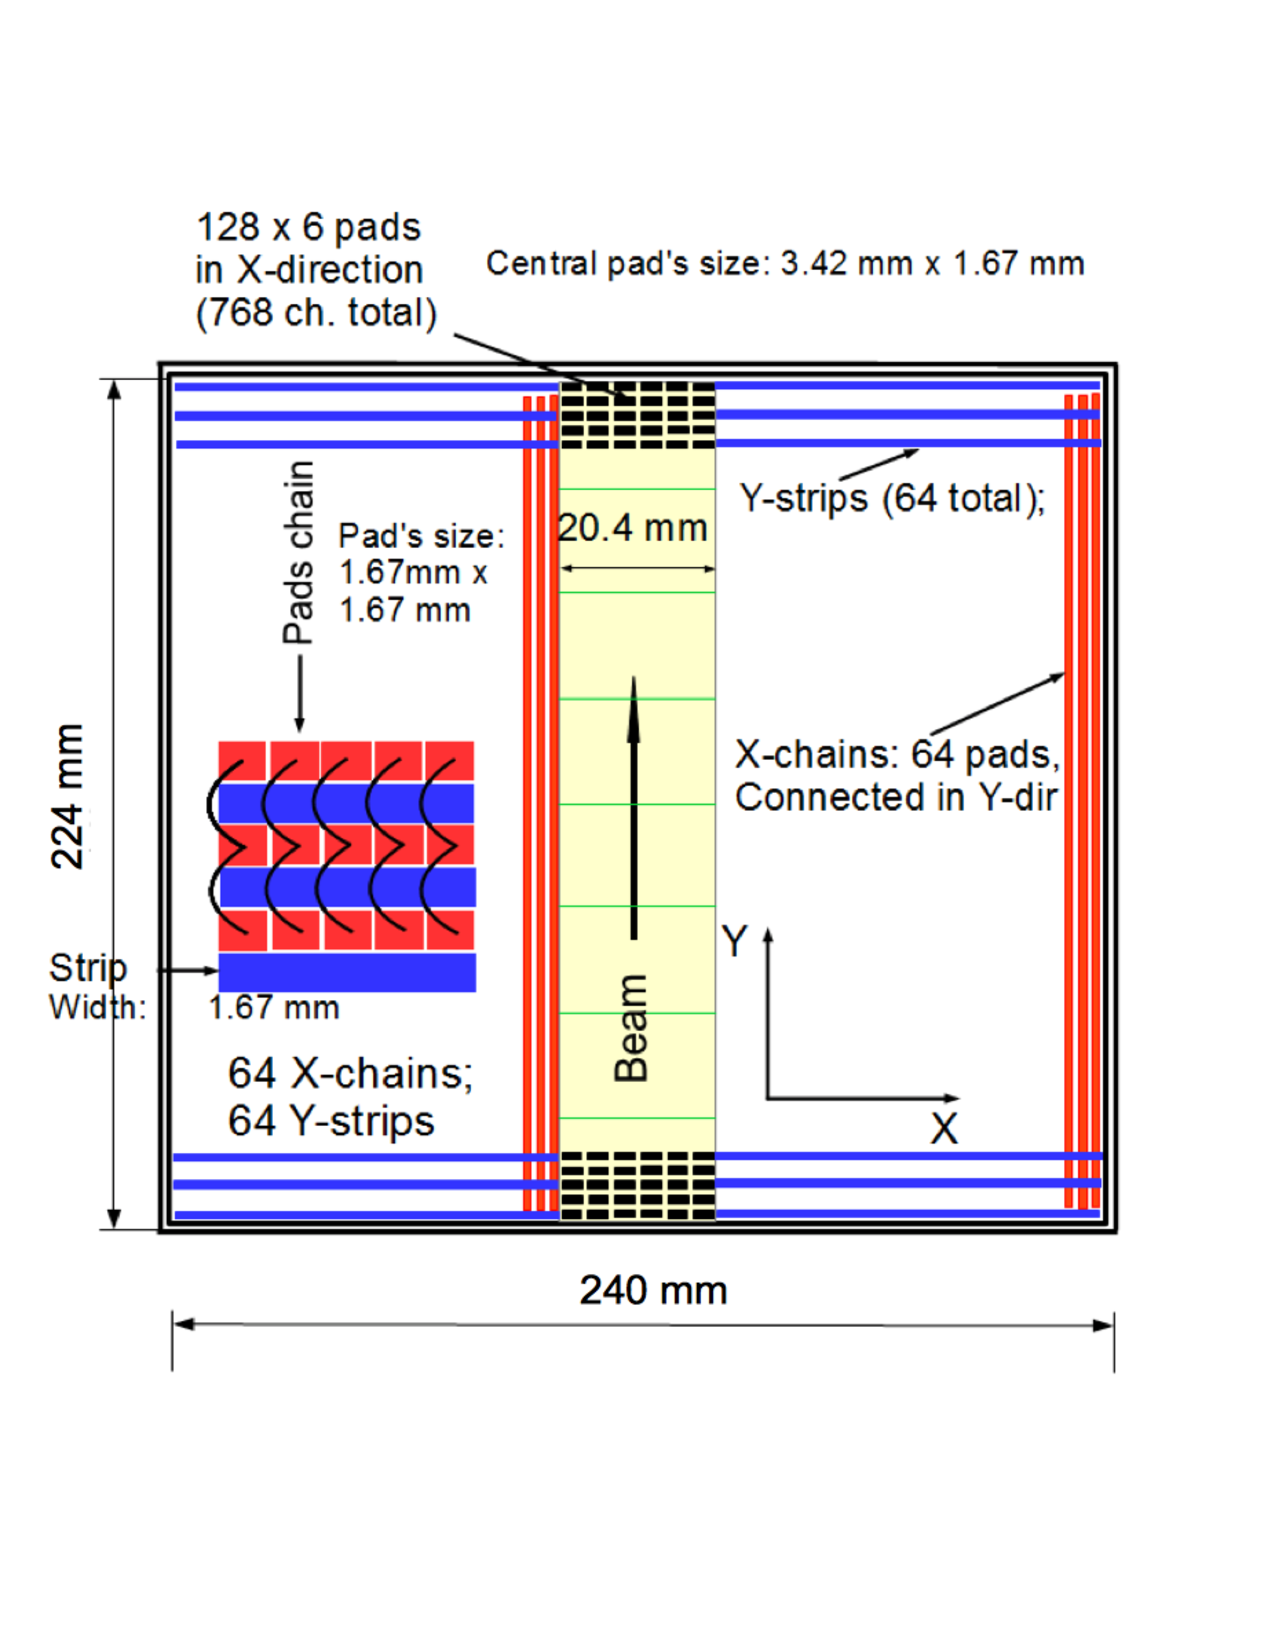
\includegraphics[width=1.0\columnwidth]{Figs/MMBoardLayout}
    %\caption{Micromegas PC board design}
%\end{figure}
%\begin{figure}[ht]
 %   \centering
    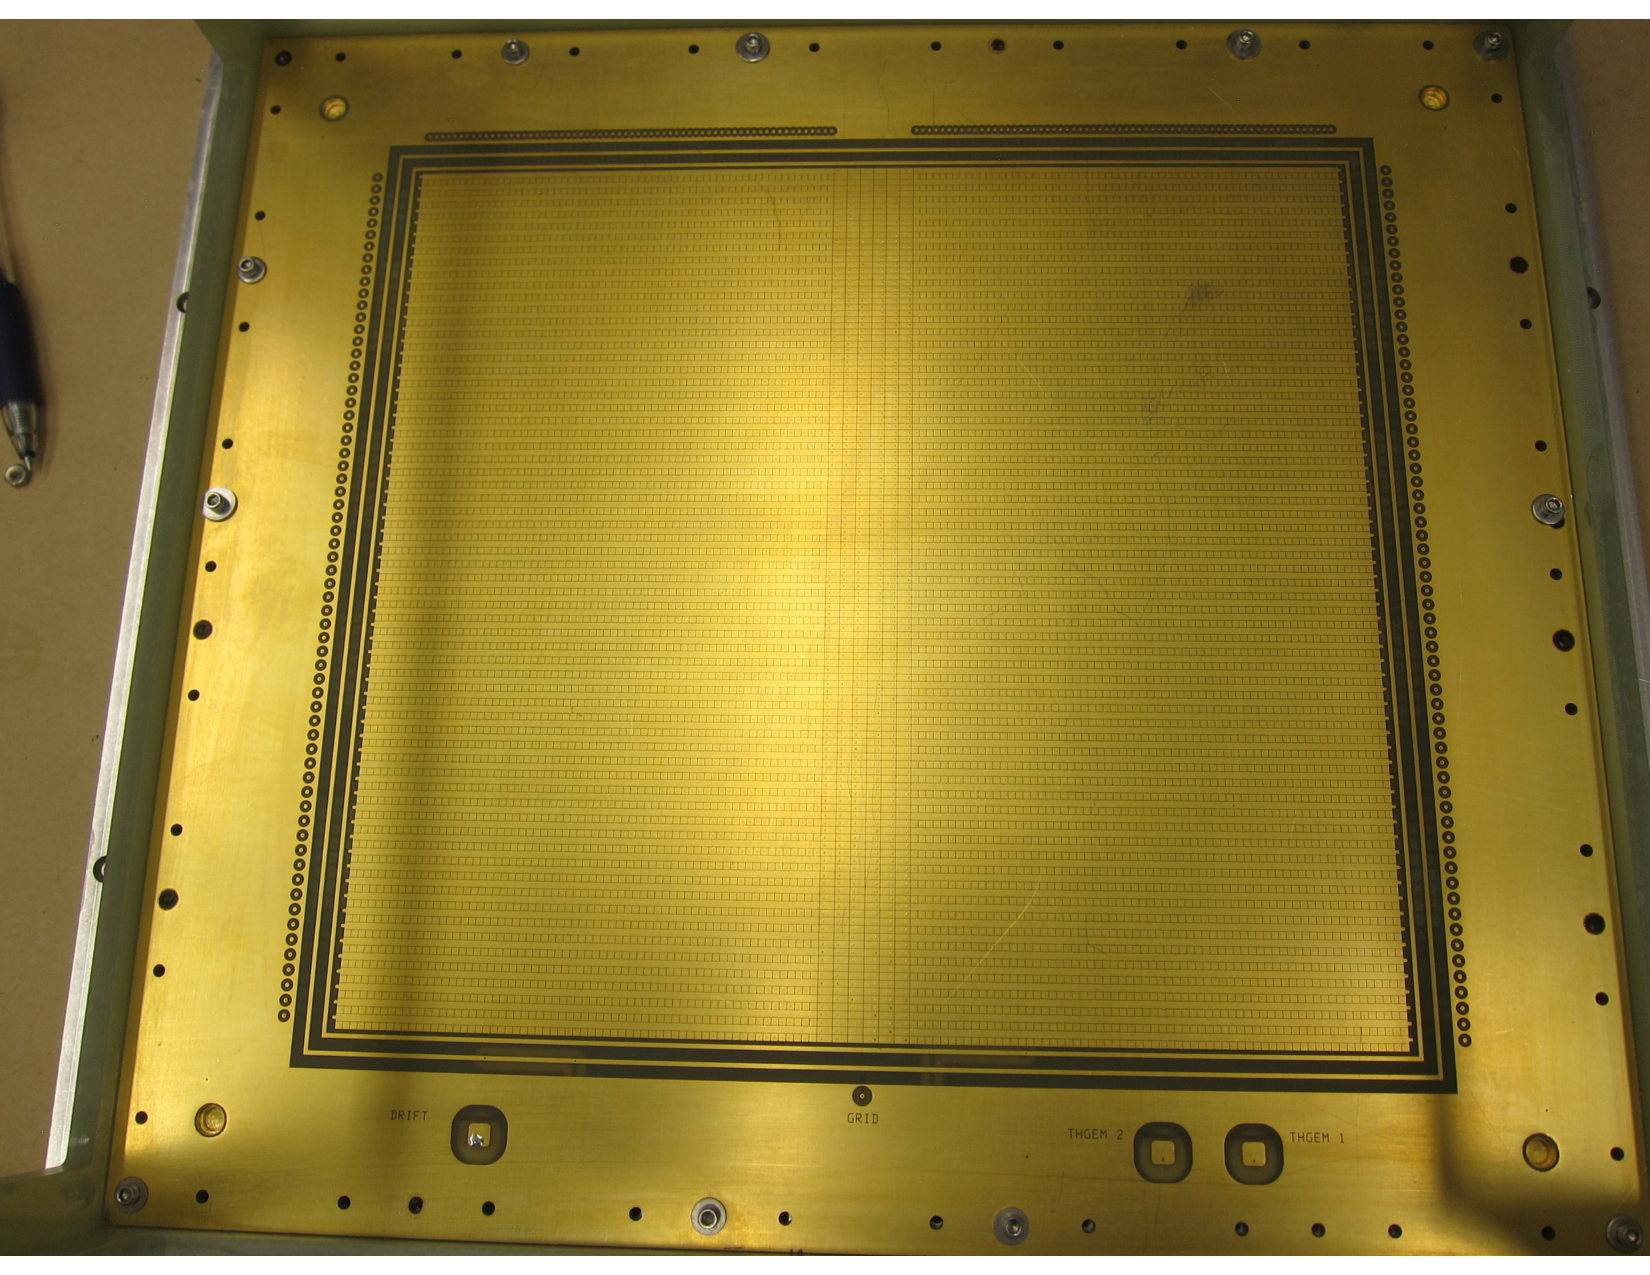
\includegraphics[width=1.0\columnwidth]{Figs/MMBoard}
    \caption{Top panel: The design of an active area of Micromegas PCB (to be modified - make "side- pads of central area in different color. {Picture of the Micromegas readout plane showing the detection pads. Shows the rows of the central pads consisting of six columns. The strips in the side planes are the solid readout pads that are perpendicular to the beam axis while the chains are the square readout pads in the side regions that go along the beam axis.} )
        Bottom panel: Foto of readout board. }
        \label{fig:MMBoardLayout}
\end{figure}

Central zone (shown in yellow in Fig. ~\ref{fig:MMBoardLayout}, top panel) along the beam axis is 20.4 mm wide and has high segmentation: 128 x 6=768 individual pads (the pad size is 1.67mm x 3.42 mm). The pads are arranged so that there are 128 pads in the direction of the beam (along 224 mm side) and 6 pads in the direction perpendicular to the beam.

Both left (L) and right (R) zones are identical and have dimension of 224 mm x 101.5 mm. Each consists of 64 strips, perpendicular to the beam axis. The strip is 1.67mm  x 101.5mm. There is 1.75 mm space between strips to allow for an individual pad to be placed between the strips. Distance between the centers of the strips is 3.5 mm. There are 64 individual 1.67 mm  x 1.67 mm pads between each two strips. The pads located at the same distance from the beam axis are connected into chains, so that there are 64 ``chains'' of 64 interconnected pads arranged in the direction parallel to the beams axis in each of the side zones. Although the strips and chains individually cannot provide an accurate location for tracking because each strip and chain run along either the beam axis or perpendicular to the beam axis, they can be matched together to make a 2D point (see Section \ref{CSmatching}). A picture of the actual TexAT Micromegas readout board without the mesh (the blank) is shown in the bottom panel of Fig.~\ref{fig:MMBoardLayout}.
	
The signal readout of Micromegas board is carried out trough the 80-pin (only 64 channels are active) high density (0.8 mm pitch) Edge
 Rate\textsuperscript{\textregistered} Rugged High-Speed  {SAMTEC} connectors. An optimized signal readout channel map has been designed. According to this map PC board has been segmented into different geometric zones of 64 channels:
\begin{itemize}
  \item the central ("Beam") area (4 most central pads in each of 256 rows, 768 pads total) is divided to eight zones (shown by green lines in the top panel of Fig.~\ref{fig:MMBoardLayout}.
  \item the left- and right- side pads of central area form two columns of 2 $\times$64 pads each (shown by cyan in the top panel of Fig.~\ref{fig:MMBoardLayout}).
  \item zone (L) and (R) are parted in the following way:  the group of 32 upstream strips and 32 far from the beam area chains combine into single readout zone; the 32 downstream (top at  Fig.~\ref{fig:MMBoardLayout} strips and 32 close to the center chains make another one.
  \end{itemize}

Following the form- factor of the readout electronics, described in Section \ref{GET}, the zone's readout is organized in specified way: 2$\times$256 channels from the most central  area;  256 channels from the Left Zone (2 x 64 strips and chains) and left side- columns of the central zone (2 x 64 pads), and 256 channels from the Right Zone (2 x 64 chips and chains) and right side- columns of the central zone (2 x 64 pads).

Such segmentation facilitates the signal routing and allows to individually bias pads in the separate zones, giving a possibility to create an avalanche areas with different gas gains within the single Micromegas detector. It will be shown below (see Section \ref{lowANDhigh}) how useful this feature is.

\subsection{Field cage \label{FieldCage}}

Transparent for the beam ions and reaction products field cage maintains the uniform electric field inside a TPC volume with sufficient  strength to provide a steady drift of electrons.  The basic geometry of the cage surrounding the TPC is constrained by given Micromegas readout board design and the solid state detector's wall design: 316 mm (L) x 346 mm (W) x 135mm (H).  A 50 $\mu$m (diameter) gold plated tungsten wire has been chosen as the main element for the cage. The conversion drift volume is located between a transparent cathode, which is normally set to the high ``negative'' potential ($\>$ -1000  $\div$   - 3000 V) and a grounded mesh, transparent for electrons. The electrons released in collision of charged products with a the target gas drift toward positively biased Micromegas pads, through the mesh. The homogeneous electric field is supported by the set of guide wires, stretched along the walls perimeter, stepped down from the negative potential  of the cathode to the anode continuously by the voltage division, using a series of 25 MOhm resistors to create a uniform electric field. The resistors were hand-picked within tolerance of 0.5 $\%$.		 	 
	 
A 3D- model of the TexAT field cage (shown in Figure~\ref{fig:FieldCageSim}) has been created using a finite element mesh generator GMSH\cite{GMSH}.  To estimate a level of electric field uniformity and optimize wires spacing to create the best condition for electron drift inside the TPC,  the detailed simulations with computer codes GARFIELD \cite{GARFIELD} interfaced with Elmer \cite{Elmer} have been performed.
		
			
\begin{figure}[hbt!]
    \centering
    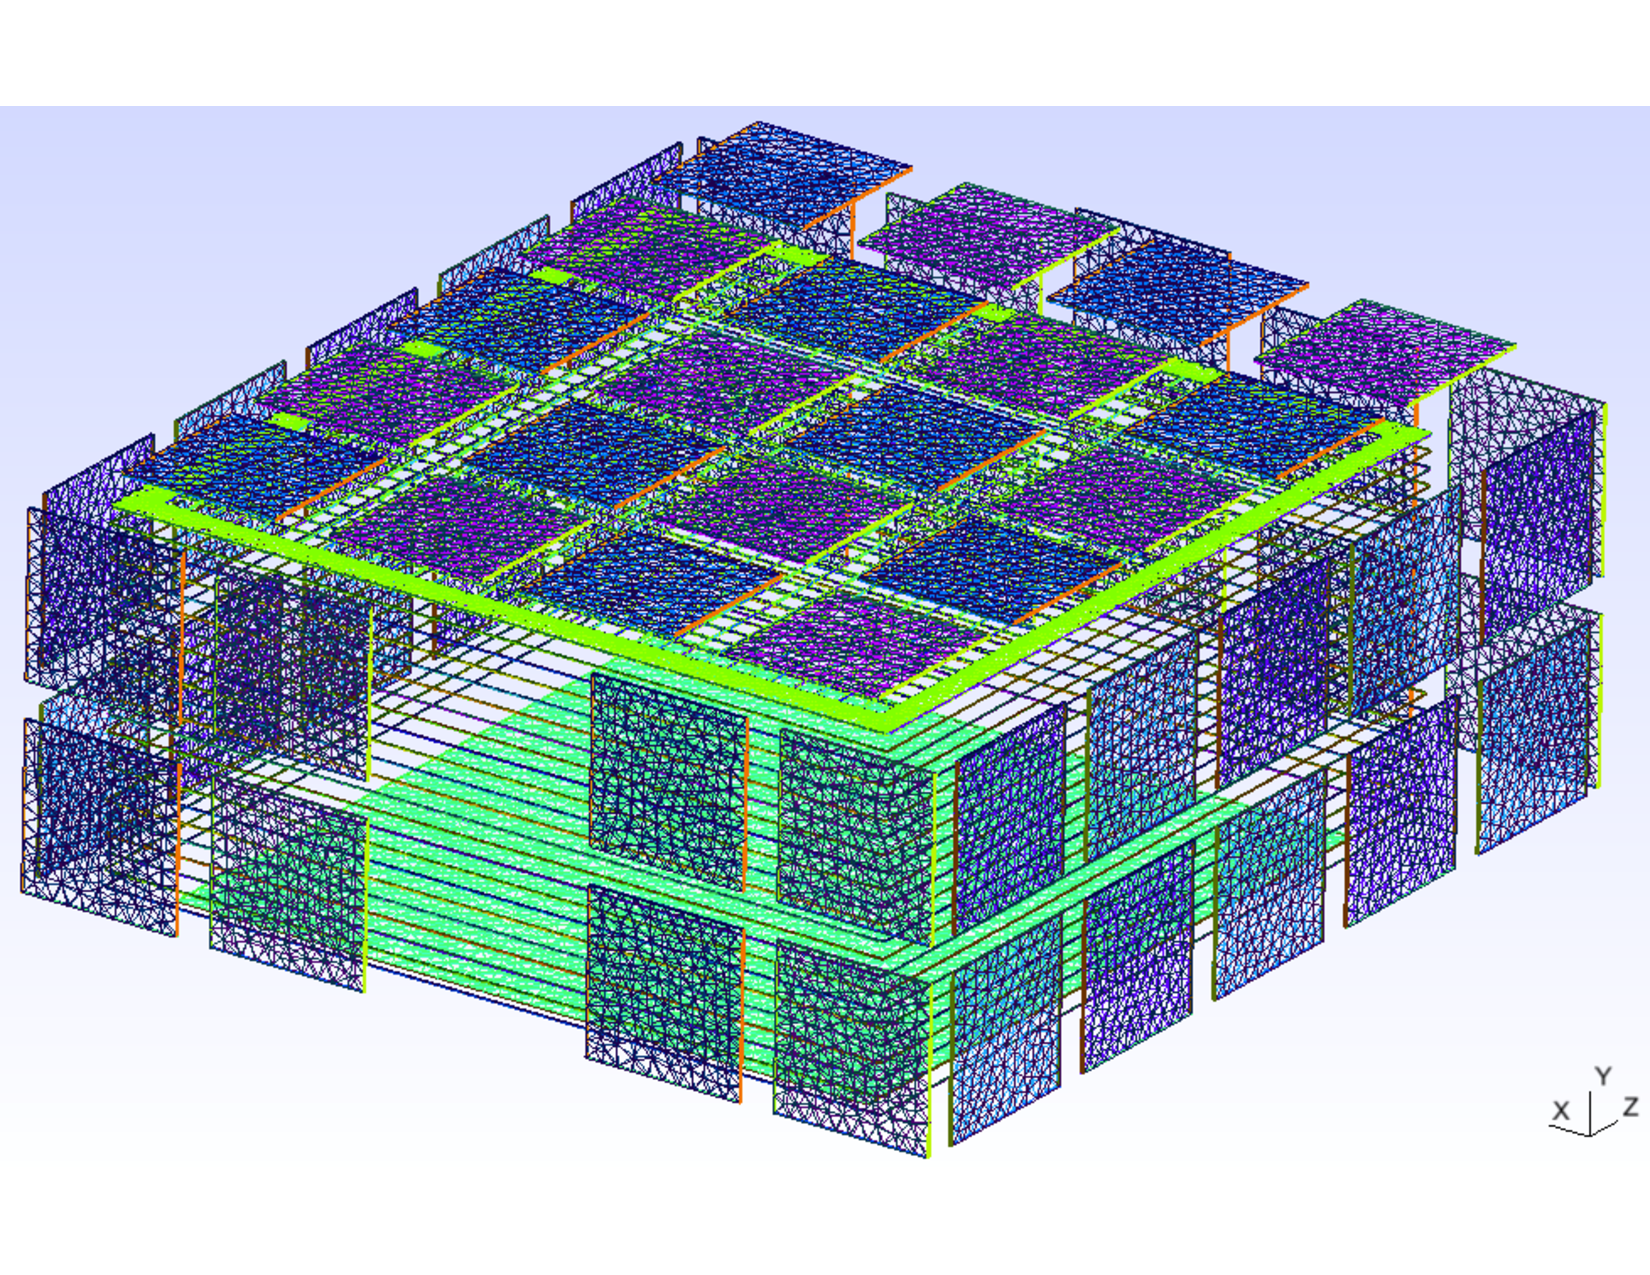
\includegraphics[width=1.0\columnwidth]{Figs/FieldCageSim}	
    \caption{Simulated model of field cage for TexAT.}
     \label{fig:FieldCageSim} 
\end{figure}
		
The  Elmer Solver's Finite Element Analysis provides a  map of the electric field at every point in the TPC. A simulated 3D- plot of electrostatic field map inside TexAT TPC (the front of surrounding Si- detectors is grounded) is  shown at  Figure ~\ref{fig:Field3D}.  One can see that computed field appears to be pretty steady inside an active TPC volume while some deviations are  manifested in the areas near  boundaries of the cage and close to Micromegas mesh.  The aberrations of field uniformity  are apparently  induced by the leak of electric field through the transparent cage and mesh. 

The simulation of  "realistic" configuration (front side of Si- detectors is under full depletion potential of -200 V is shown in Figs. ~\ref{fig:FieldXZ} and \ref{fig:FieldXY}. A particular geometry of surrounding detectors enhances non-uniformity effect, especially at the "downstream"-side  wall, that has a non-symmetric  geometry (see Section \ref{Si} below).

The "edge"-  effects distort the electric force lines near the  walls and create a dependence on the position of the track. These deviations can be reduced to some extend by increasing the guide wires density, but a compromise between a transparency factor, acceptable level of uniformity, and a practical fabrication has to be established. It has been determined, that the wire spacing of 5 mm provides a sufficient level of electric field uniformity inside the active volume of TPC.  The 5 mm spacing allows for wire to be mounted on extension springs to avoid wire sagging, the technique developed for ANASEN detector \cite{ANASEN}.
		 		 
\begin{figure}[hbt!]
    \centering
 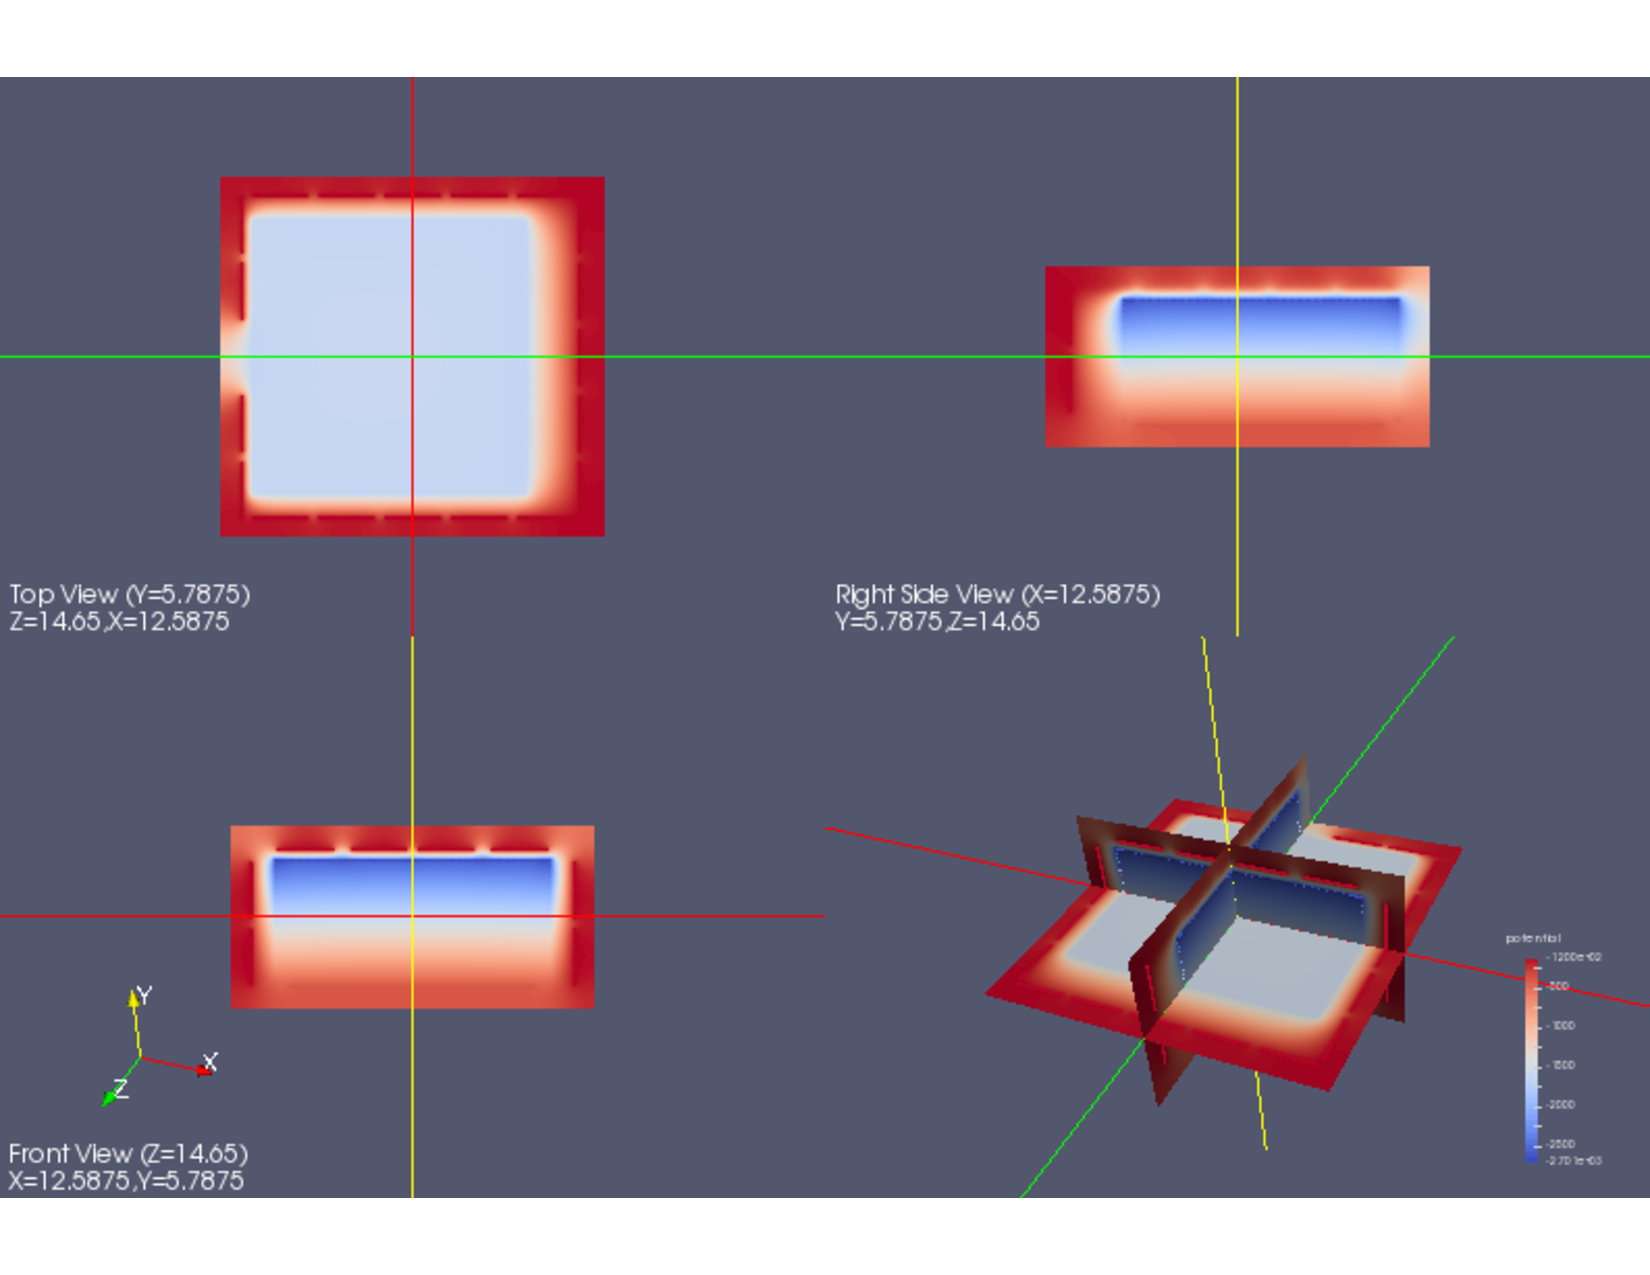
\includegraphics[width=1.0\columnwidth]{Figs/Field3D}	
    \caption{Electric field simulation}
     \label{fig:Field3D} 
\end{figure}
		
\begin{figure}[hbt!]
    \centering
 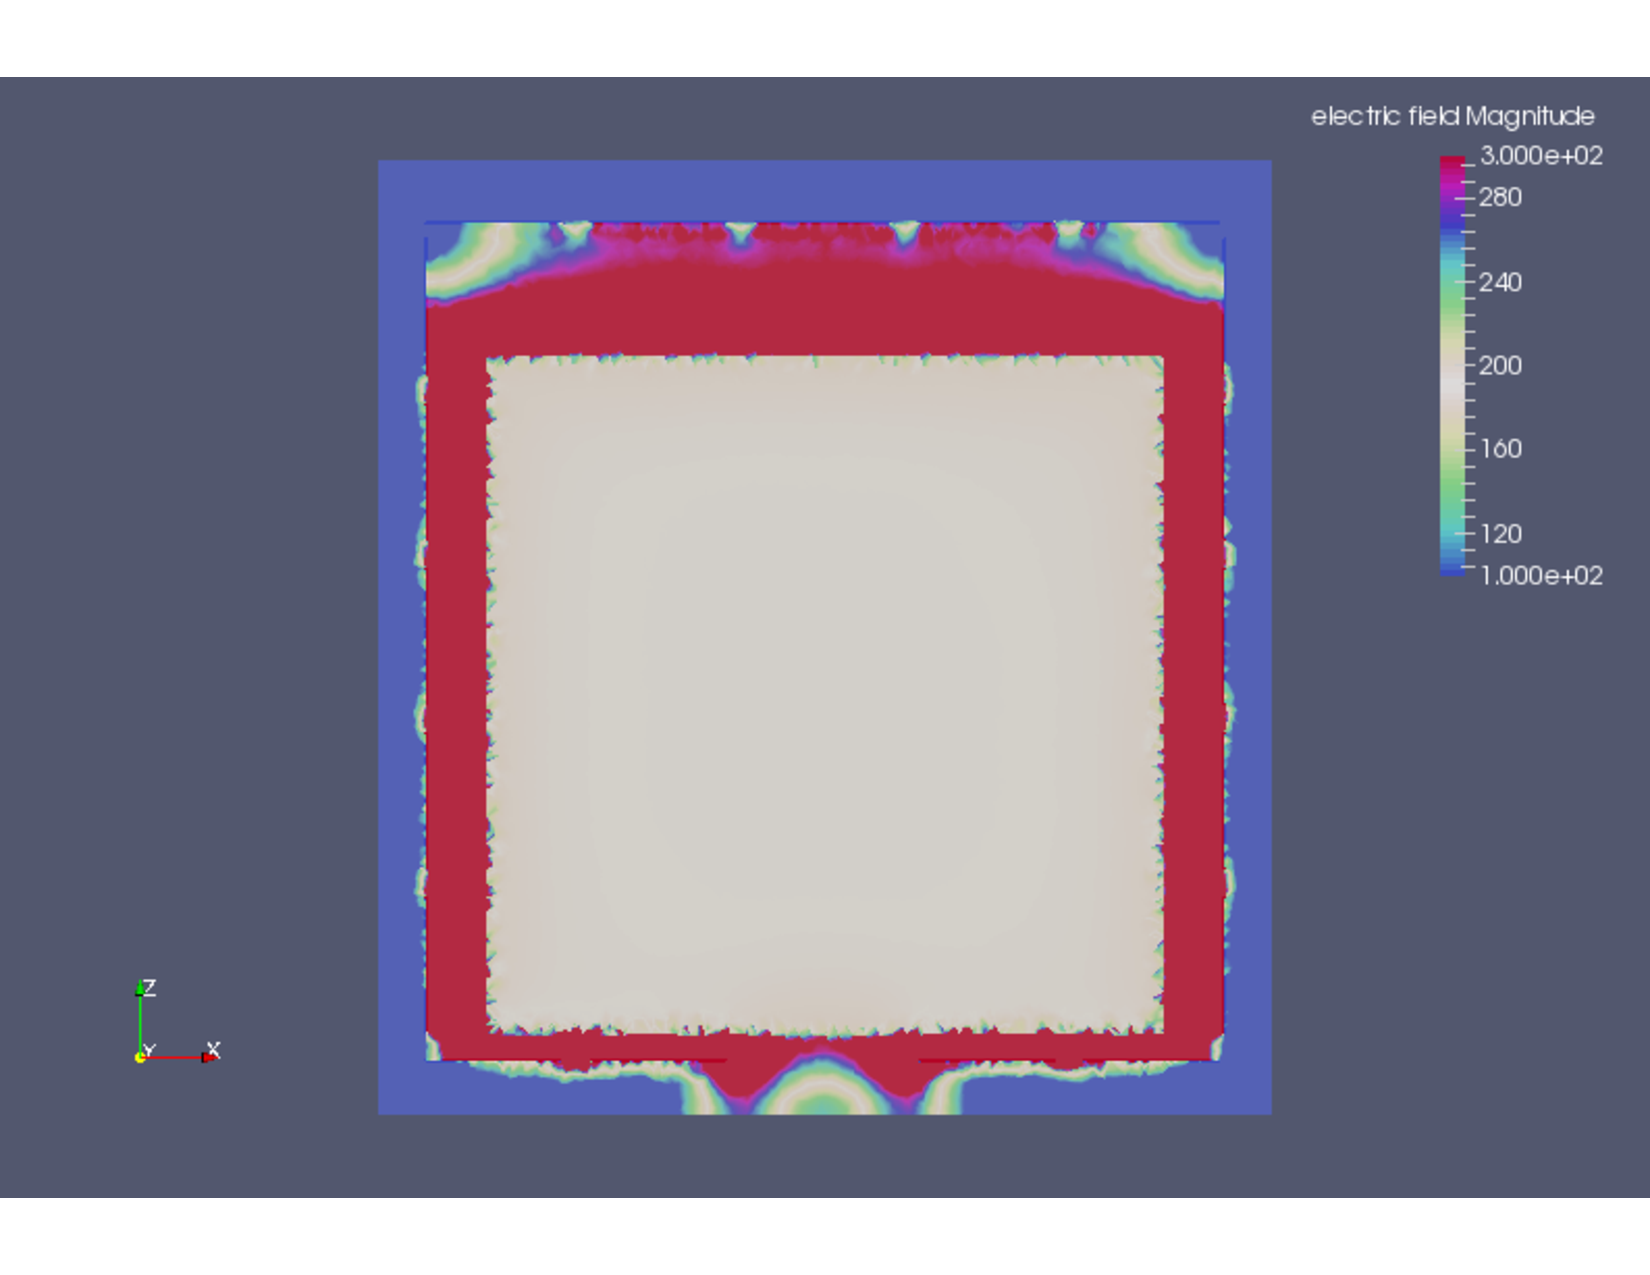
\includegraphics[width=1.0\columnwidth]{Figs/FieldXZ}	
    \caption{Electric field simulation: Top  (XZ plane)  view}
     \label{fig:FieldXZ} 
\end{figure}
		
		
\begin{figure}[hbt!]
    \centering
 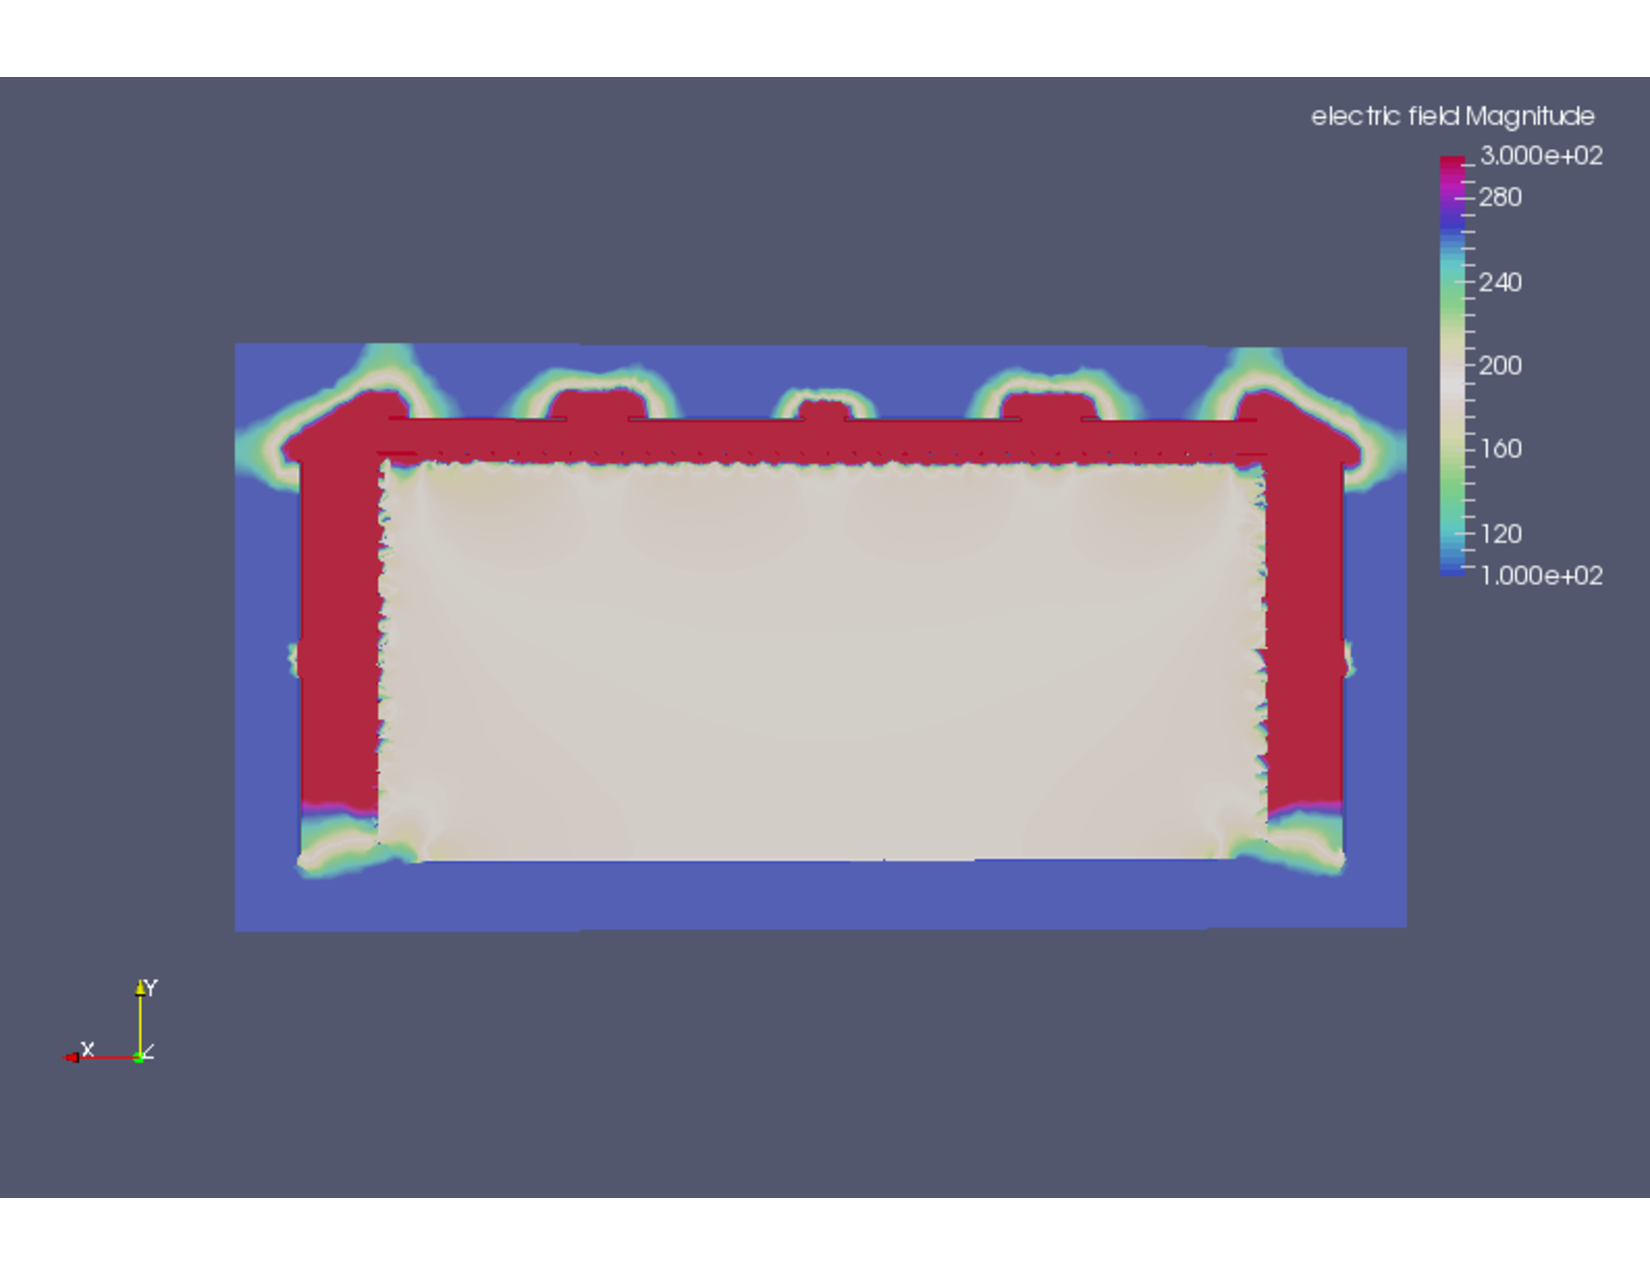
\includegraphics[width=1.0\columnwidth]{Figs/FieldXY}	
    \caption{Electric field simulation: Side (XY plane) view}
     \label{fig:FieldXY} 
\end{figure}
	
The leak of positive potential on the pads through the transparent grounded mesh leads to the perceptible distortion of electric field (at the level of 10 $\div$ 15$\%$) near the mesh, which separates the ``drift'' volume from the ``avalanche'' region. This effect is unavoidable because of particular geometry, but further computation of electron transport in different gases (Methane, Butane, Ar/CO2, He/CO2 mixtures) using MAGBOLTZ \cite{MAGBOLTZ} have defined the optimal conditions for constant electron drift velocity even in the presence of electric field aberrations.  One example of such simulations is shown in Fig. ~\ref{fig:FieldVsP} for Methane gas at different pressure.  The "Navy Blue"- colored (shown online) area at the plot represents the optimal conditions for electron drift.
 
\begin{figure}[hbt!]
    \centering
   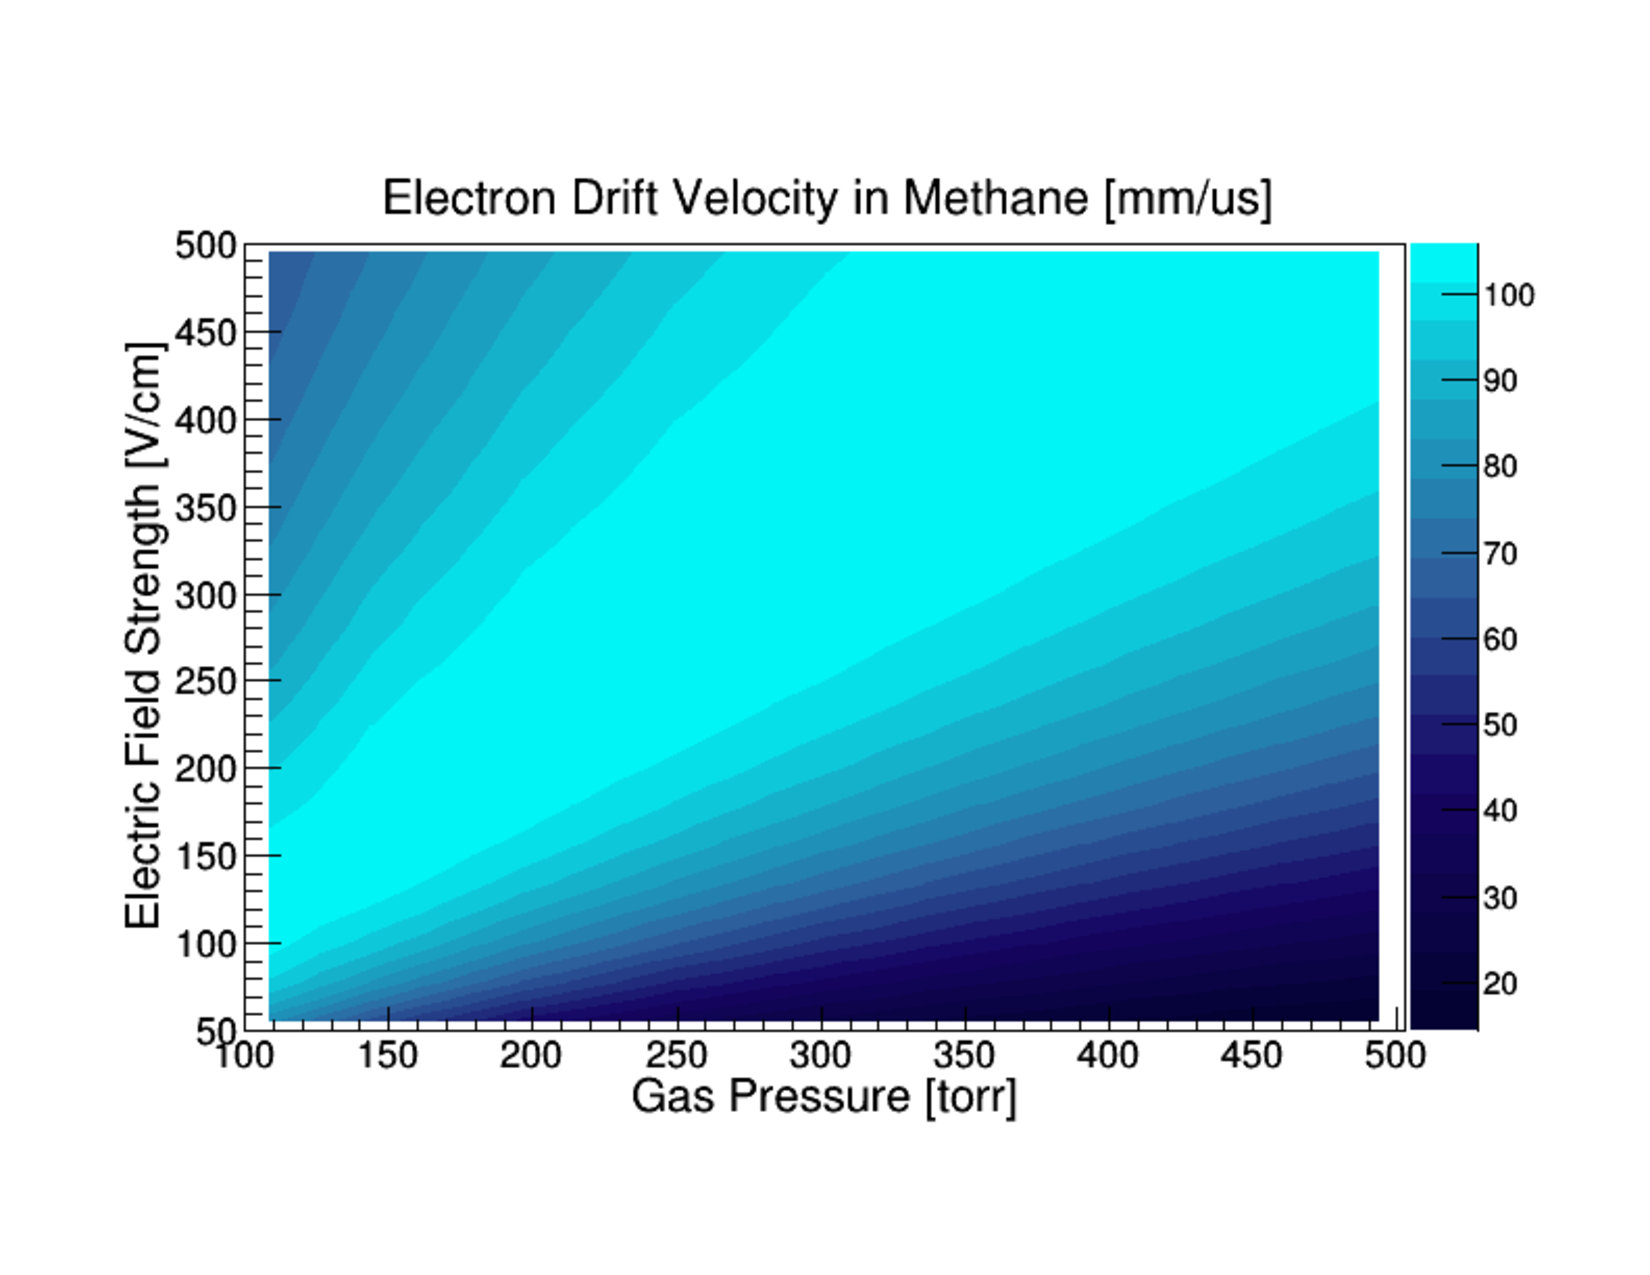
\includegraphics[width=1.0\columnwidth]{Figs/FieldVsP}	
    \caption{Electron drift time for different gas pressure and field strength}
     \label{fig:FieldVsP} 
\end{figure}
		
Another factor, that may deform an electric field  is an "axial" geometry of the guide wires, instead of a classic "plane" guides. A  horizontal electric field between the field cage and the walls leaks in the drift region, deforming the electron drift trajectory. To investigate the effect of this factor, a TPC prototype with a  "single wire" field cage has been tested with different gases. Analysis of timing characteristics of $\alpha$-particle tracks from the source (drift time versus position at Micromegas) reveals the non- uniformity effects at the entry of Micromegas detector.  The noticeable deviations from linearity (circled in Red) are shown in Fig. ~\ref{fig:tracks} inside. This effect is especially notable in the case of slow electron drift velocity (in gasses such as Helium+ 2\% CO$_2$ mixture). 

To improve linearity near the edges the second set of wires was introduced at a horizontal distance of 5 mm from the first set, as shown in Fig.~\ref{fig:DoubleGrid}. This second layer establishes the flat iso-potential ``surfaces''. It was shown that more in-plane wires would not affect the iso-potential surfaces nearly as much as just adding that second point/wire.
The two wire cage with 5 mm vertical spacing and 5 mm horizontal distance between the two wires satisfied the condition of minimum non-uniformity of the electric field, 98\% transparency and practical fabrication considerations.

\begin{figure}[hbt!]
    \centering
    \includegraphics[height=1.7\columnwidth]{Figs/distort}
    \caption{Single Events old  FieldCage.   X-axis:  Position in Micromegas ("0" represents the entrance of Micromegas), Y-axis:  Drift time. The collimated $\alpha$- source is located upstream. 
    The non-linearity of the tracks close to the entrance area can be seen.    This picture will be replaced!!!!!}
      \label{fig:distort} 
\end{figure}

\begin{figure}[hbt!]
  \centering
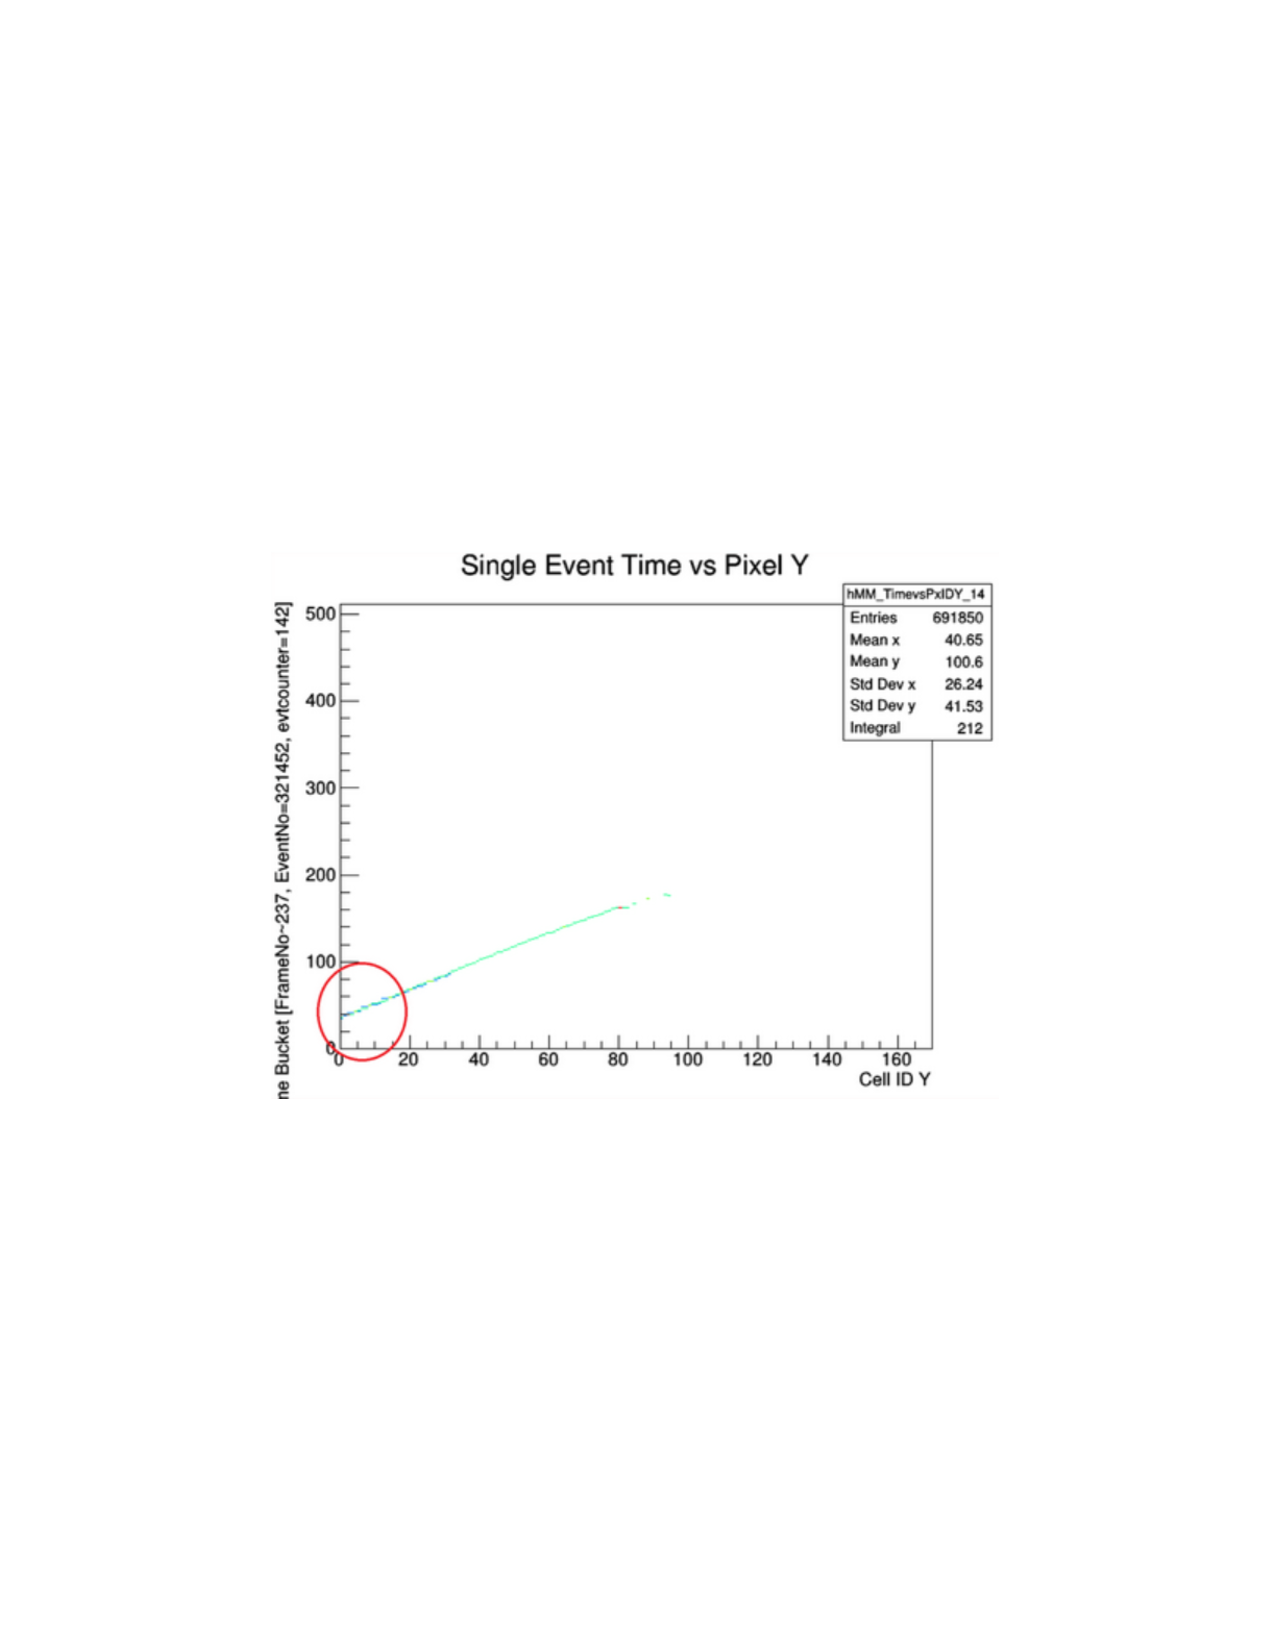
\includegraphics[width=1.0\columnwidth]{Figs/tracks}
  \caption{""Timing"- track  of $\alpha$- particles in He+2$\%$CO$_2$ mixture (top panel) and P5 (bottom panel) gas. X-axis:  Micromegas pad number  ("0" represents the entrance of Micromegas), Y-axis:  Drift time. The collimated $\alpha$- source is located upstream, making tracks almost parallel to the Micromegas plane. The non-linearity of the tracks close to the entrance area can be seen.   This picture will be replaced!!!!! }
    \label{fig:tracks} 
	\end{figure}

\begin{figure}[hbt!]
    \centering
    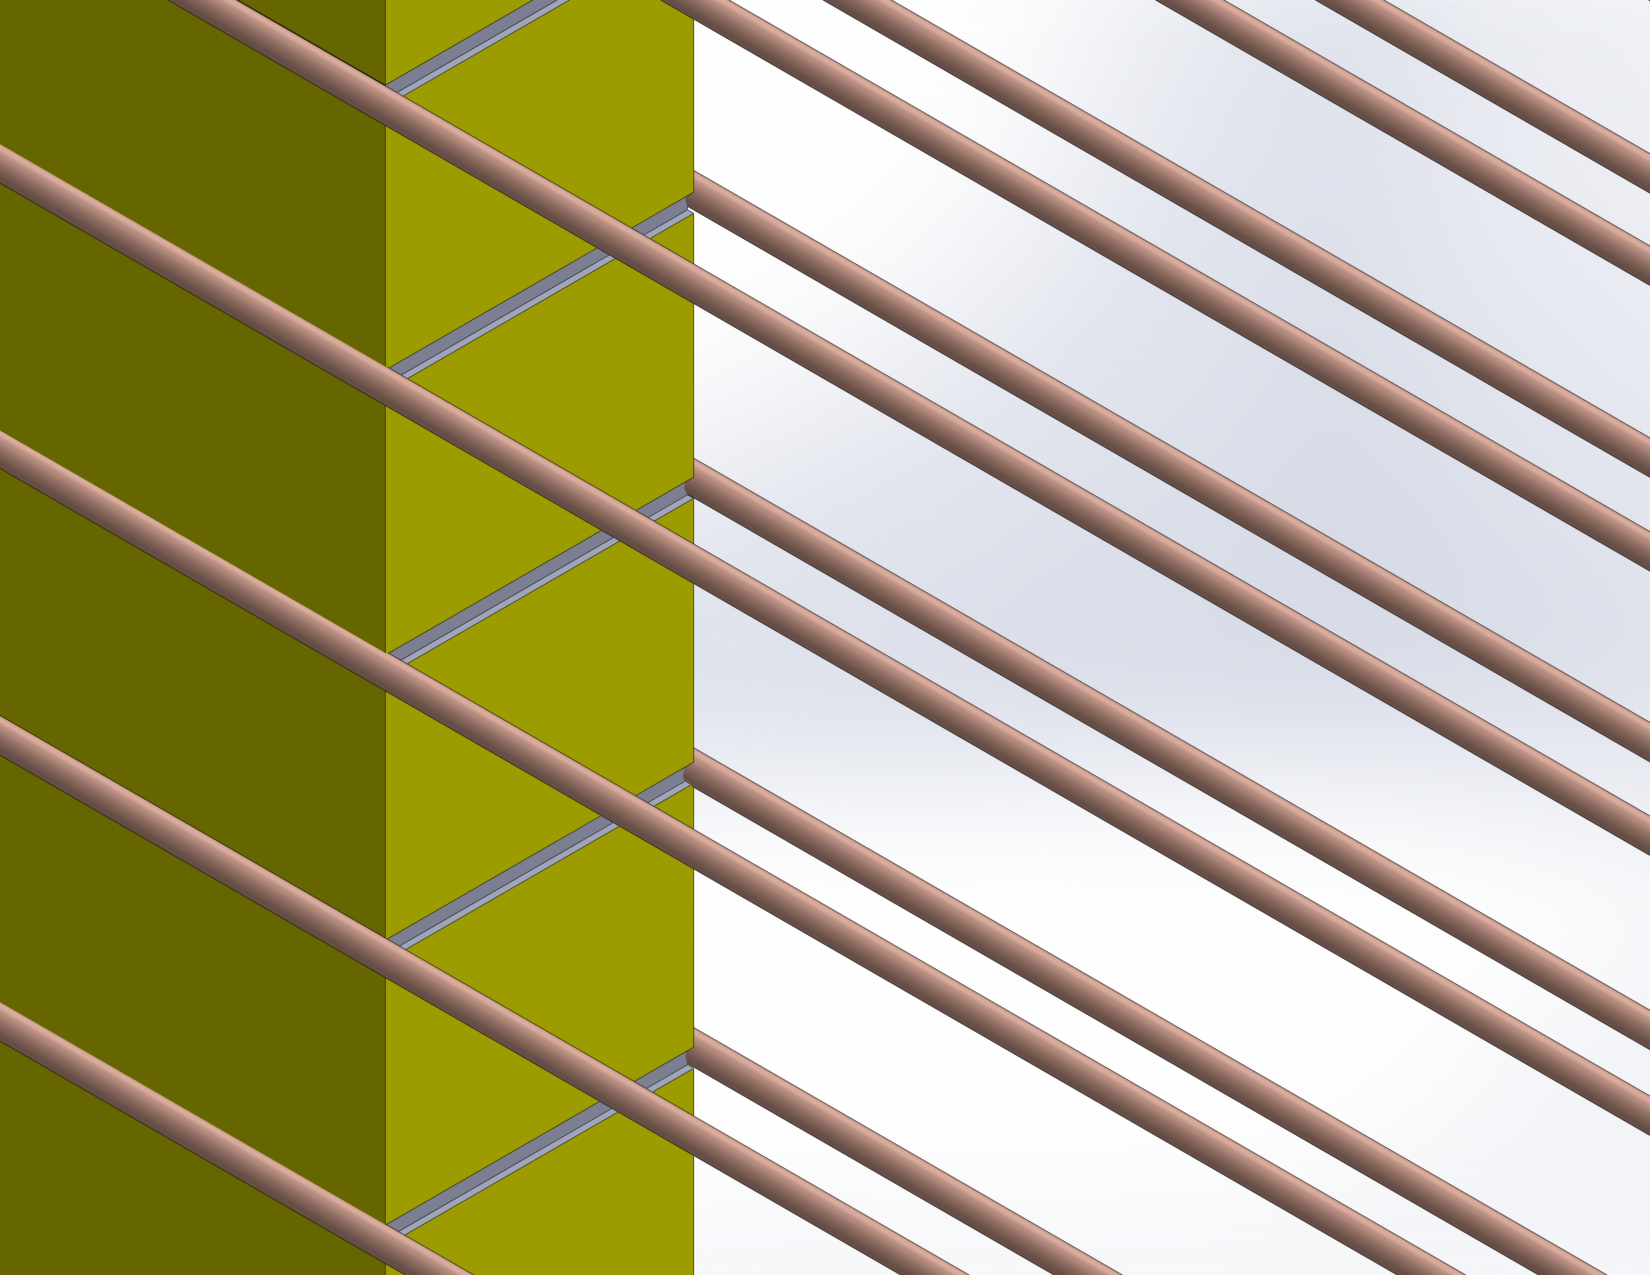
\includegraphics[width=7cm]{Figs/DoubleGrid}
    \caption{Double Layer Grid}
  \label{fig:DoubleGrid}
\end{figure}


\subsection{Solid state detector array \label{Si}}

Arrays of solid state detectors (Si and CsI) are used in TexAT to measure a total energy of particles escaped the active target volume and to provide an additional PID. Due to 3D tracking in the TPC, high segmentation for the Si- wall is not necessary. Double side silicon detectors with an active area of 50$\times$50 mm$^2$ were chosen to build a Si- detector walls, surrounding the TPC. The principal requirements were high energy resolution, reliability and price to quality measure. 

A three different types of Si- detectors were used:
\begin{itemize}
  \item MSQ25-1000 from Micron Semiconductor (\cite{Micron}). The geometry is: four quadrant sectors (25$\times$25 mm$^2$) at junction side and single quadrant (50$\times$50 mm$^2$) at ohmic  side. The typical energy resolution for $\alpha$ particles from the $^{241}$Am source is 50 - 70 keV, and the total  leakage current at full depletion is less then 1 $\mu$A (degraded  to 3 $\mu$A after several in-beam experiments);  
  \item W1-500 detector from Micron Semiconductor (\cite{Micron}). This detector is often used downstream at the beam axis. It has 16  vertical junction strips at the front  and 16 horizontal  ohmic strips at the back. The width of the strips is 3 mm. Such geometry provides a position sensitivity of 3 mm$^2$ allowing  a service diagnostic during the secondary beam development and  additional position sensitivity at small scattering angles for some experiments at low energy when beam stops in the gas target.
\item A test set of 12 total silicon four-segment charged particle detectors  KDP-1K  have been developed at the JSC ``Institute in Physical-Technical Problems'', Dubna, Russia  (\cite{SiDetDubna}) for TexAT.  The detectors were made of n-type Si (660 $\mu$m thick) using the ion implantation technology with thermal surface passivation. The input aperture of the detector is 54.1$\times$54.1 mm. The active area of each segment is 25.0$\times$25.0 mm$^2$ with a 50 micron gap between the segments. A system of common guard rings was used in the design of the detecting structures. The thickness of the detectors of the delivered batch was 625 micron. Detectors were tested both with alpha- source and in-beam. Typical leakage currents of the segment at a full depletion bias voltage of 130 V were found to be less then 20 - 30 nA. The spectrometric characteristics of each quadrant of the detectors were measured with alpha-  source at the over-depletion bias voltage of 150 V. Typical values of the energy resolution were at the level of 30 - 40 keV FWHM under irradiation from the pn junction side.  These detectors were in active use for 5 in-beam experiments and only one of 12 has lost a resolution below acceptable level (75 keV).  The properties of  KDP-1K detectors are in complience with technical requirements and it has been decided  to make them a basic component for TexAT.
\end{itemize}
  
The supporting frames are slightly different but in principle MSQ25-1000 and KDP-1K  are interchangeable  with some small adjustment. 

The outer layer of TexAT was composed from the thick CsI(Tl) scintillator detectors located at the back of all of the Si detectors. They can be used for detecting of both charged particles and gamma rays. Cuboid- shaped 40 mm thick CsI(Tl) crystals have been selected to ensure that the full energy is measured for particles that can penetrate through the silicon detector.The geometry of crystals was chosen to match Si detectors face: 50$\times$50 mm$^2$. Each crystal is wrapped in 2$\mu$m thick aluminized mylar, and has built-on preamp which are read out by single Hamamatsu 20$\times$20 cm$^2$ S3204 PIN diode. The role of CsI(Tl) array in the TexAT chamber is primarily to identify and measure residual energy of particles that punch-through the Si detectors. Using an $^{241}$Am alpha- source, we have determined the energy resolution for the CsI(Tl) detectors to be about 5\%.

Solid state telescopes are arranged in 4 different configuration matching TPC geometry (shown in Fig. ~\ref{fig:WallsAll}). All side's arrays  are mounted at independent doors providing an easy excess to the scattering chamber and handy replacement of components. The bottom array is placed onto the main body of the TexAT scattering chamber.


\begin{figure}[hbt!]
    \centering
    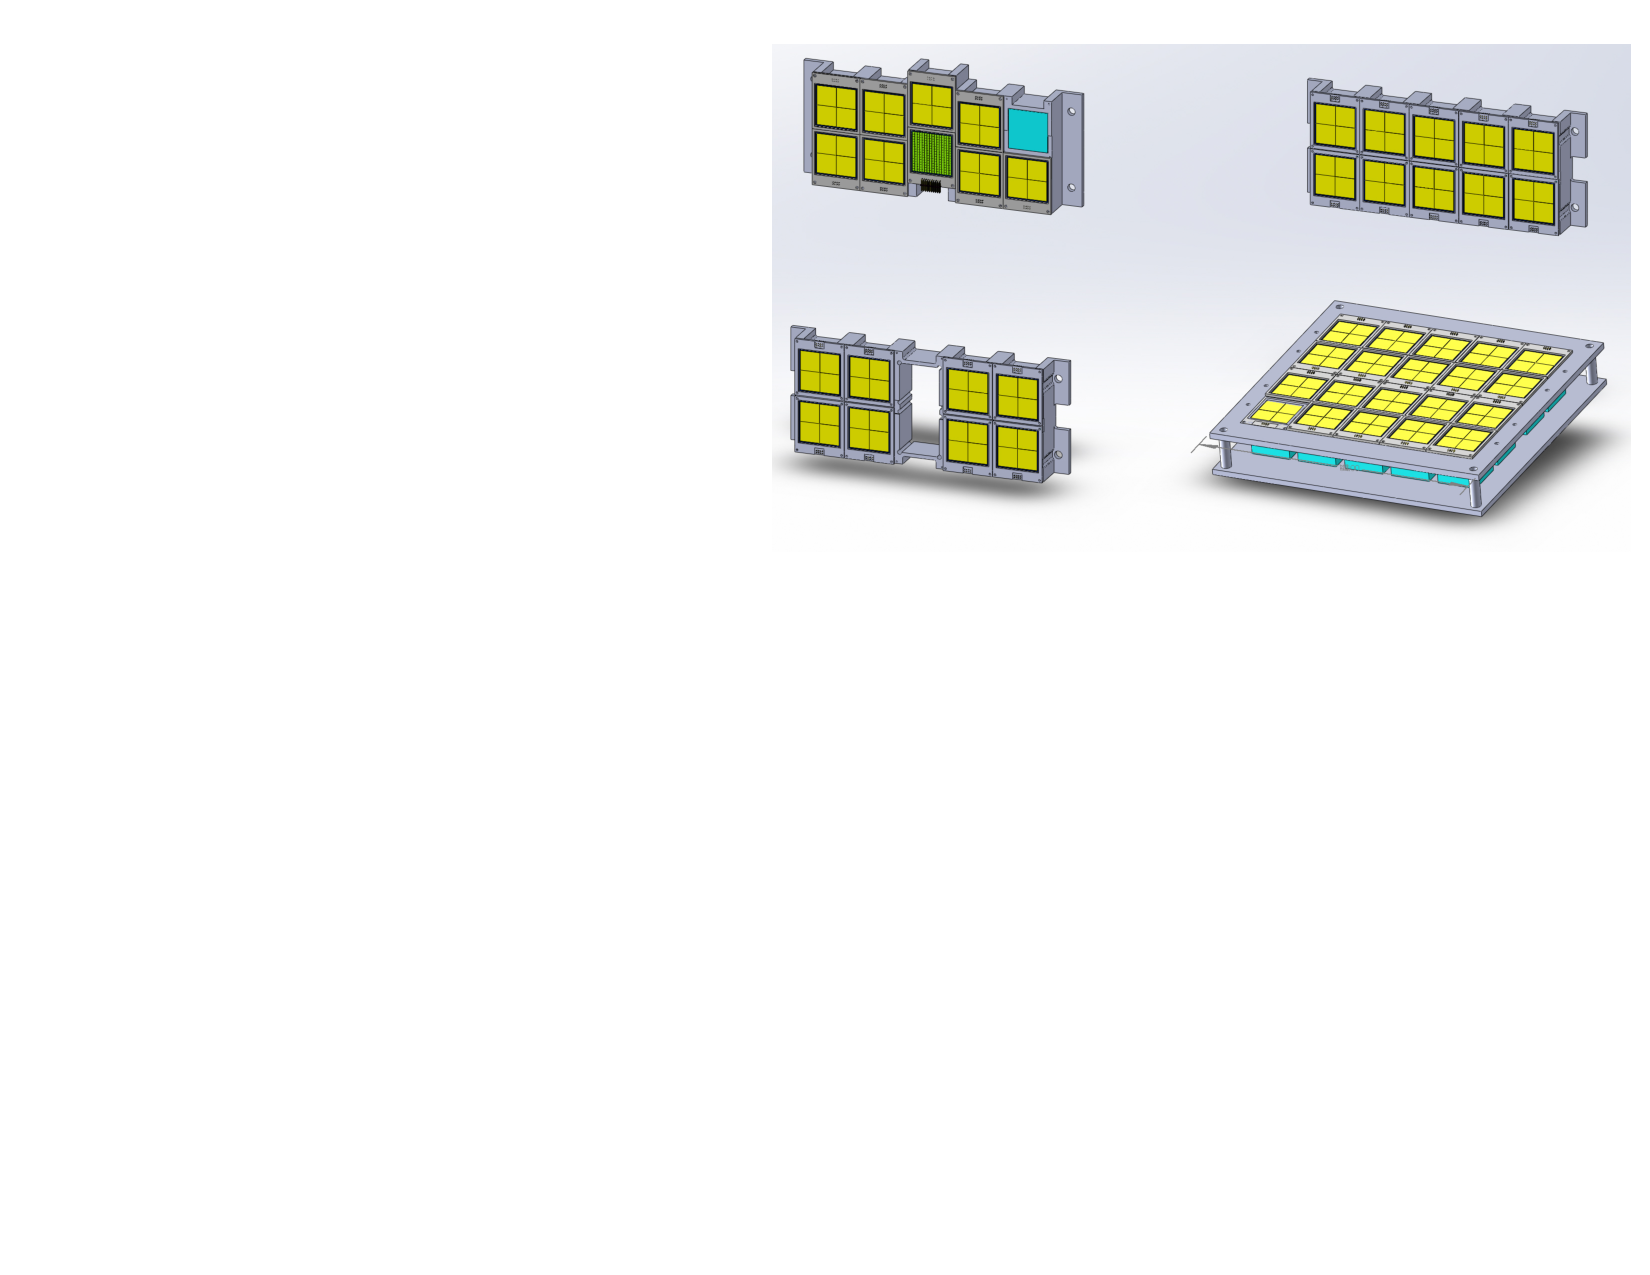
\includegraphics[width=1.0\columnwidth]{Figs/WallsAll}
    \caption{Rendering of the solid state telescopes of TexAT array: Forward array (top left); Side array (top right); Backward array (bottom left); Bottom array (bottom right). 
    One of forward Si- detector is removed to show an arrangement of CsI(Tl) scintillation detectors.} 
    \label{fig:WallsAll}
\end{figure}

Auxiliary detector systems, such as a windowless ionization chamber located at the entrance of the TexAT scattering chamber, right after the entrance window, and a scintillator located before the entrance window in vacuum have been used for some (but not all) TexAT experiments for normalization and beam diagnostics. These systems are not part of TexAT and will not be discussed further in this paper.

\subsection{Readout electronics \label{GET}}

The electronics channel count for TexAT is 1,024 channels for TPC readout, 232 channels for Si detectors and 58 channels for CsI(Tl) scintillation detectors, for a total of 1,314 channels. Readout electronics for all of these detectors is based on General Electronics for TPCs (GET). The details of GET system are published in Ref.  \cite{Pollacco}. Briefly, the TexAT readout system consists of 24 AGET chips. The AGET chip amplifies and shapes the signals while preforming pole-zero corrections. For each channel, the signal is stored in 512 time buckets (using switch capacitor arrays) with a frequency that can vary between 1 to 100 MHz (from 1$\mu$s to 10 ns per time bucket). The signals are compared to a threshold to provide a channel level trigger. Each AGET chip has 64 independent channels and include four extra channels to measure the noise. These ``noise'' channels are structurally identical to the 64 input channels and provide a way to subtract the electronic noise in the system.

The 24 AGET chips are installed onto 6 AsAd boards (4 chips per boards). The main role of the AsAd board is to digitize the signals from each AGET chip when a trigger is issued. The digitizer of the AsAd board is a four channel 12-bit ADC \cite{Pollacco}. Up to four AsAd boards can be connect to the top level of the GET electronics, the CoBo (\textbf{Co}ncentration \textbf{Bo}ard). When a trigger is sent to the CoBo board, the CoBo collects the data, time stamps the data and sends the data to be stored. An additional board called the MuTAnt (\textbf{Mu}ltiplicity \textbf{T}rigger \textbf{An}d \textbf{T}ime) is used to synchronize all of the CoBo boards. The MuTAnt board also collects the triggers from all of the CoBo boards and generates a global trigger. There are three different types of triggers in the GET system: Level 0, Level 1 and Level 2. The Level 0 trigger is an external trigger. A Level 1 trigger is done by summing the multiplicity triggers from the CoBos to generate a global trigger. The last trigger type, Level 2, can trigger on complex predefined pattern of channels that fired. The Level 2 trigger has not been tested with TexAT yet.

\subsection{Transition ZAP- boards}

To connect detectors  to the AsAd cards, a special readout  adapter  boards (referred as ZAP) have been designed for each kind of detectors (MM, Si- and  Csi(Tl)). ZAP- board allows to readout signals from the detectors, to bias them (individually or in groups) and  to protect sensitive electronics of AsAd cards and AGET chips from the electrical  breakdown caused by potential sparks in Micromegas detector. 

\subsubsection{Micromegas ZAP- board design}
The  basic circuitry for the signal readout allowing protection, suggested by developers of GET electronics is shown in Fig. ~\ref{fig:MMZAP_circuit} (\cite{GET}). The protection circuitry is based on a diode bridge. A "common mesh" circuit  is used for TexAT's  Micromegas detector: pads/strips/chains were set at positive DC potential  (200 to 600 V) to create an avalanche in Micromegas detector. Such approach allows to set tension individually at different zones of TexAT Micromegas detector (see Sec. \ref{lowANDhigh}) to create avalanche areas with different gas gain. The board-to-board connection concept was used to reduce noise and to avoid eventual connection problems with high density cables between electronic components. Every Micromegas ZAP card has 4 individual biasing lines through the LEMO- connector (shown on the left in Fig. ~\ref{Fig:ZAP_All_Crop}). In later ZAP- board release the LEMO connectors were replaced with the high voltage rated SHV- connectors to ensure functioning at the higher tension ($>400$ V). Micromegas ZAP "input" interface matches to MM readout board interface (SAMTEC male/female) and ``output'' ZAP- interface matches to AsAD card interface (SAMTEC female/male). Such board-to-board connection concept allows to reduce noise and to avoid eventual connection problems with high density cables between electronic components.

The micromesh is either grounded or fed to the charge sensitive preamplifier (Canberra). In latter case, the signal from the mesh can be monitored with an oscilloscope or/and to be used to generate a trigger.

\subsubsection{Si- detectors ZAP- board design}

ZAP- card for readout signals from Si-detectors is shown in the center  in Fig. \ref{fig:ZAP_All_Crop}. For the purpose of unification of readout electronics the protection part of ZAP has been maintained, even though a Si- detector is a unity gain device and no spark damage is expected. ZAP card  consists of four identical group of channels, each one maintains up to 16 x 4 quadrant Si detectors ( MSQ25-1000 or KDP-1K, 64 total individual channels). The  Si-detectors connected to ZAP board inside scattering chamber by flat cables combining 8 detector outputs to 32 ribbon cable,
plugged to standard 34 pin header (as can be seen on the bottom of central part in Fig. ~\ref{fig:ZAP_All_Crop}. 
The readout circuitry of Si- detectors is similar to the one, shown in Fig. ~\ref{fig:MMZAP_circuit}, but the serial circuit of  (1M - 10M) resistors 
is used instead of (10M - 100M). Detectors are biased through the 16 position connector header, a single bias line supports 4 Si detector front channels.
In full configuration TexAT consists of 58 Si-detectors. The current ZAP-board configuration allows to read out signals from "Front"- side  of all detectors
provided that "Backs"- of all detectors are common. The signals from the back side of Si-detectors can be also readout, but in this case 
the total number of detectors is limited to 48 (single AGET is not able to work with "mixed" polarity signals).  All Si detectors are biased from MPOD Power supply unit. 


\begin{figure}[hbt!]
    \centering
     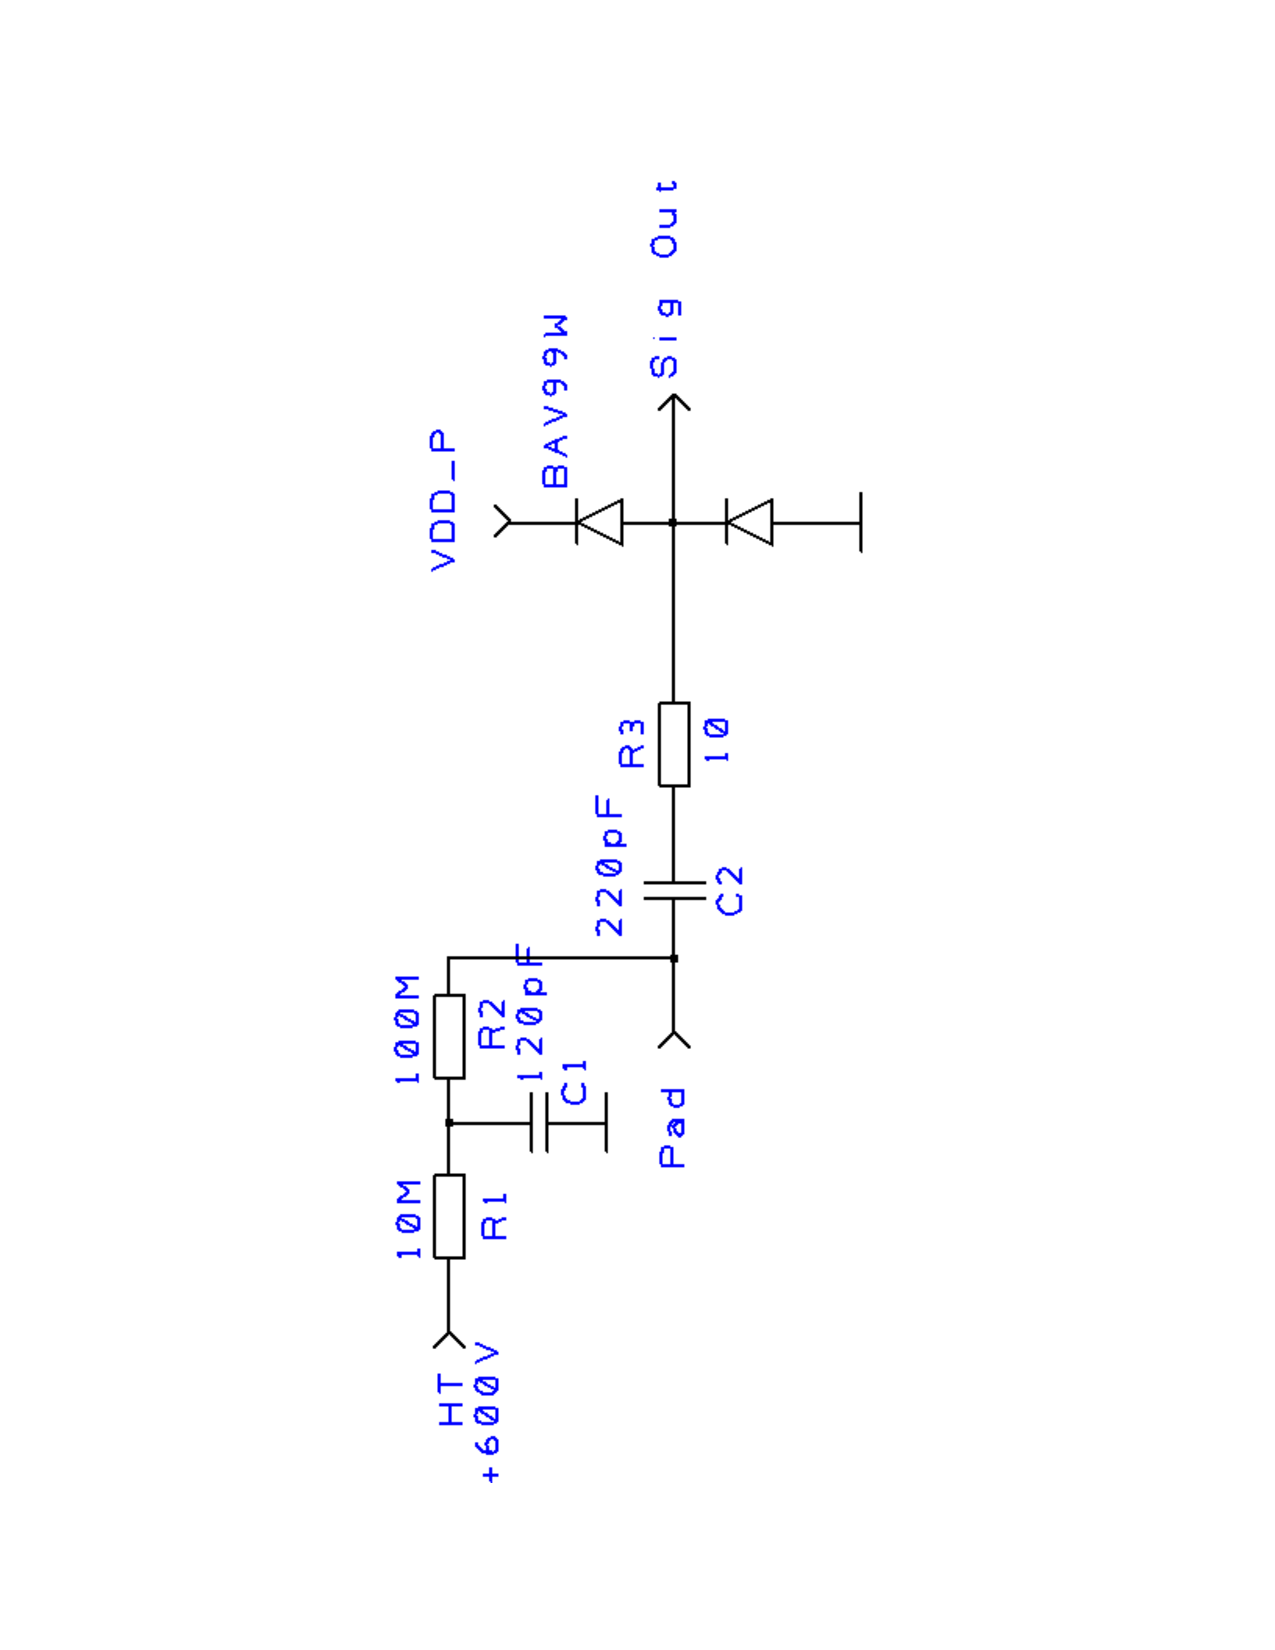
\includegraphics[width=0.8\columnwidth, angle=270 ]{Figs/Micromegas_ZAP_Circuit.pdf}
    \caption{Micromegas readout and protection circuit schematic}
      \label{fig:MMZAP_circuit}
\end{figure}


Signals from the detectors go through the SAMTEC connectors to the internal AGET preamplifier. 

Scintillation detectors ZAP design:

Signals from the CsI(Tl) scintillation detector were output of its own custom preamplifier, located right to the PIN diode to reduce the electronic noise. This negative voltage output lead us to bypass an integrated Charge Sensitive pre-Amplifier (CSA) function and filter stages of the AGET chip. In addition, the "slow" output of the detector required an optimal peaking time of 4 to 6~$\mu$s, while the available range of peaking time for the AGET chip extends  from 50 ns to 1 $\mu$s (sixteen values total). In order to optimize the signal processing of the detector, it have been decided to use a 16-channel  MESYTEC  shaper (MSCF-16)~\cite{MESYTEC} and feed properly the shaped output signals into an Inverting x2 Gain (G-2) function of the AGET chips (See \cite{GET} for details). The G-2 stage provides an extra inverting voltage gain and a buffering for signal sampling in a Switch Capacitor Array (SCA) in the AGET chip. The offset voltage of the Gain-2 input signal was adjusted by the non-inverting level shifter circuit with the 75~MHz gain bandwidth LM6154BCM Operational Amplifier (OpAmp)~\cite{OpAmp} (Fig. ~\ref{fig:CsIZAP_circuit}), depending on the polarity of input signals: +2.2~V for positive polarity or 0.7~V for negative polarity.
%LM6154BCM/NOPB data sheet in https://www.ti.com/lit/gpn/LM6154

\begin{figure}[hbt!]
	\centering
	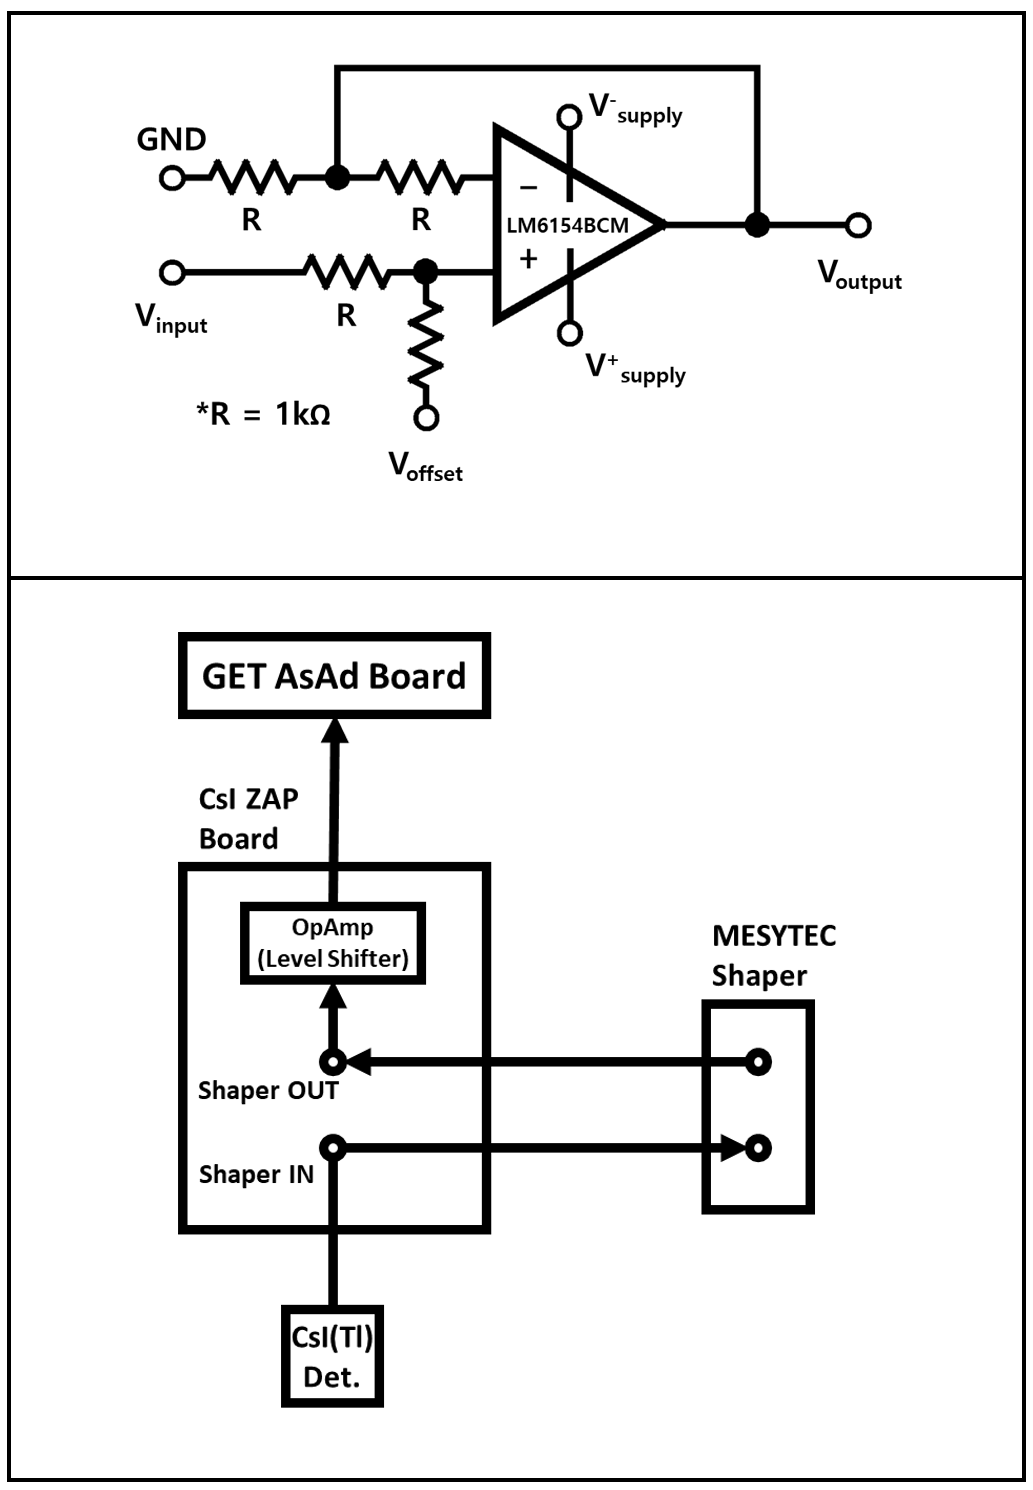
\includegraphics[width=1.0\columnwidth]{Figs/CsIZAP_circuit}
	\caption{Top: A schematic of the non-inverting level shifter circuit using the LM6154BCM OpAmp. The supply voltage, V$^{+}_{supply}$ or V$^{-}_{supply}$, was adjusted to match an impedance of the circuit and GET electronics input. Bottom: A signal processing diagram using the external shaper for CsI(Tl) scintillation detector.}
	\label{fig:CsIZAP_circuit}
\end{figure}
 
The custom ZAP board has been designed. The sixteen total fast OpAmp integration circuits were implemented on the board. While one offset voltage and one supply input can be set for all the OpAmp circuits, one OpAmp handles 4 independent channels resulting in 16 outputs for each AGET chip input corresponding to the full channel numbers of one MESYTEC module. One ZAP board allows us to process signals from 64 total CsI detectors, placed inside the TexAT chamber.

The PCB design was made using prototyping software  Design Spark PCB 7.1~\cite{DesignSpark}. The boards are 4 layers and all elements are surface mounted.  
 All electronic components are placed outside of TexAT scattering chamber to simplify the replacement in case of electronic failures. All
  ``Transition"-  board have a similar form- factor. They are  epoxi- sealed to the custom vacuum flange, making a signal feed-through 
  to the TexAT scattering chamber.  

The photo image of all ZAP- boards is shown in  Fig. ~\ref{fig:ZAP_All_Crop}.
		                                       
\begin{figure*}
    \centering
     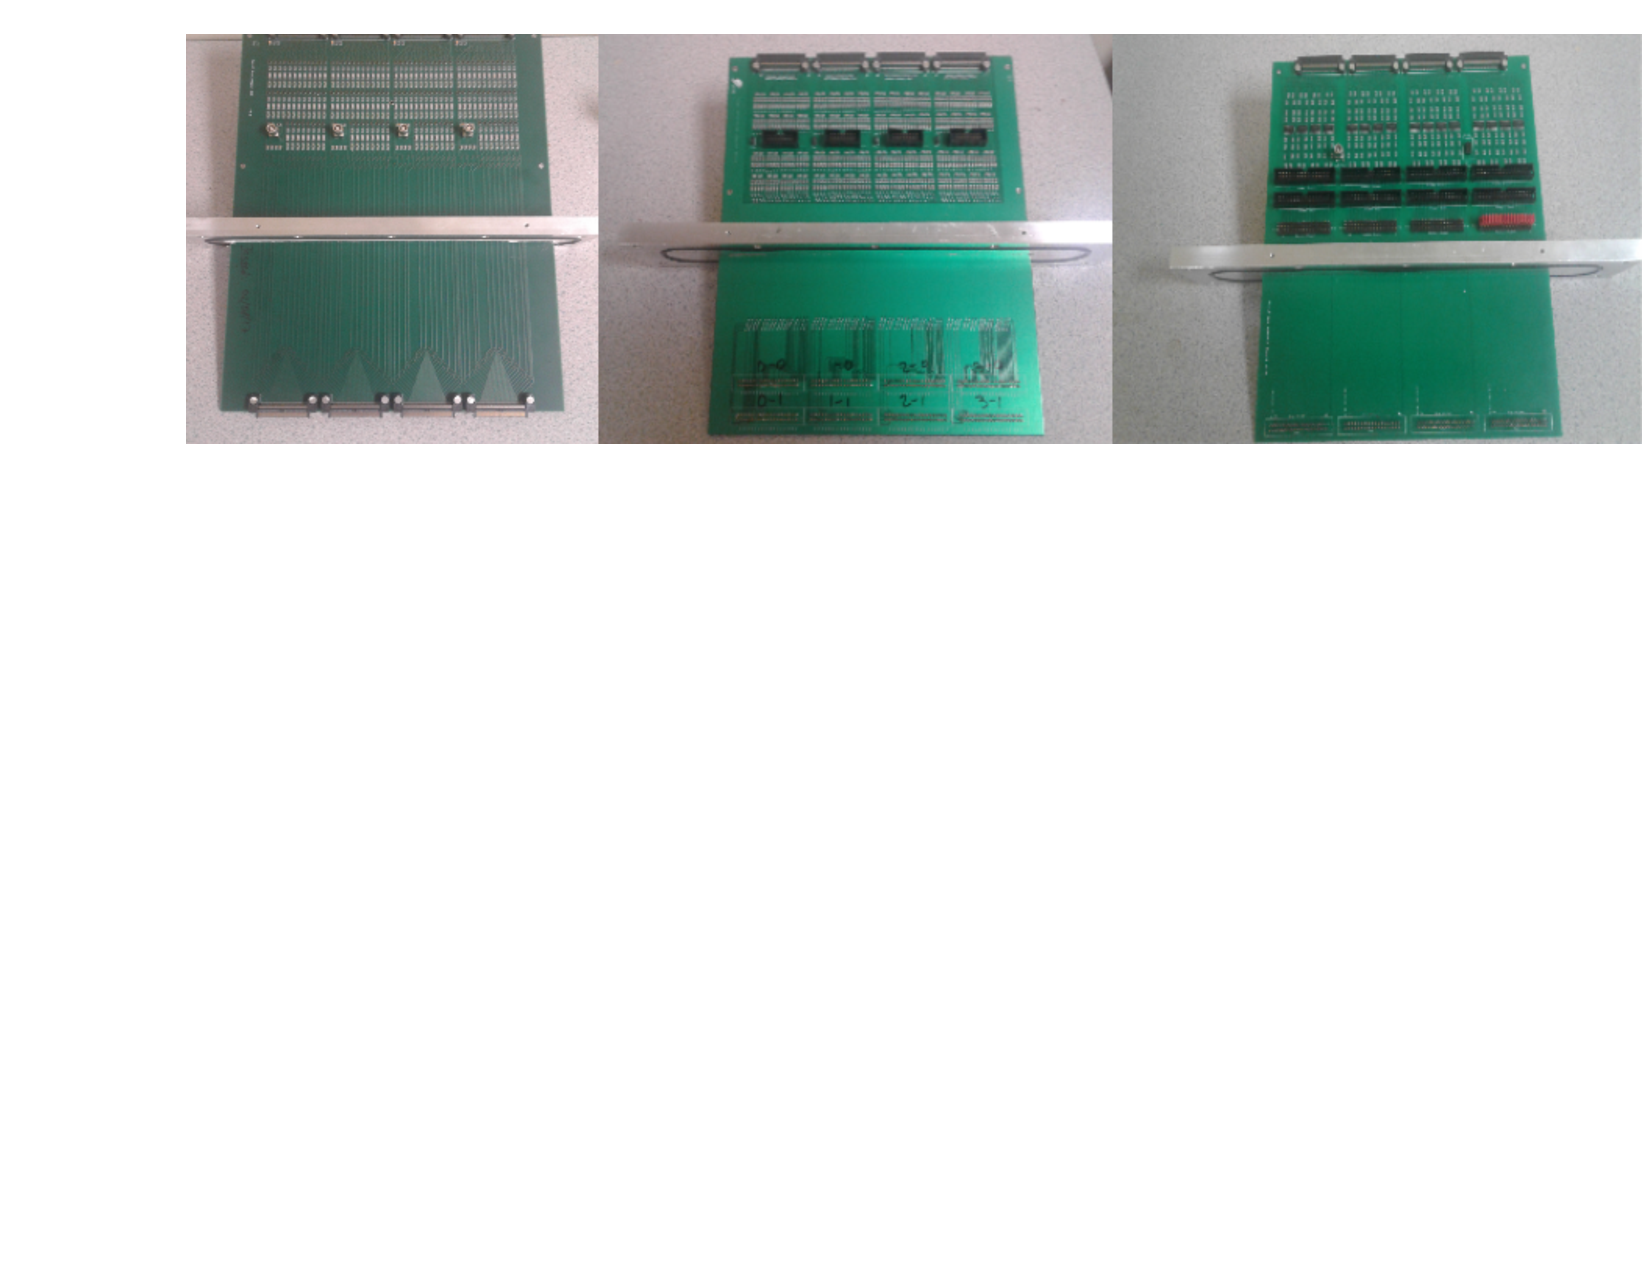
\includegraphics[width=\textwidth]{Figs/ZAP_All_Crop}
    \caption{Micromegas ZAP boards: Left: MM; Center: Si; Right: CsI}
      \label{fig:ZAP_All_Crop}
\end{figure*}

\subsection{Scattering Chamber}

A custom scattering chamber  has been designed to hold the detector array and to maintain the workable conditions for both gaseous (Micromegas and ion chamber) and solid state (silicon and scintillation) detectors. It has an aluminum body/shell of cuboid shape: 20in x 20in x 13.5in, made from 1 inch thick aluminum sheet. The top cover is designed to secure a Micromegas based time-projection counter (TPC). It also has six slots for vacuum feedthroughs (ZAP-boards) to read out the anode signals from  Micromegas and solid state (semiconductor and scintillation) detectors. All readout electronics is coupled directly to the feedthroughs, eliminating cables. 
	
Each of four chamber's sides has a square (14 inch by 8 inch) port, plugged with a O-ring's vacuum sealed doors. Such design allows to mount solid state detectors, surrounding the TPC at each flange independently. It provides  an easy access to  all components of detector array and  versatile installation at any beam line (either at in-flight exotic secondary beam line using MARS- separator,  or at future project of re-accelerated exotic beam line) through the standard ISO-100 upstream vacuum flange.  	A scattering chamber's gas volume is separated from the beam line with a thin vacuum tied Havar/Kapton/Mylar entrance window with the diameter of 12.5 mm,  mounted at the forward wall, connecting  TexAT to the beam-pipe.
	
A small  planar windowless Ion Chamber (IC) with a Frish grid can be mounted at upstream flange. IC works in  the same target gas media to provide a particle ID and count ions of incoming beam. IC  provides additional normalization and beam-tracking capabilities.
	
The bottom side of the chamber is equipped with ISO-100 compatible style port for vacuum pumps connection. 
Another set of KF40 ports is placed at side walls (2 at each wall, 8 total). These ports are used for gas inlet/outlet, Vacuum/Pressure/Temperature-  sensors,  IC voltage/readout  and high voltage feedthroughs, supplying different circuits. 

Chamber finish is mechanically polished and deionizied to meet the pretty narrow requirement for  steady operation of  sensitive to impurities Micromegas  detector. The chamber tested at leak rate in the range of 10$^{-8}$ atm-cc/sec.

\subsection{Gas handling system}
	
The multipurpose vacuum and gas handling system
has been developed to provide a possibility of running experiments with
exotic beams in both "detector" (for example, decay- experiments)  and "active target" (resonance scattering,
transfer reactions, etc.) modes. It is similar to those, we built for ANASEN detector \cite{}.
The gas pressure and flow is controlled by  an integrated pressure
controller with mass flow meter $\pi$PC-99 from MKS Instruments.
It can control gas  pressure through
TCP/IP protocol at the range of 15 Torr to 1250 Torr  with the accuracy of $\pm$1\%.
System was tested for gases like Helium/CO$_2$ mixture, Carbon Dioxide, Argon and mixtures (P5/P10).
It also meets  safety specifications for use of flammable gases (Hydrogen/Deuterium, Methane,
Iso-butane, etc.) and it was tested with those gasses as well.

The reliability of the system has been demonstrated during several 3 - 4 week long runs.
	
\section{Micromegas Simulation}

The complete TexAT Monte Carlo simulation package was developed. These simulations utilized the Geant4 \cite{Geant4} and Garfield++\cite{GARFIELD} libraries. Two reactions were studied as the test case: $^{12}$C(p,p)$^{12}$ and $^{18}$Ne($\alpha$,p)$^{21}$Na. In the latter, residual $^{21}$Na nuclei in both the ground state and first excited state were populated. In the simulation, the incoming ions were forced to undergo the reaction of interest at a random point within the TPC using realistic reaction kinematics. At each step of an incoming or product track, the total ionization energy was converted to a number of electron and ion pairs, and each electron was drifted under a constant electric field to the MicroMegas board. Time-dependent histograms of the number of detected electrons for each pad of the MicroMegas board were generated and stored for offline processing. Additionally, the energy collected in each detector of the Silicon array was also recorded per event. Fig. ~\ref{fig:Simulation_1} shows an example event visualized in Geant4.
	
	\begin{figure}[hbt!]
    \centering
     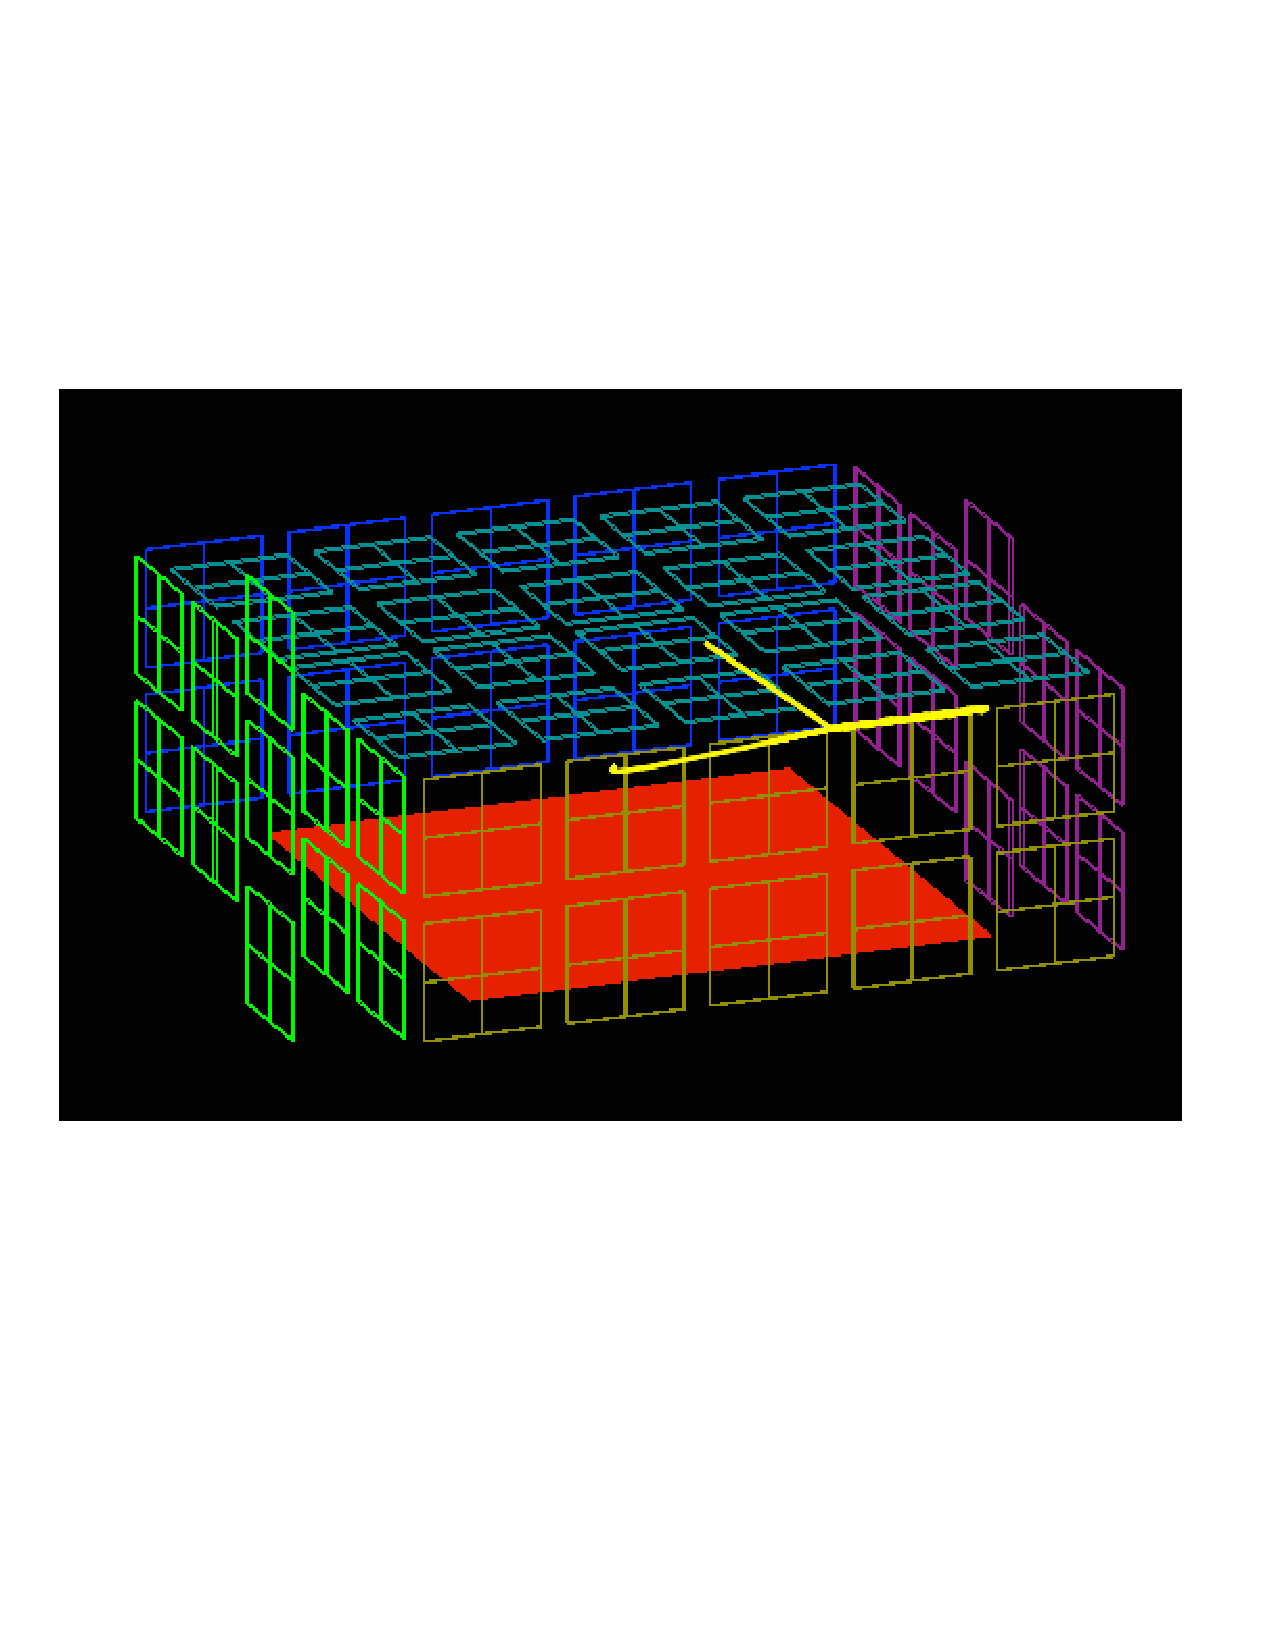
\includegraphics[width=1.0\columnwidth]{Figs/Simulation_1}
     \caption{Example of simulated track for the $^4$He($^{18}$Ne,p)$^{21}$Na reaction in the TexAT detector as visualized in Geant4. The light recoil (proton) hits the Si detector on the top plate and the heavy recoil ($^{21}$Na) stops in the gas volume.}
     \label{fig:Simulation_1}
   \end{figure}

	
Custom track reconstruction routines have been developed for the TexAT detector. For
particles traversing the left and right regions, X-Y coordinates are determined by matching strips
to chains (or vice versa) using the average recorded drift time. In the central region, the X-Y
coordinates of a track are determined solely from the position of the rectangular pad with the
highest electron count per row. Such a procedure yields two tracks: one for the light product and
one combined track for the incoming ion and heavy recoil. By finding the point of closest
approach of the fitted light product and the heavy ion tracks, the heavy ion track in the central
region can be split into separate incoming and recoil tracks. Finally, the three tracks are re-fit
simultaneously to find the vertex of the interaction and the relative angles of the reaction products. 
Fig. ~ \ref{fig:Simulation_1} shows an example of the track reconstruction. 

\begin{figure}[hbt!]
    \centering
     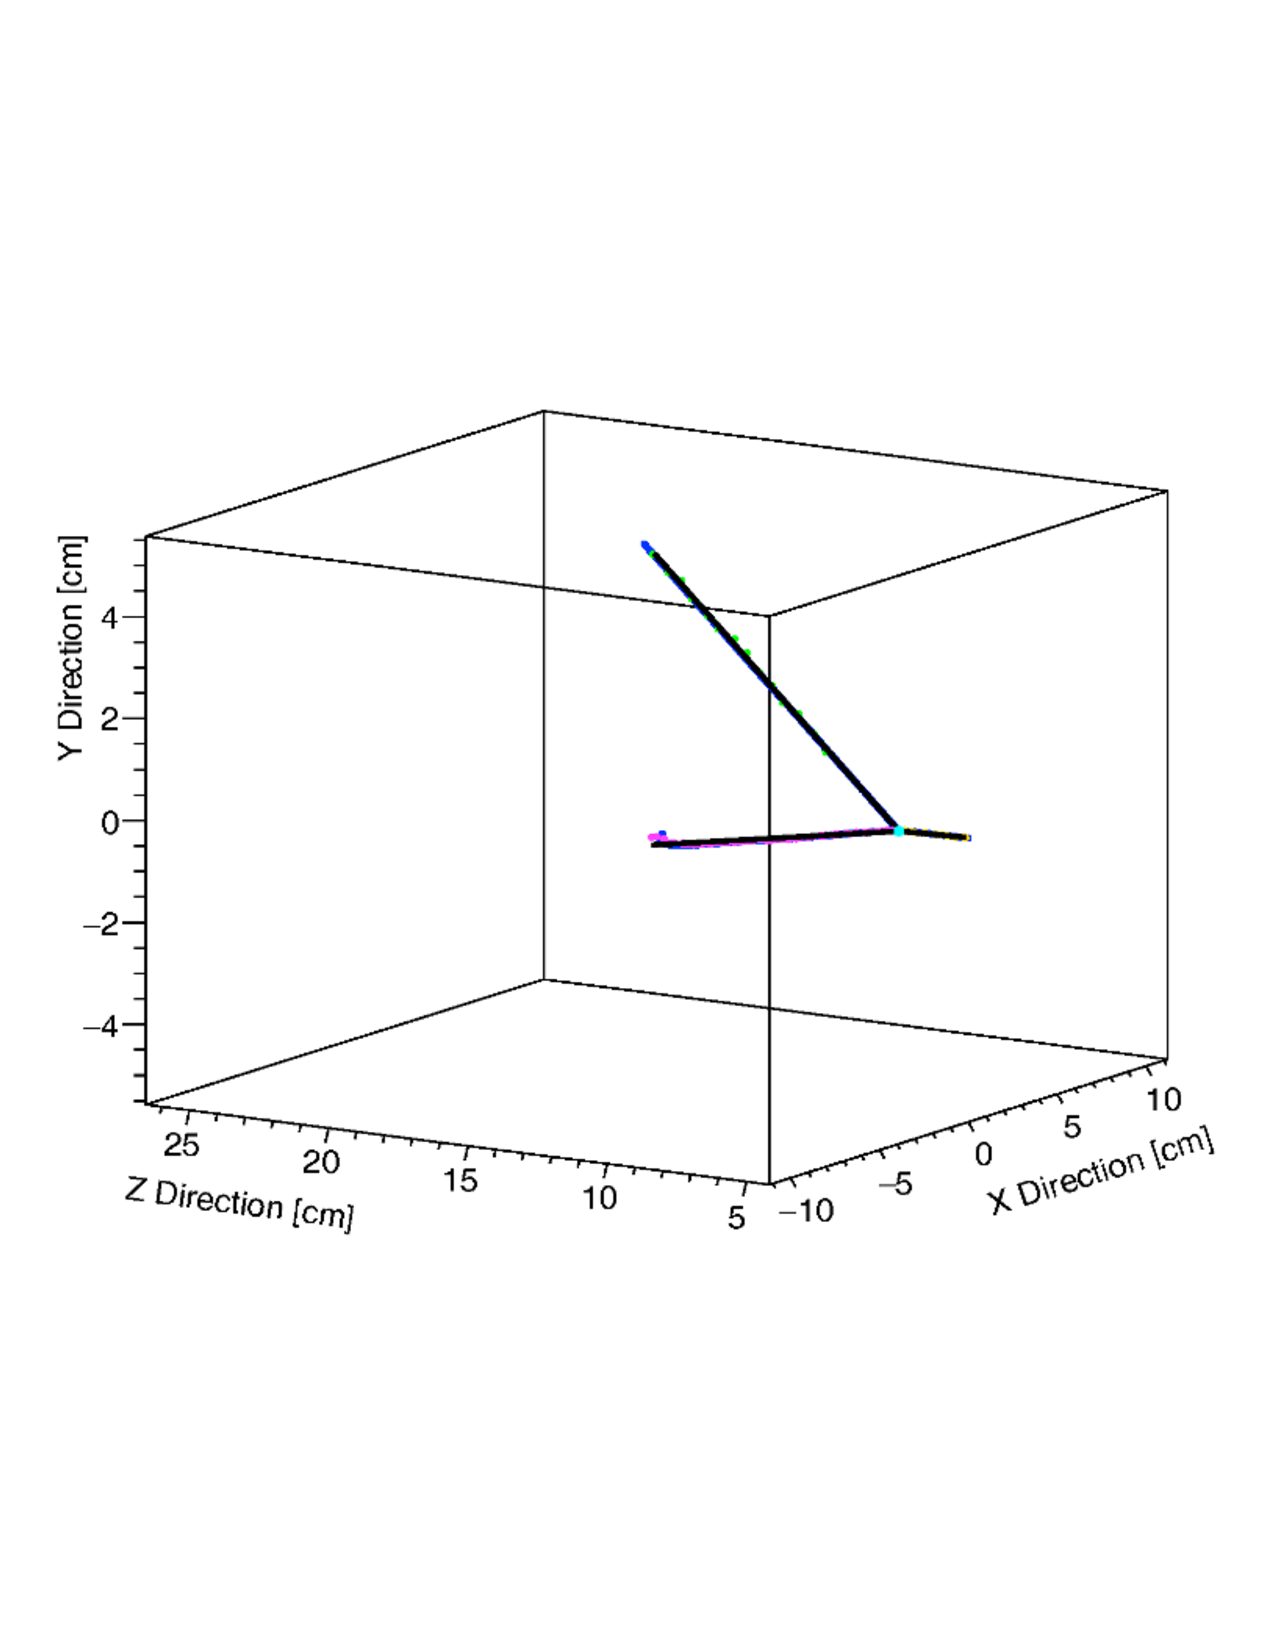
\includegraphics[width=1.0\columnwidth]{Figs/Simulation_2}
     \caption{Same track as in Fig.~\ref{fig:Simulation_1}, but reconstructed from drifted electrons
detected by the MicroMegas pads.}
     \label{fig:Simulation_2}
   \end{figure}

The blue points are the simulated interaction points, while the yellow, purple and green points are reconstructed from the
information recorded from the simulation for the MicroMegas board. The black lines are the
fitted tracks, and the teal point indicates the fitted reaction vertex. For the reactions of interest,
the vertex reconstruction error was found to be approximately 1.5 mm on average, with a
distribution that peaked below 1 mm. The angular resolution determined from the simulation was
approximately 3$^{\circ}$ at FWHM. If the Q-value of the reaction is unknown, the center of mass
information recorded from the simulation for the MicroMegas board. The black lines are the
fitted tracks, and the teal point indicates the fitted reaction vertex. For the reactions of interest,
the vertex reconstruction error was found to be approximately 1.5 mm on average, with a
distribution that peaked below 1 mm. The angular resolution determined from the simulation was
approximately 3 degrees at FWHM. If the Q-value of the reaction is unknown, the center of mass
energy of the interaction can only be reconstructed from the vertex position and the average
energy loss in the gas, and is limited by energy straggling effects. For the incoming $^{18}$Ne ions,
this yielded a center of mass energy resolution of 190 keV at FWHM. Using the interaction
energy as provided by the vertex, in addition to the angle and energy (measured in Si detectors) of
the light product, the Q-value can be reconstructed. In the case of the $^{18}$Ne($\alpha$,p)$^{21}$Na reaction,
transitions to the ground and first excited states of $^{21}$Na (separated by only 330 keV) could be
well resolved (see Fig.~\ref{fig:Reconstruction_1}). (Assuming that energy resolution of the incoming $^{18}$Ne 
beam corresponds to the ``typical'' energy resolution of reaccelerated radioactive beams.)

\begin{figure}[hbt!]
    \centering
     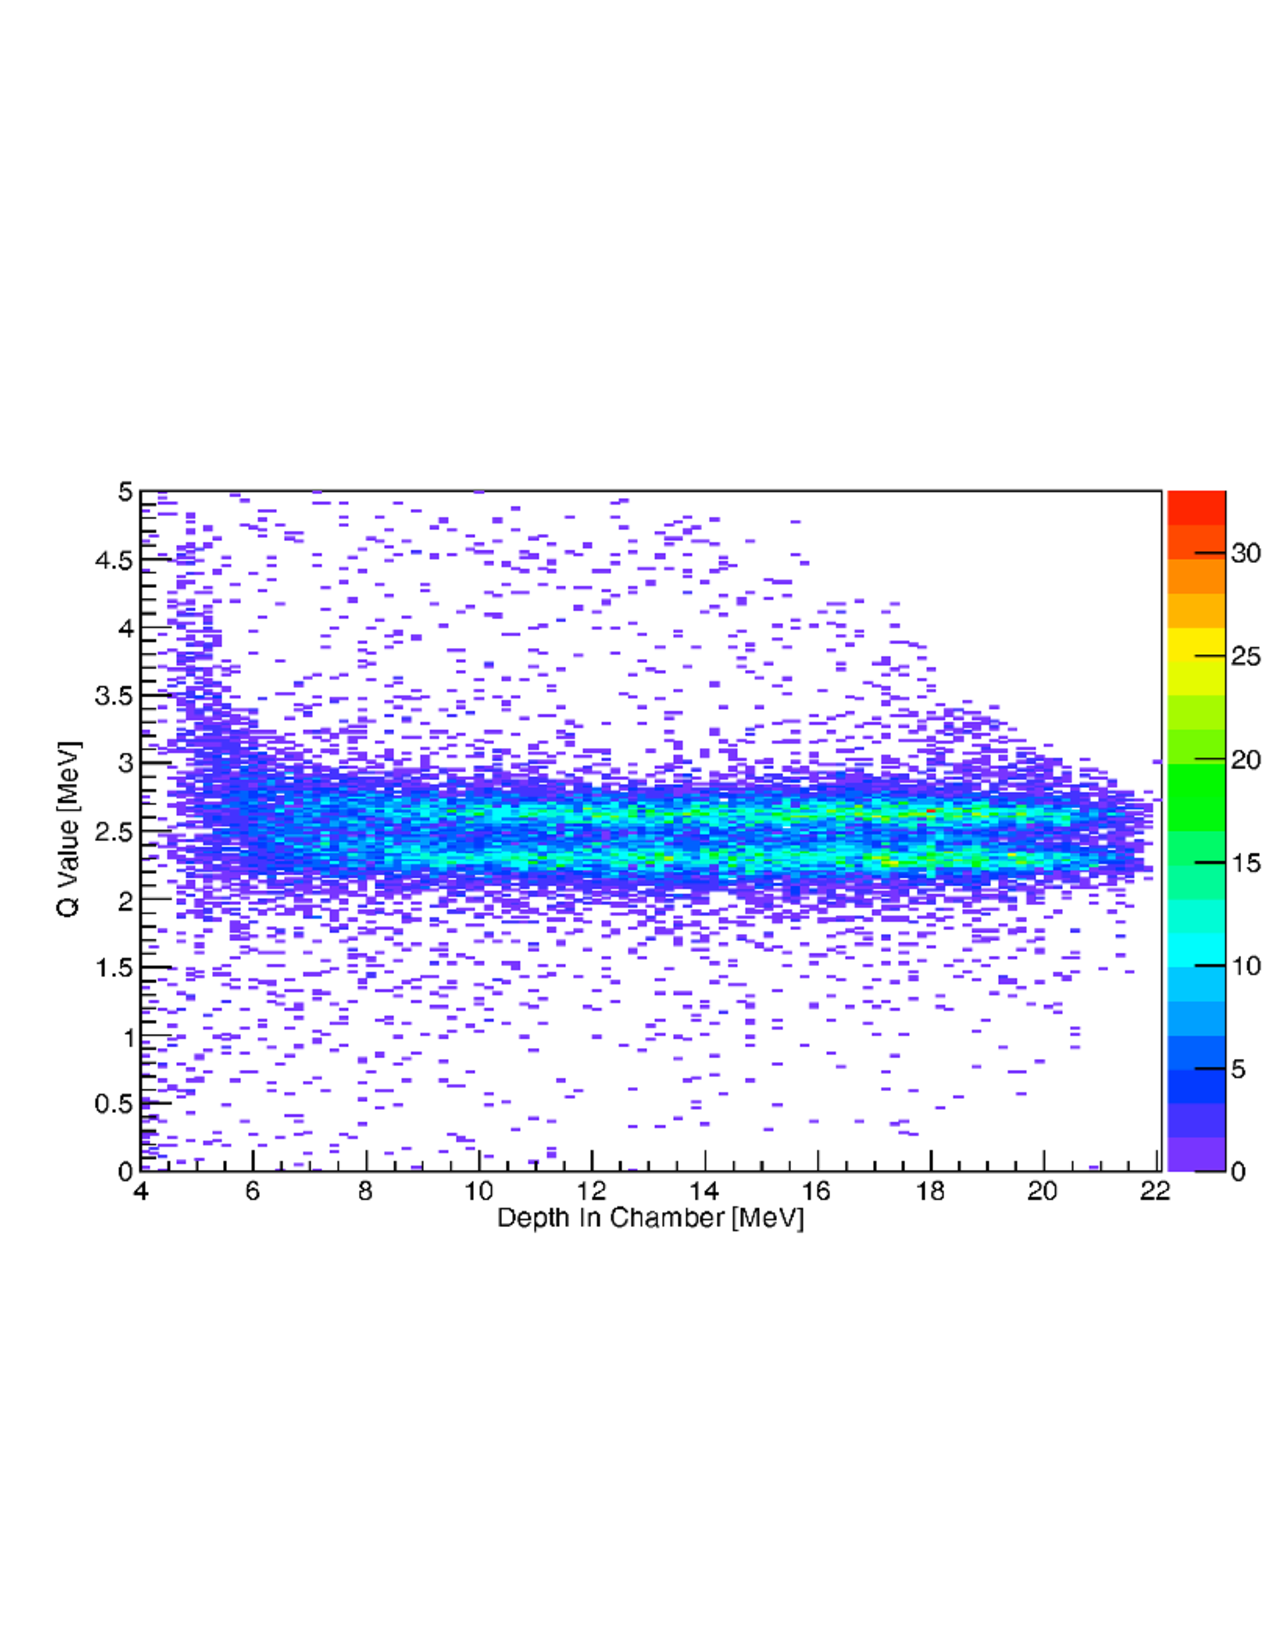
\includegraphics[width=1.0\columnwidth]{Figs/Reconstruction_1}
     \caption{Reconstructed Q-value vs. chamber depth for the simulated $^{18}$Ne($\alpha$,p)$^{21}$Na reaction}
     \label{fig:Reconstruction_1}
   \end{figure}


Once the reaction mechanism is identified (e.g. elastic or inelastic scattering), the c.m. energy resolution can be improved by recalculating using the Q-value, the detected energy in the Si detector, and emitted light product angle. In the present study, the center of mass energy resolution for these events was found to be 40 keV at FWHM (see Fig. ~\ref{fig:Reconstruction_2}).
		
\begin{figure}[hbt!]
    \centering
     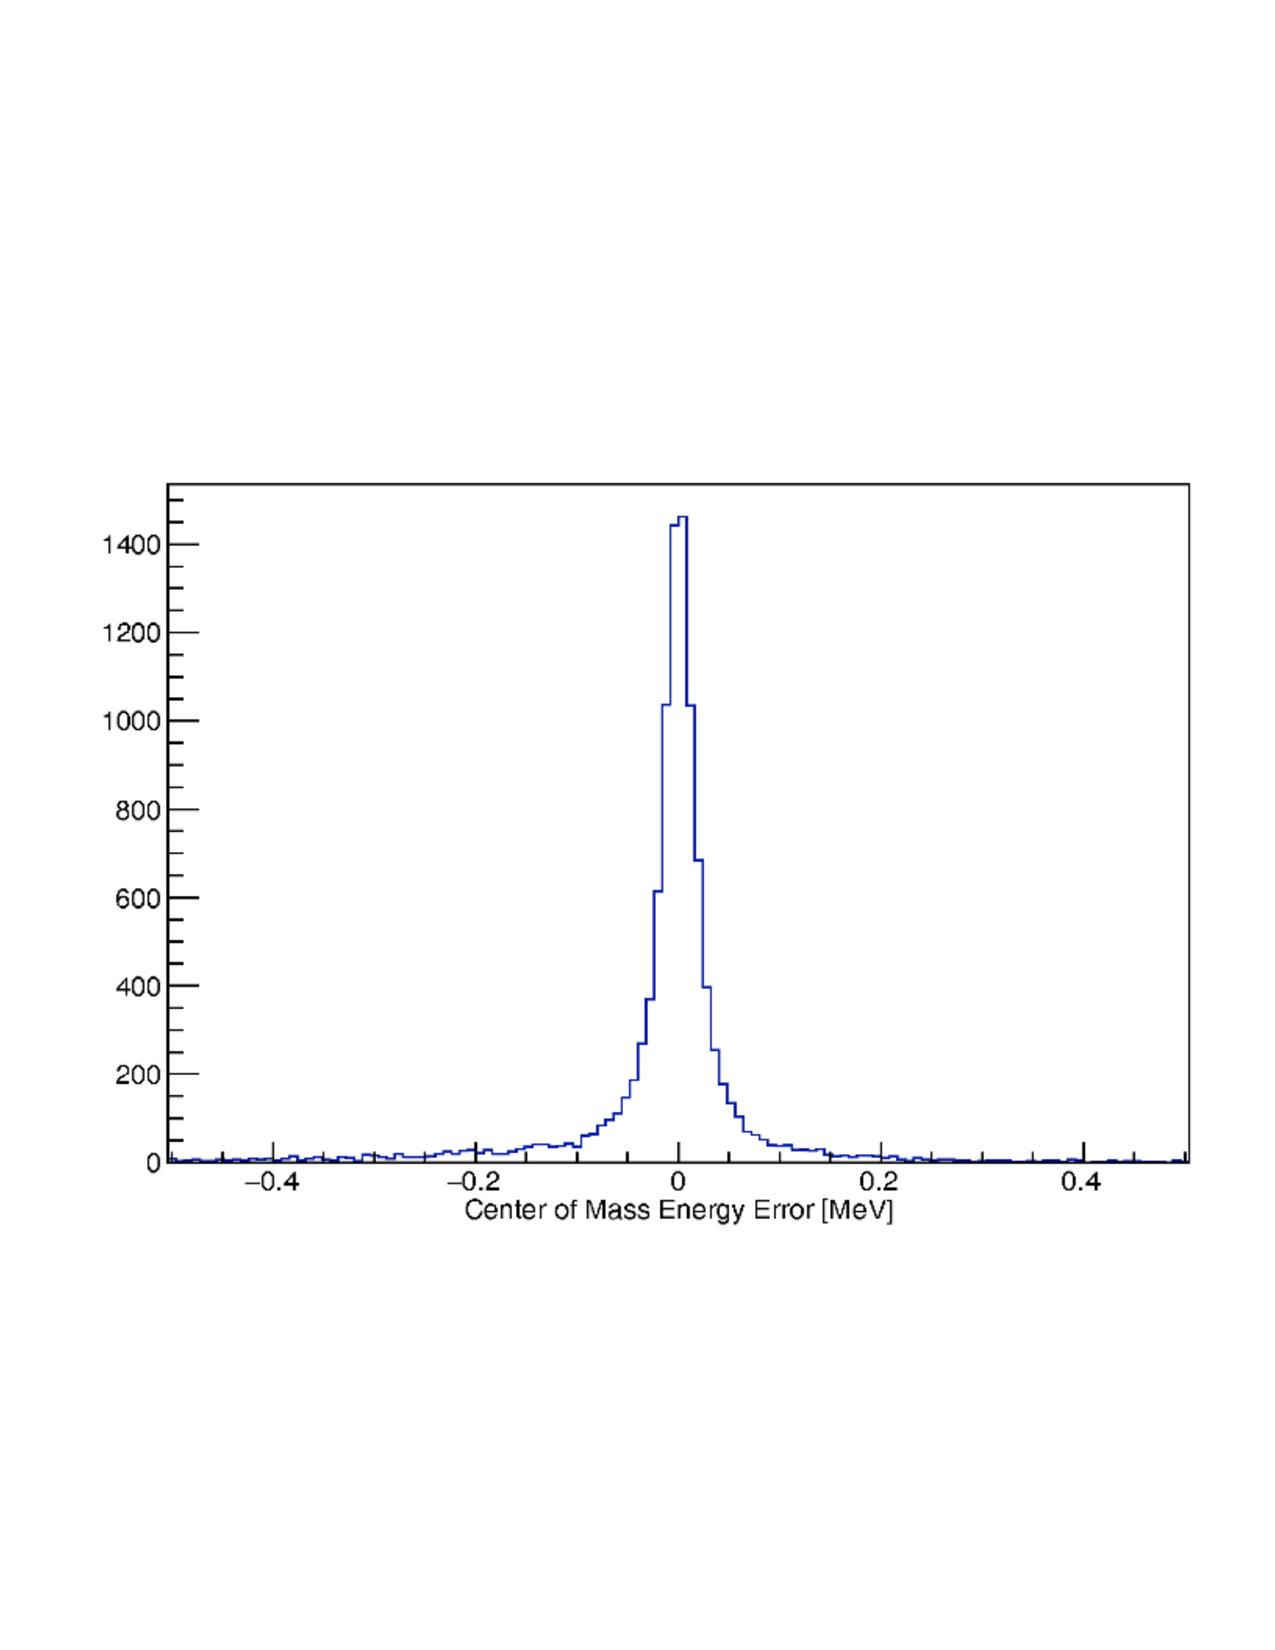
\includegraphics[width=1.0\columnwidth]{Figs/Reconstruction_2}
     \caption{Center of mass energy resolution for the simulated $^{12}$C(p,p) $^{12}$C reaction.}
     \label{fig:Reconstruction_2}
   \end{figure}

Additionally, these energy and angle resolutions were found to be mostly insensitive to the depth within the scattering chamber and therefore interaction energy and scattering angle. The simulations demonstrate that the segmentation implemented in TexAT is sufficient to reconstruct the observables with high enough precision to identify the events due to population of two closely spaced excited states ($\sim$300 keV) in the ($\alpha$,p) reaction. It was shown that track reconstruction allows for energy resolution of 40 keV and angular resolution of $\sim$3$^{\circ}$ over wide range of excitation energies and scattering angles.

\section{Data Analysis}

The analysis of the data recorded using the GET DAQ with the TexAT detector involves a multi-step process. It involves subtraction of the baseline for all signals, the wave form fitting to determine waveform maximum amplitude values and peak times, matching chains and strips in the side region to create three-dimensional points for track reconstruction and fitting tracks using various methods for noise reduction.

\subsection{Baseline Corrections and Obtaining the Energy and Timing}

The AGET chips have 64 input channels but provide 68 output channels. Four of these channels are called fixed-pattern noise (FPN) channels that are not connected to any detector and record the intrinsic noise and electronic baseline \cite{Pollacco}. These four channels are averaged together and subtracted from each waveform of the remaining 64 channels to remove the intrinsic noise in the electronics. Examples of the FPN channels and raw waveforms are shown in Figure \ref{fig:FPN_Raw}.

\begin{figure}[hbt!]
  	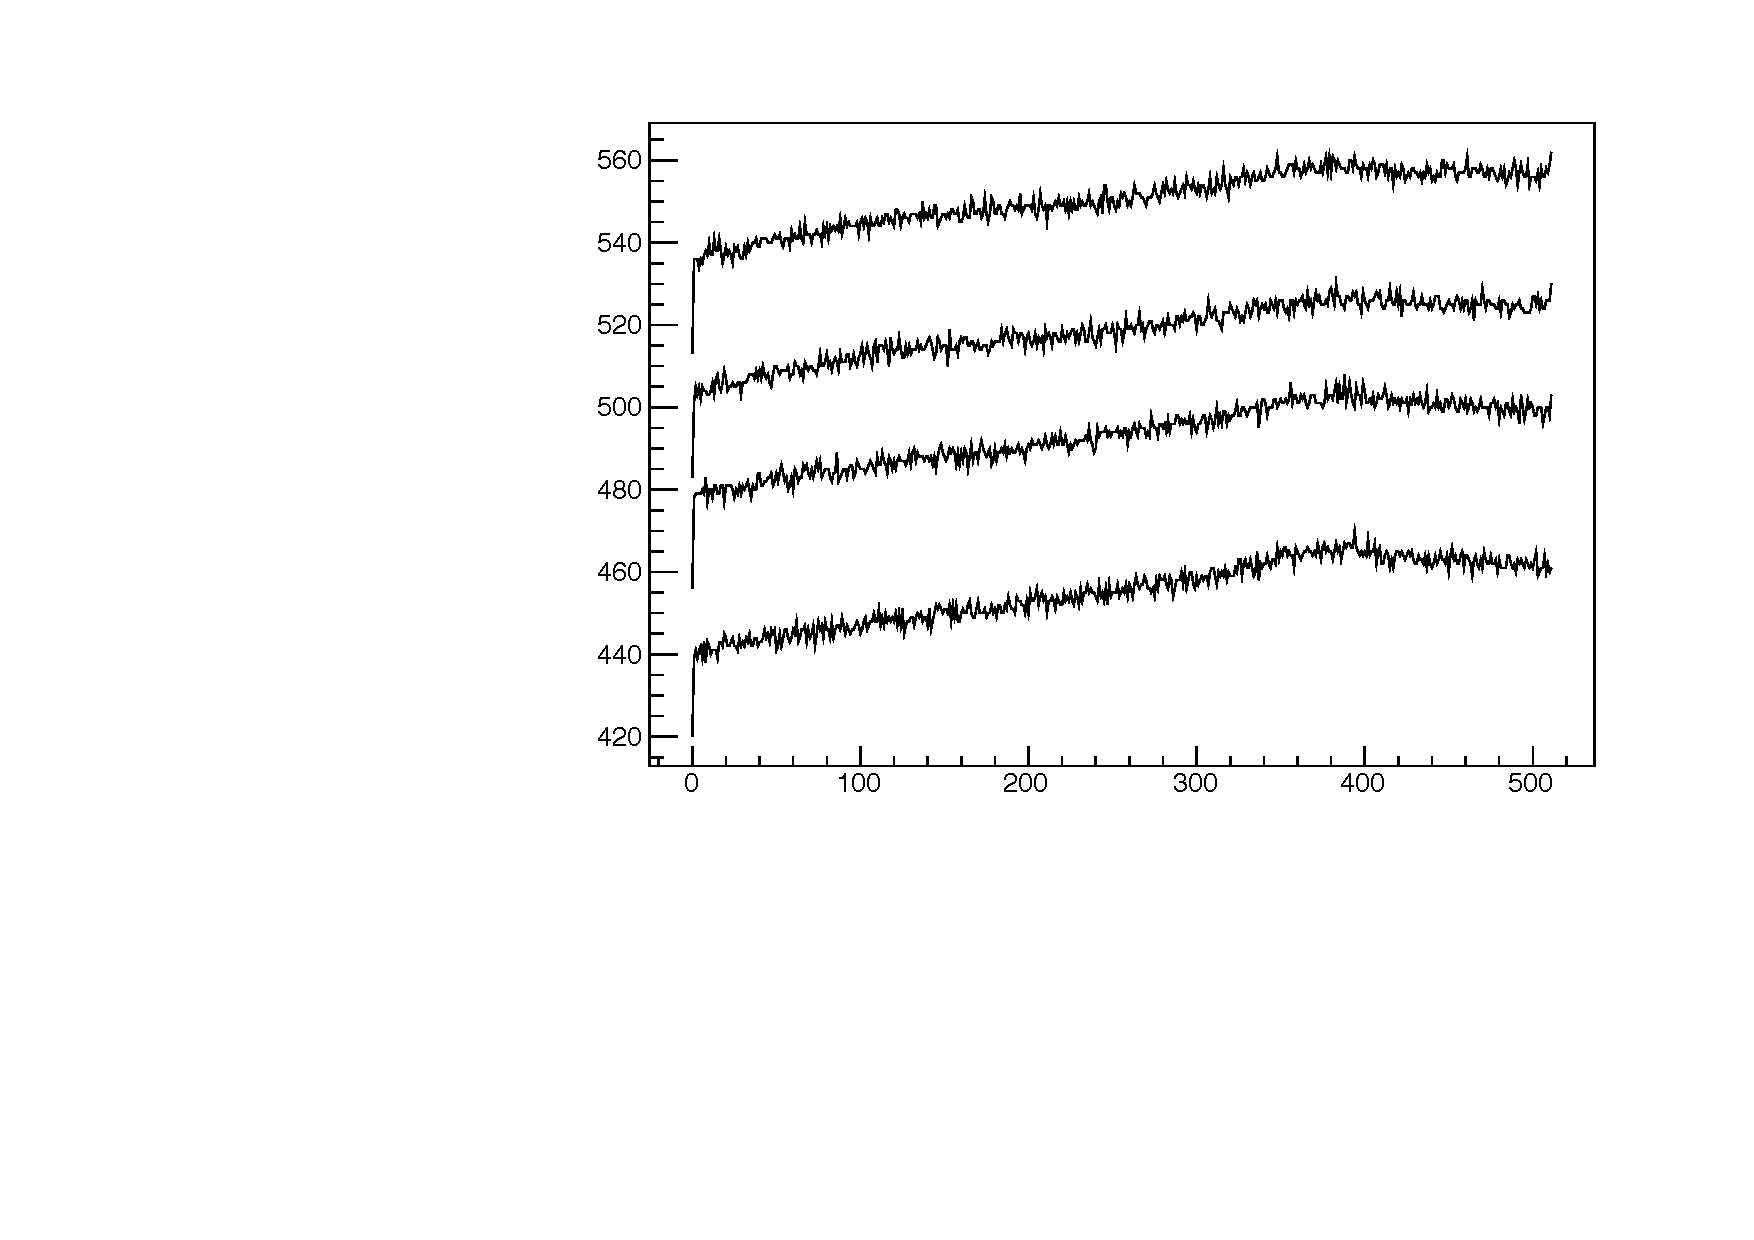
\includegraphics[width=1.0\columnwidth]{figures/fpnChannels}
         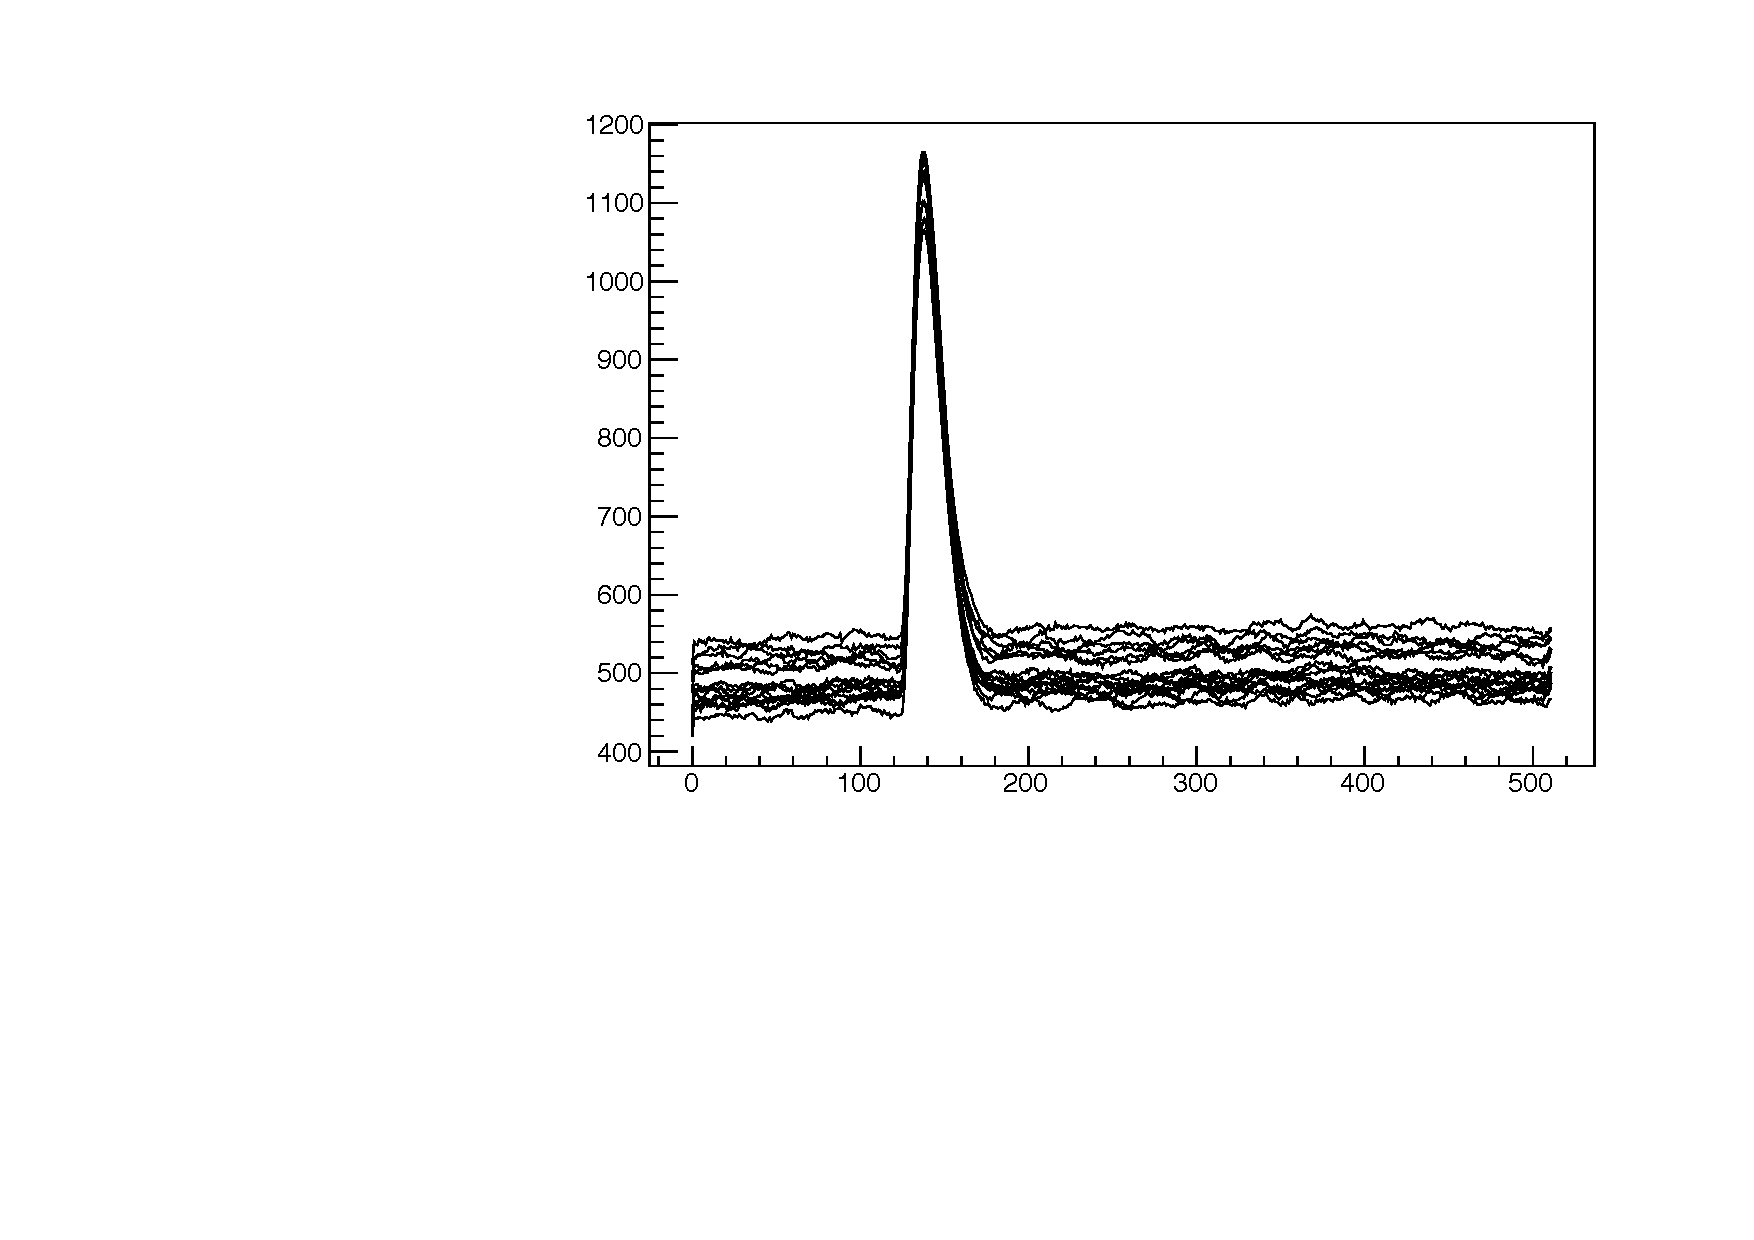
\includegraphics[width=1.0\columnwidth]{figures/waveformRaw}
	\caption{(Top) Example waveforms of the four FPN channels. (Bottom) Raw Waveforms without any FPN or background subtraction.}
	\label{fig:FPN_Raw}
\end{figure}

Further correction is achieved by subtracting the overall baseline, found by averaging the first and last 10 time buckets, from the FPN corrected signal. Examples of the waveforms corrected by the FPN and baseline subtraction are shown in Fig. \ref{fig:Waveform_Corrected}.

\begin{figure}[hbt]!
    \centering
    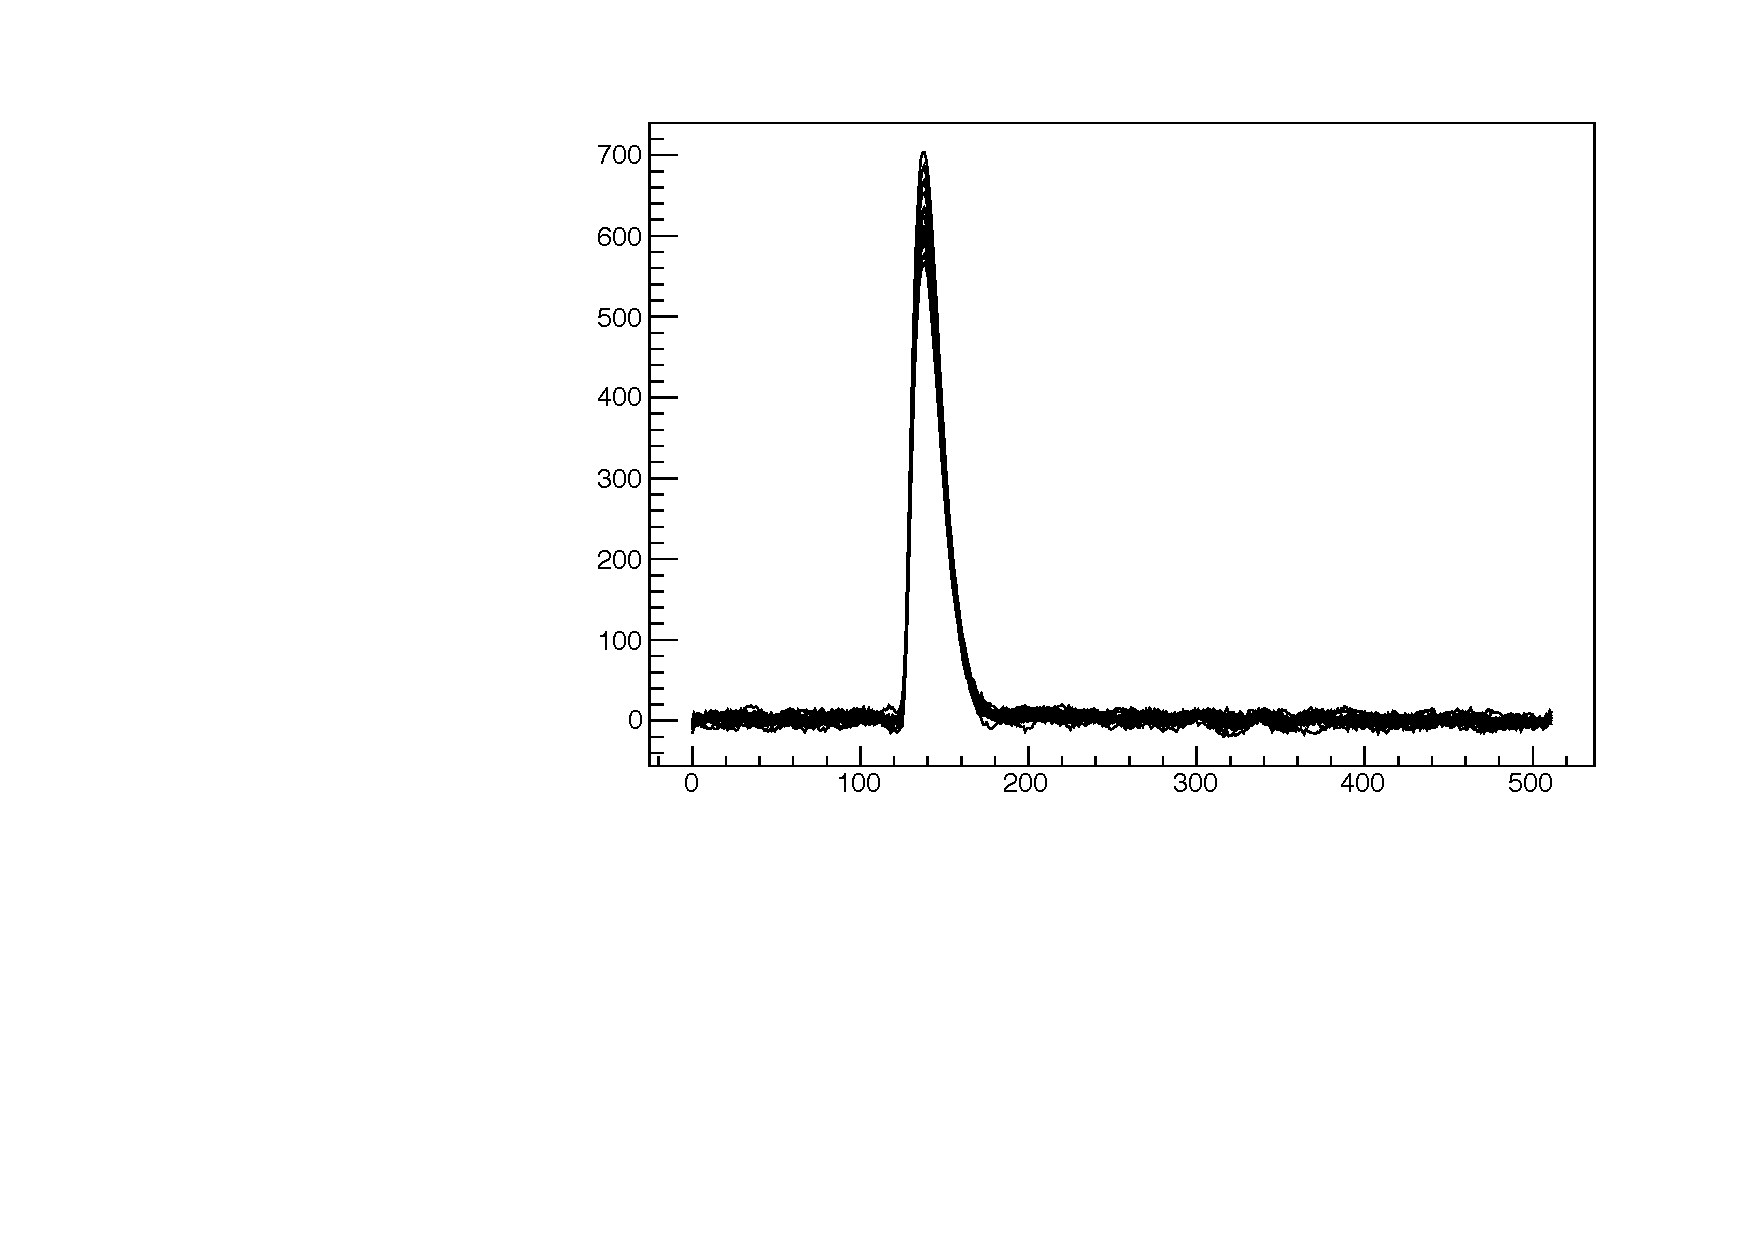
\includegraphics[width=1.0\columnwidth]{figures/waveformCorrected}
    \caption{Waveforms corrected with FPN and background subtraction.}
    \label{fig:Waveform_Corrected}
\end{figure}

\subsection{Chain and Strip Matching \label{CSmatching}}

To perform track reconstruction in the side regions of the Micromegas detector, chains and strips must be matched with each other since chains run parallel to the beam axis along the entire Micromegas while the strips run perpendicular to the beam axis along the entire side region. Chains and strips were matched using the time recorded for each channel. When the charged particle travels over the side region, any chains and strips that correspond to the proton track position should have the same drift time. If the track is not parallel to the microMegas plane, the matched chains and strips based on the same time should form a well defined track. An example of such event is shown in Figure \ref{fig:ChainStripExample}. When the track is parallel to the microMegas detector, the timing for the chains and strips will be the same and instead of a defined track like that in Figure \ref{fig:ChainStripExample}, it forms a square of matched chains and strips. For cases like this, the first point in the matched square closest to the origin and the point furthest away from the origin are chosen to form the track.

\begin{figure}[hbt!]
	\centering
    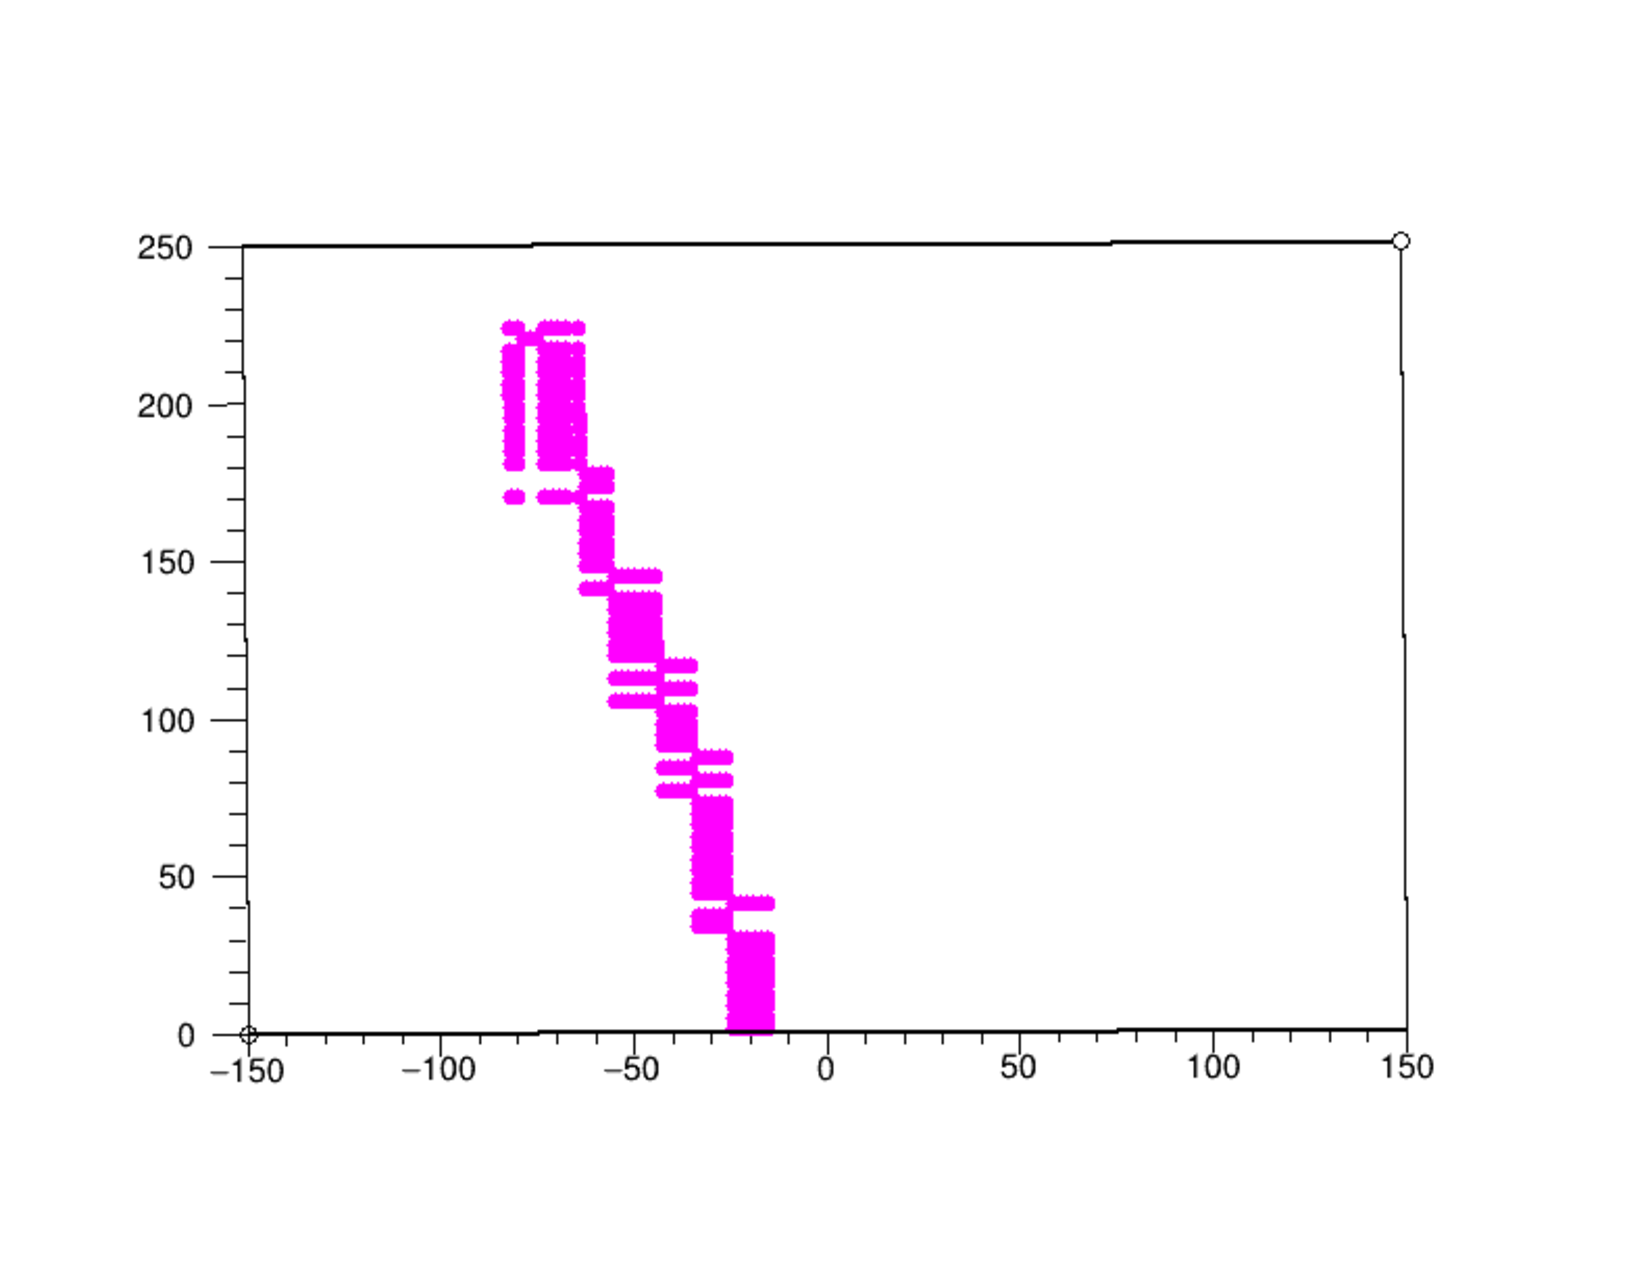
\includegraphics[width=0.5\textwidth]{figures/TexAT_Example_Track}
    \caption{An example of matched chains and strips for a single event that can then be used to reconstruct a track.}
    \label{fig:ChainStripExample}
\end{figure}

\subsection{Track Reconstruction - Hough Transform}

Signal in the TPCs is often contaminated by ``noise'' - random pads firing in coincidence with the  track but seemingly unrelated to it. We have used the two dimensional Hough transform to reduce influence of this ``noise'' on the track reconstruction.

The Hough transform is a feature extraction technique that has been very successful in image analysis and image processing \cite{Duda:1972}. The Hough transform was originally used to identify lines in an image and in this analysis, to find tracks (lines) through data points. This method works by transforming points into a parameter space and a voting procedure is used to find peaks in this parameter space. For each point $(x, y)$ the Hesse normal form is calculated

\begin{equation}
	d = x \cos \theta + y \sin \theta,
	\label{eq:Hesse}
\end{equation}

where $d$ is the distance of closest approach to the origin and $\theta$ is the angle between the x-axis and the line connecting the origin to the closest point as shown in Figure \ref{fig:HoughDiagram}. The $(d, \theta)$ parameter space is called the Hough space. For every point in the data, $\theta$ is varied from $0$ to $\pi$ and $d$ is calculated.

\begin{figure}[hbt!]
	\centering
    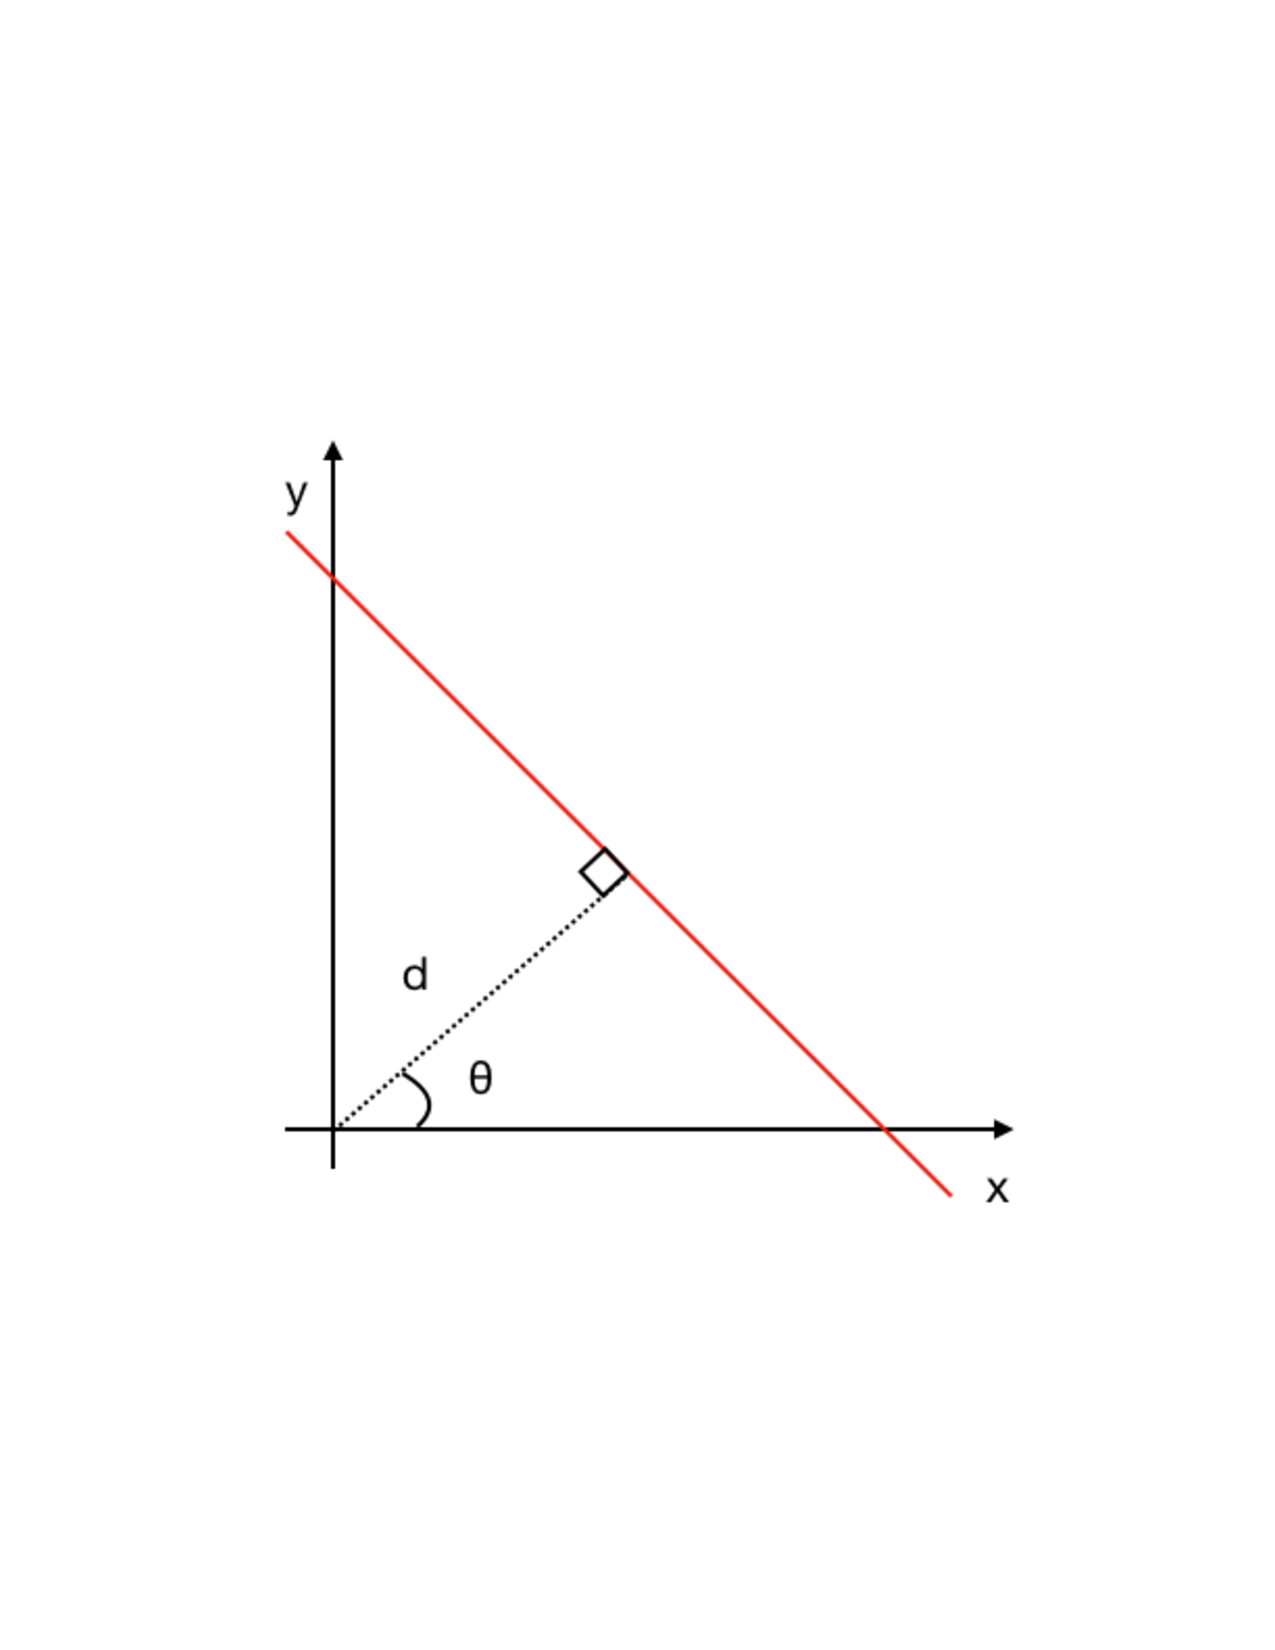
\includegraphics[width=0.5\textwidth]{figures/HoughTransform}
    \caption{Diagram of the $d, \theta$ parameters in two dimensions.}
    \label{fig:HoughDiagram}
\end{figure}

The algorithm used to find the optimal $(d, \theta)$ was to search through all angles and find the lowest standard deviation in $d$. A simple example with noise is shown in Figure \ref{fig:HoughExample}. In the top of Figure \ref{fig:HoughExample}, there is a straight line formed by the blue colored points while the orange colored points are noise. The Hough space is shown at the bottom of Figure \ref{fig:HoughExample} illustrating the point where the standard deviation is minimal. By finding the optimal parameters $(d, \theta)$, we find the best fit of the data that is not affected by noise.

\begin{figure}[hbt!]
	\centering
	\begin{subfigure}{.5\textwidth}
  		\centering
  		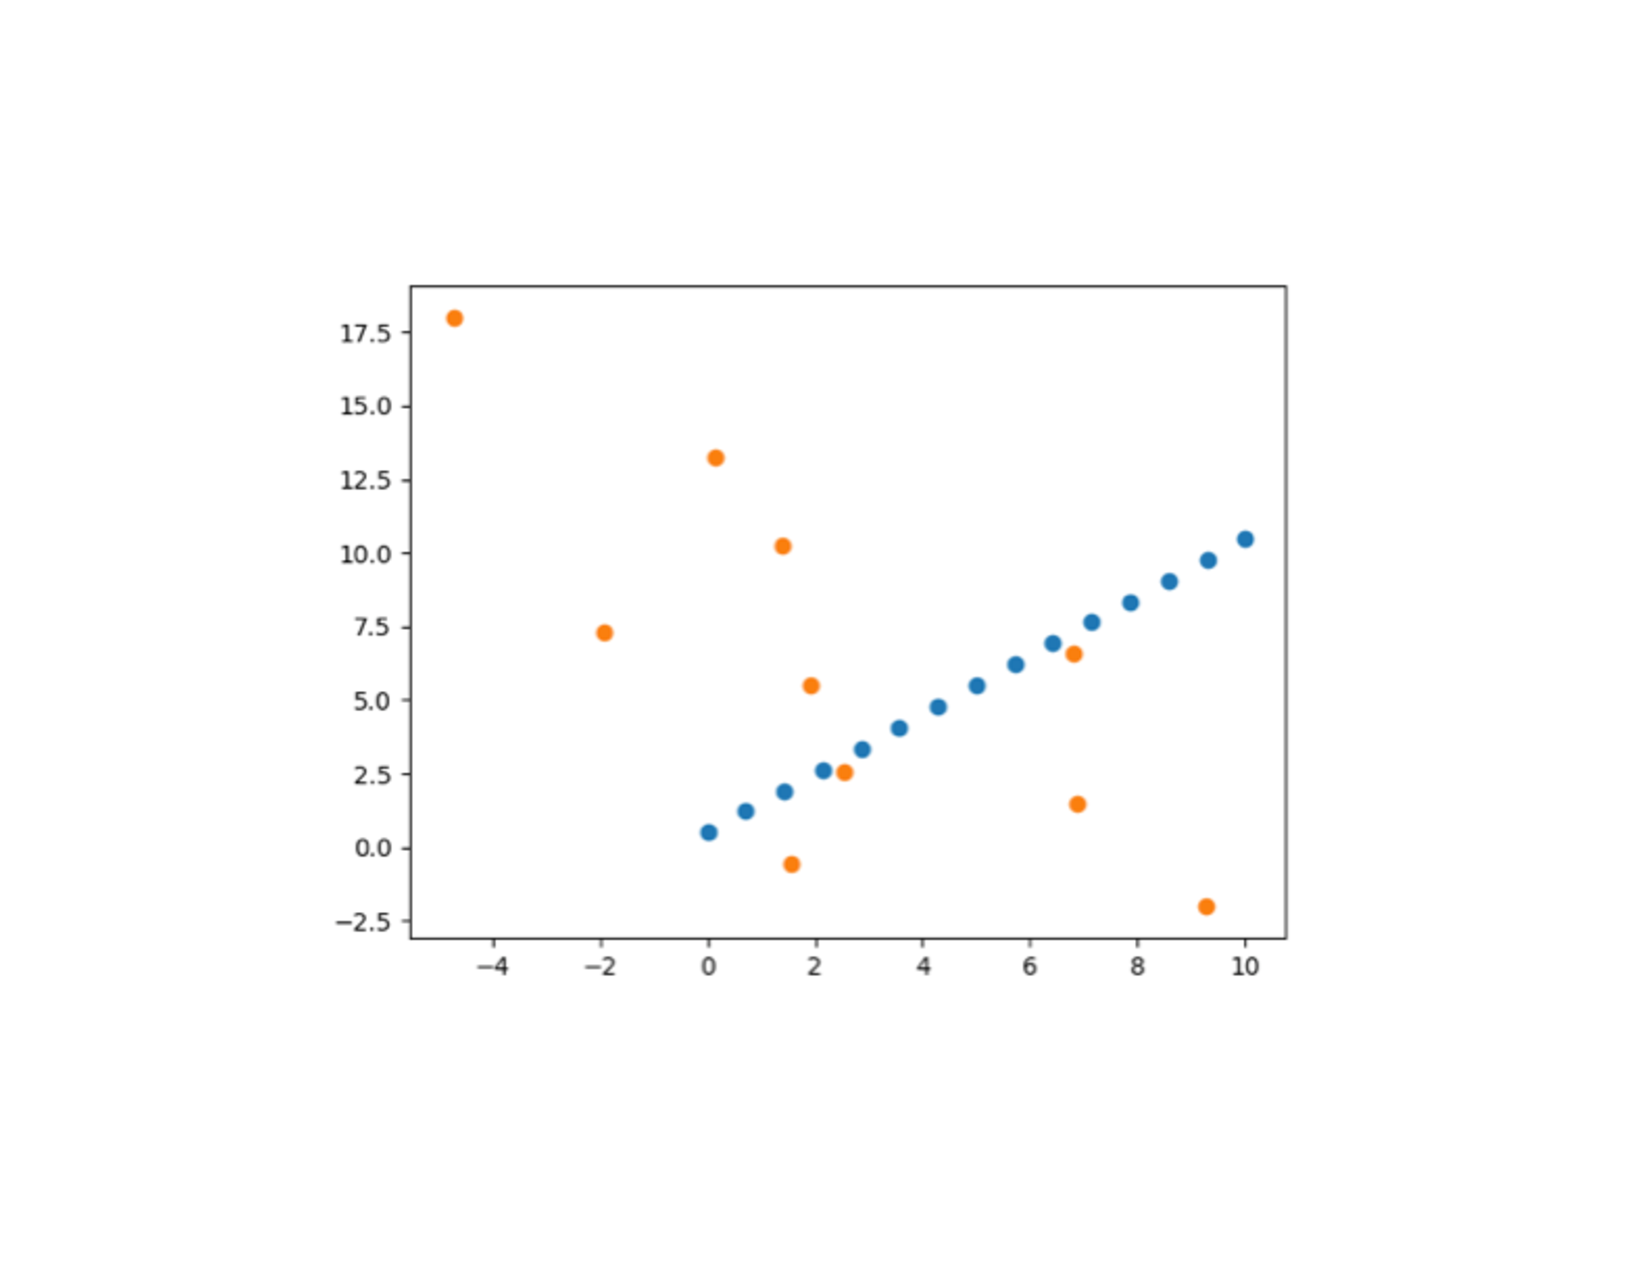
\includegraphics[width=\linewidth]{figures/HoughExample1}
	\end{subfigure}%
	\\
	\begin{subfigure}{.5\textwidth}
  		\centering
  		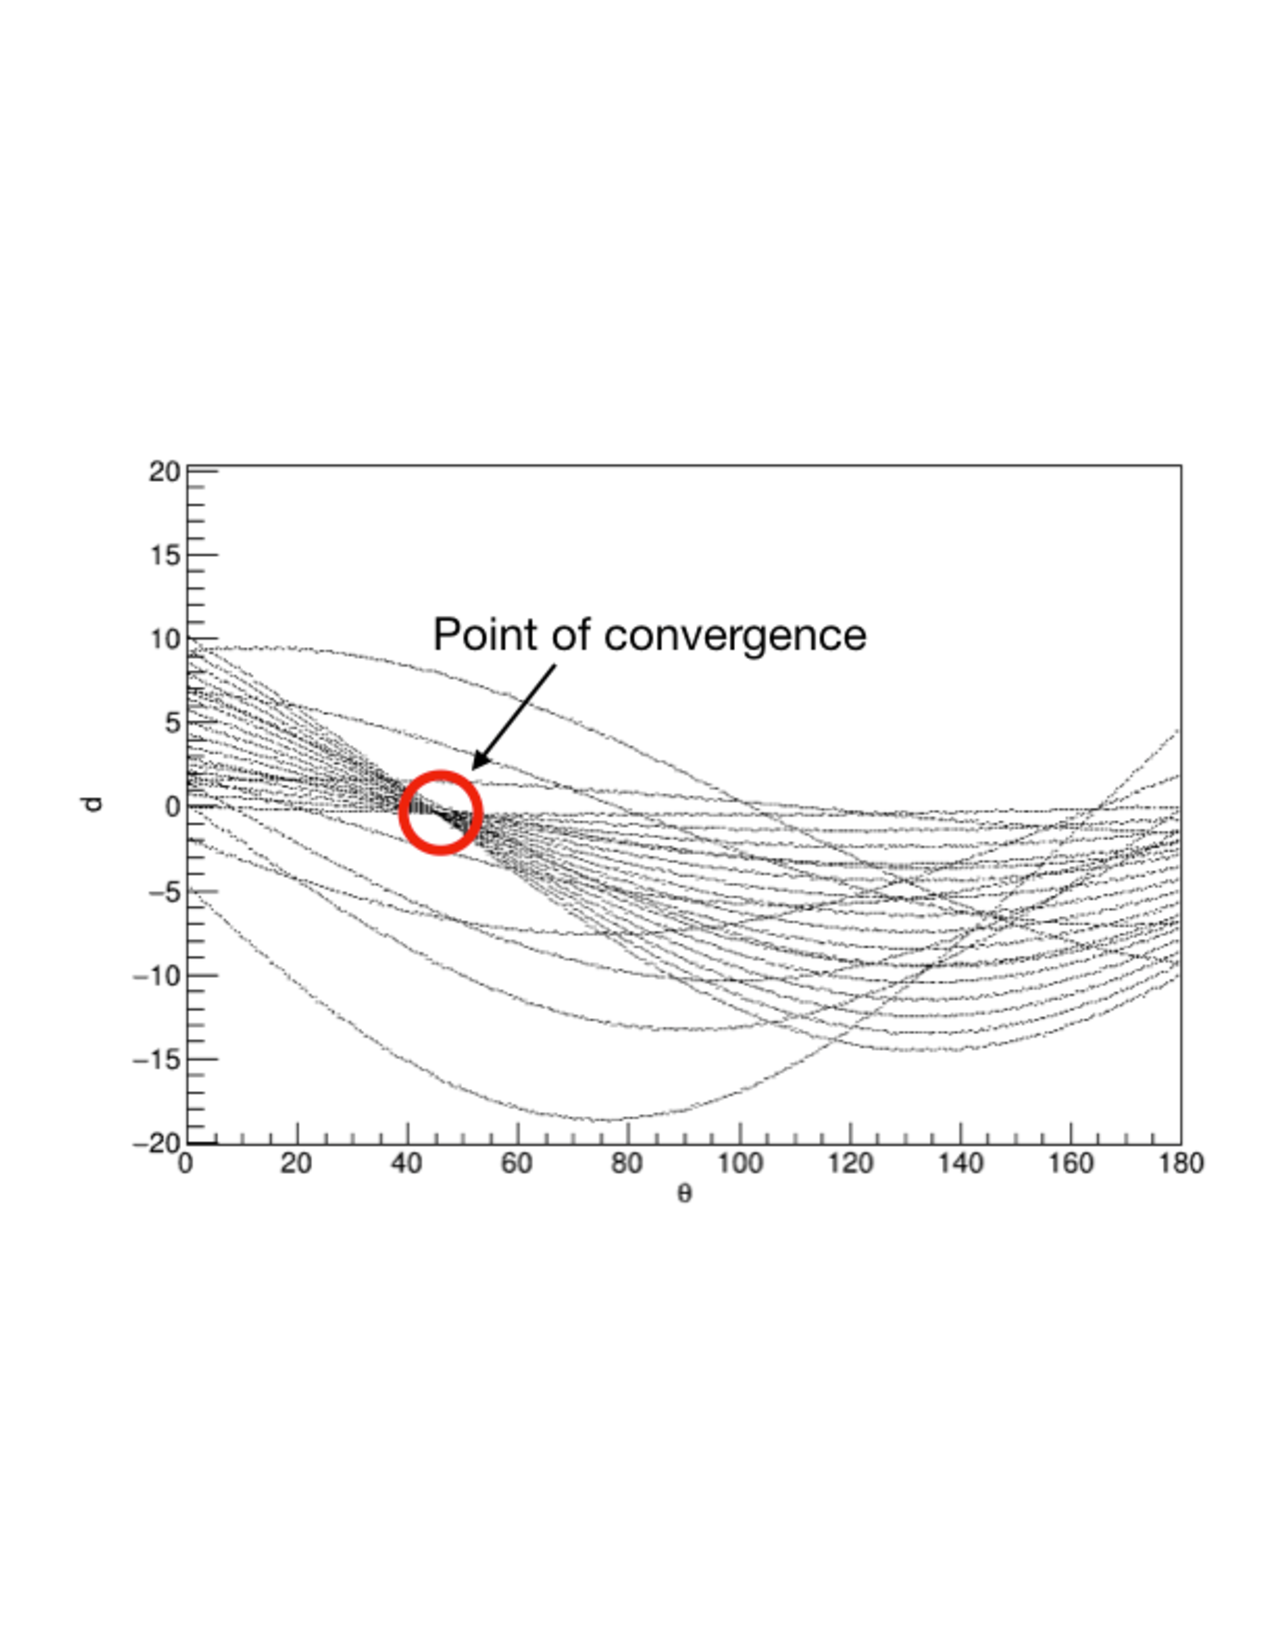
\includegraphics[width=\linewidth]{figures/HoughExample2}
	\end{subfigure}
	\caption{(Top) A straight line (blue points) with scattering noise (orange). (Bottom) The Hough space of the top points. Outlined in the red is the minimal standard deviation of $d$ corresponding to the straight line of blue points.}
	\label{fig:HoughExample}
\end{figure}

 \subsection{Alpha Source Test in Gas}
 
We have tested the chains and strips matching technique and a technique to fit tracks with noise using the Hough transform using an $\alpha$ source in gas. The gas chosen for this measurement was methane at $50$ Torr so that the 5 MeV $\alpha$ particles propagate through the entire active volume of the scattering chamber and make it to the Si detector while also depositing enough energy in the gas to make tracks. The $\alpha$ source was placed approximately 60 mm behind the Micromegas plate facing the Si detectors. An accumulation of the tracks in the XY-plane are shown in Fig. \ref{fig:TexATAlphaTracksXY}. Zero on the y-axis in Figure \ref{fig:TexATAlphaTracksXY} corresponds to the start of the Micromegas plate and shown are all the tracks that end up in the forward and side wall Si detectors. The tracks are converging at the (0 mm,-60 mm) point that has about the size of the source ($\sim 5 mm$ along the x-axis).
 
\begin{figure}[hbt!]
	\centering
	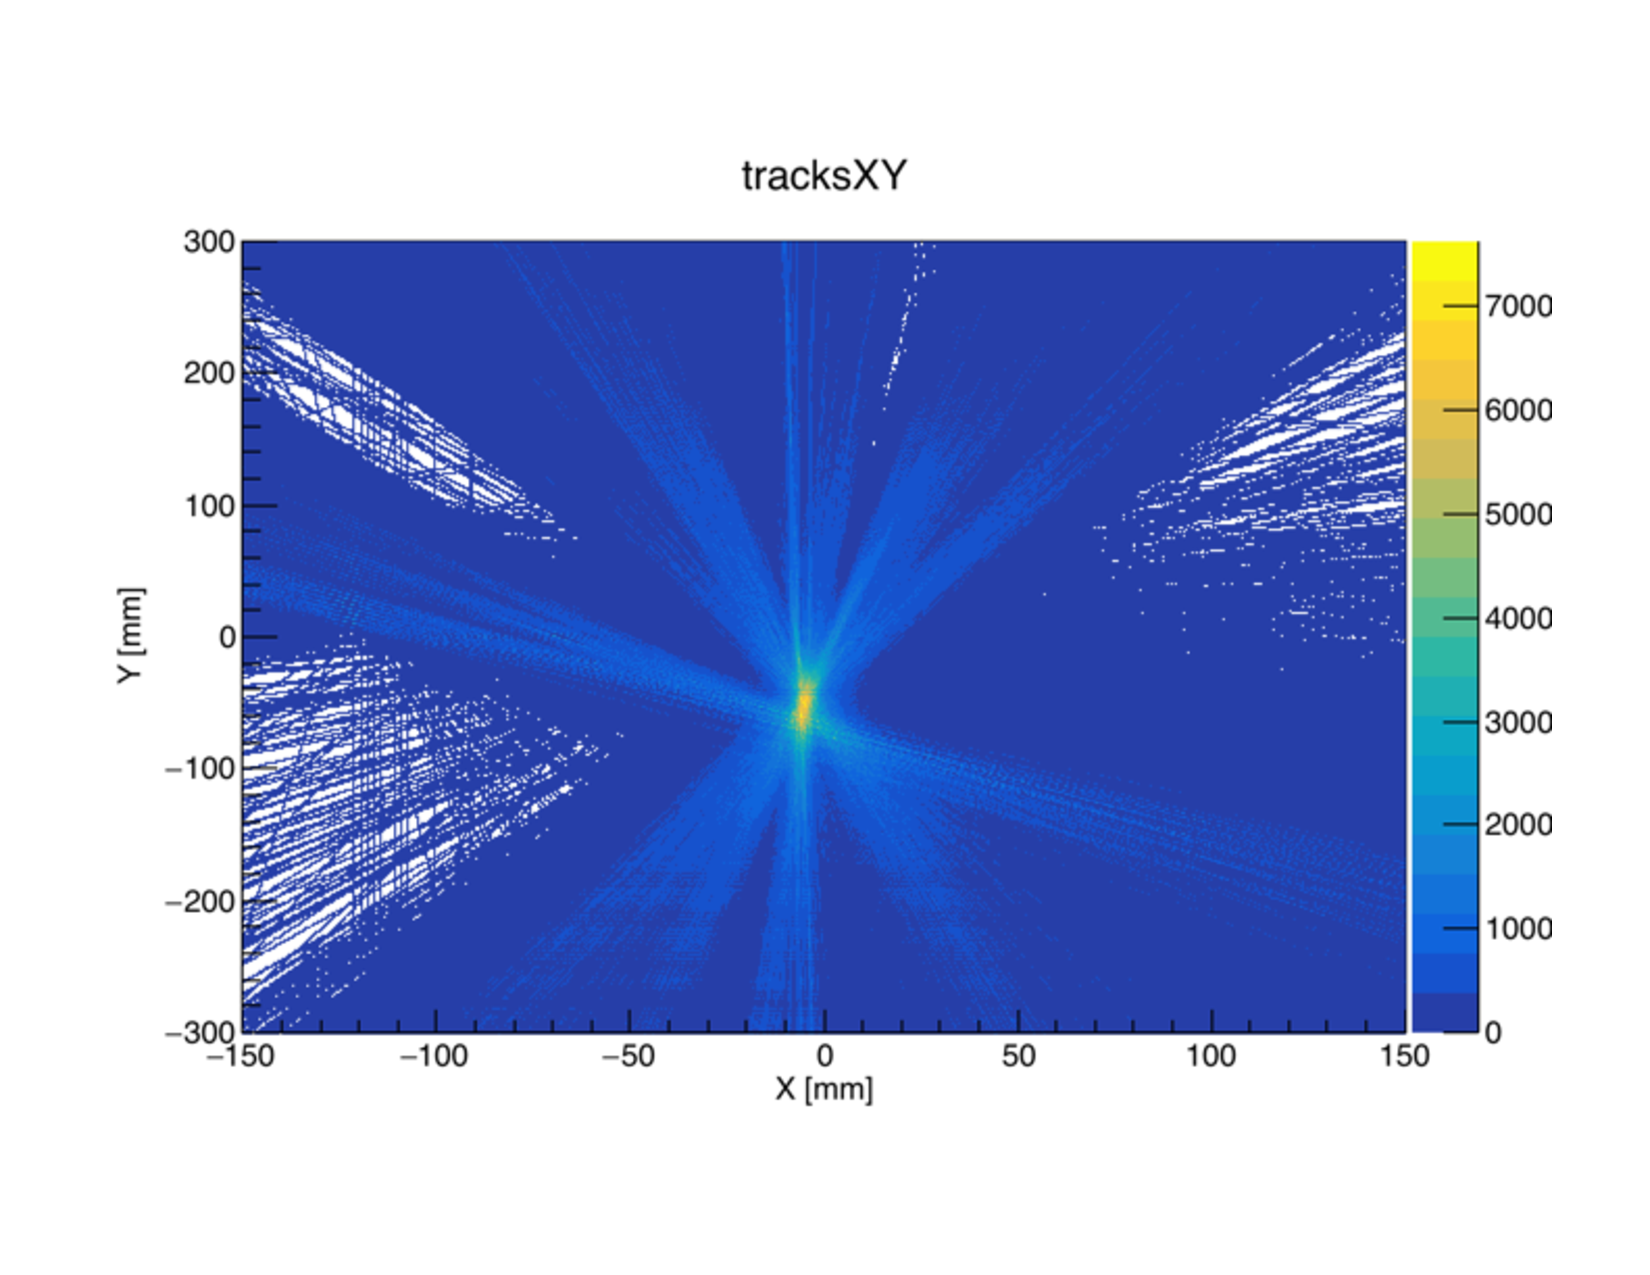
\includegraphics[width=0.5\textwidth]{figures/TexATAlphaSourceTrackingXY}
    \caption{An accumulation of the alpha source tracks in the XY-plan in the forward and side walls. 0 mm on y-axis corresponds to the beginning of the Micromegas plate. All of the tracks converge to $\sim -60$ mm where the source was located.}
    \label{fig:TexATAlphaTracksXY}
\end{figure}

Beyond plotting the XY-plane of all the tracks, we also judge how well our track reconstruction is by plotting the projected end point of the track at the location of the Si detectors plane. When fitting the tracks, none of the Si information is used to constrain the track reconstruction. The XZ-plan reconstruction of track end point at the location of the Si detectors for the forward wall are shown in Figure \ref{fig:TexATTracksForwardSi}. We clearly see the definitions of all nine Si detectors on the forward wall and also the gap corresponding to the missing Si detector in the top left corner. Although no Si information is used in the track reconstruction, it is recorded which Si quadrant fired. By using this information, we can get a better idea to how well the track reconstruction is by only plotting the XZ projection if certain quadrants have fired. By plotting the reconstructed track endpoints only for opposite corners of the Si detectors a checker-board pattern is achieved, just as expected \ref{fig:TexATTracksForwardSi_Corners}. Very good position reconstruction for each of the quadrants is evident.

\begin{figure}[hbt!]
	\centering
	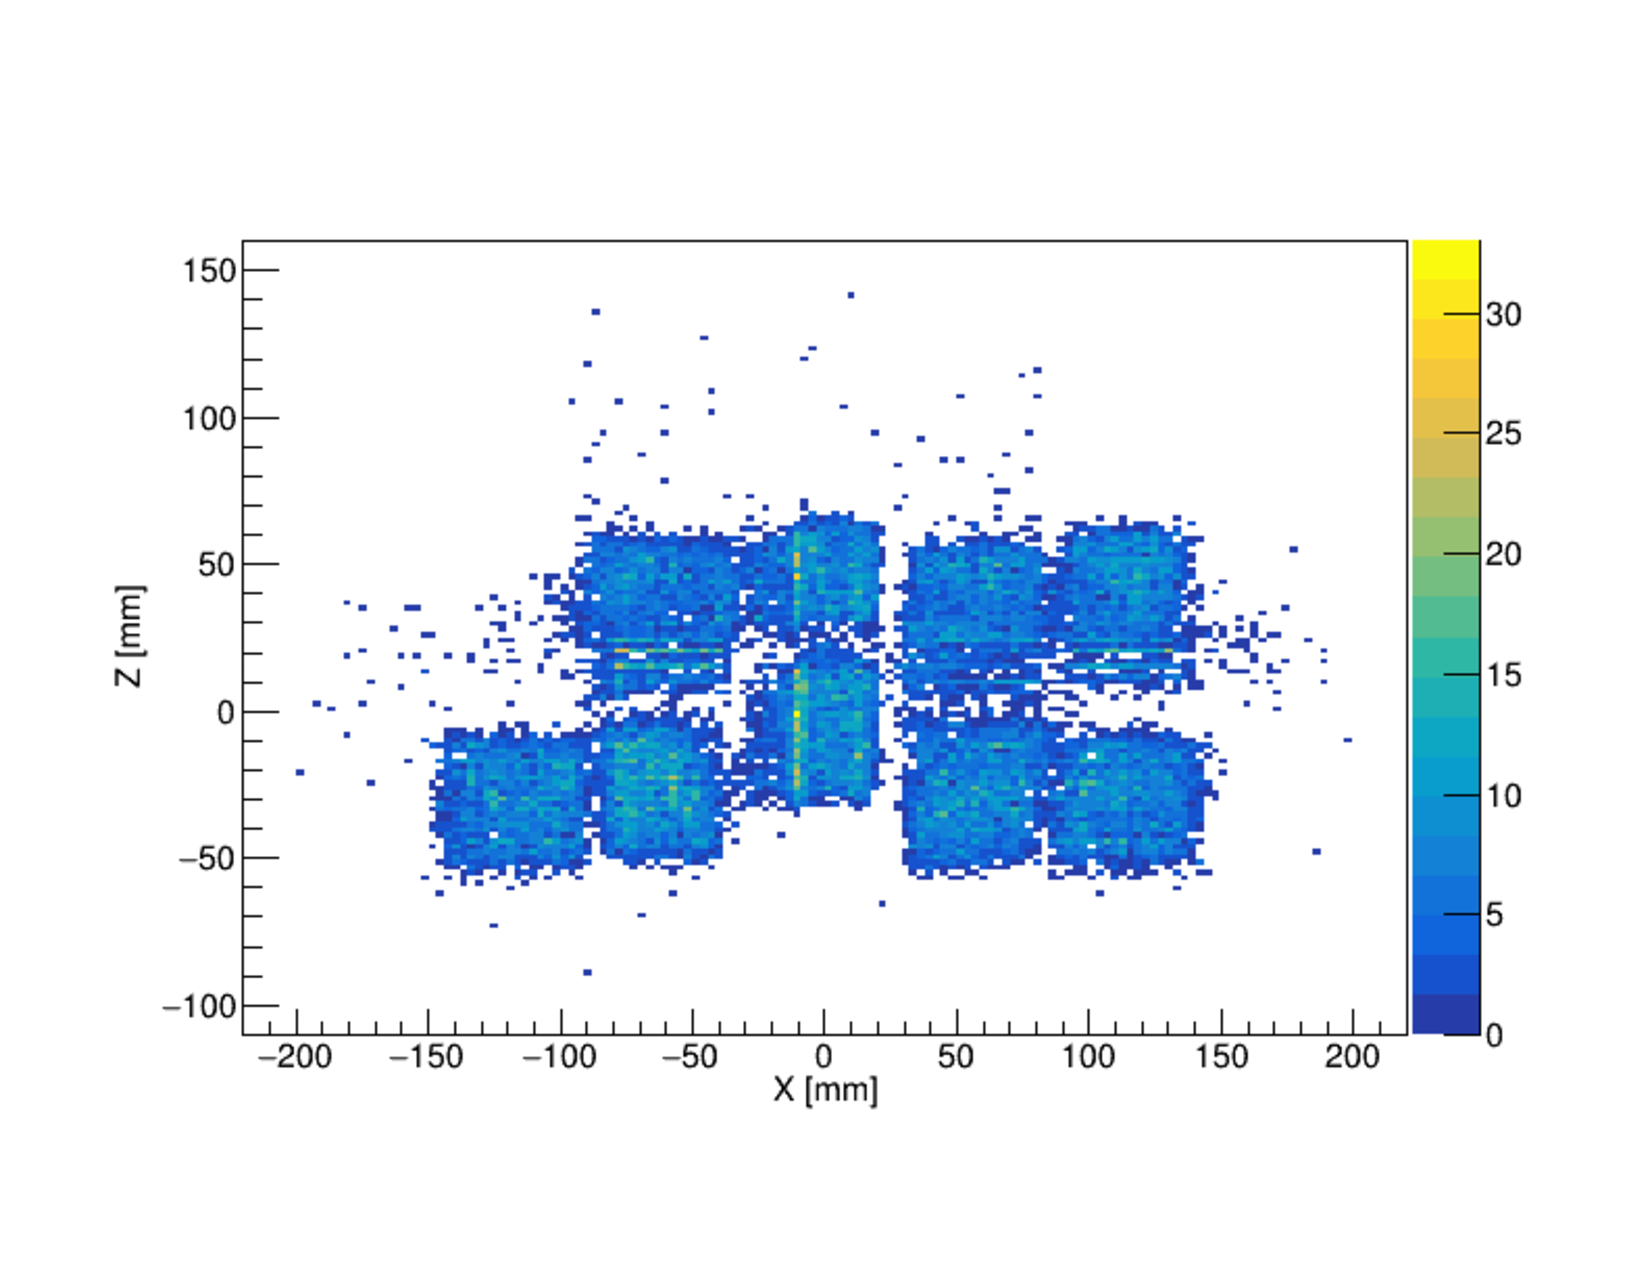
\includegraphics[width=0.5\textwidth]{figures/TexATTracksForwardSi}
    \caption{The XZ projection of the forward Si wall.}
    \label{fig:TexATTracksForwardSi}
\end{figure}

\begin{figure}[hbt!]
	\centering
	\begin{subfigure}{.5\textwidth}
  		\centering
  		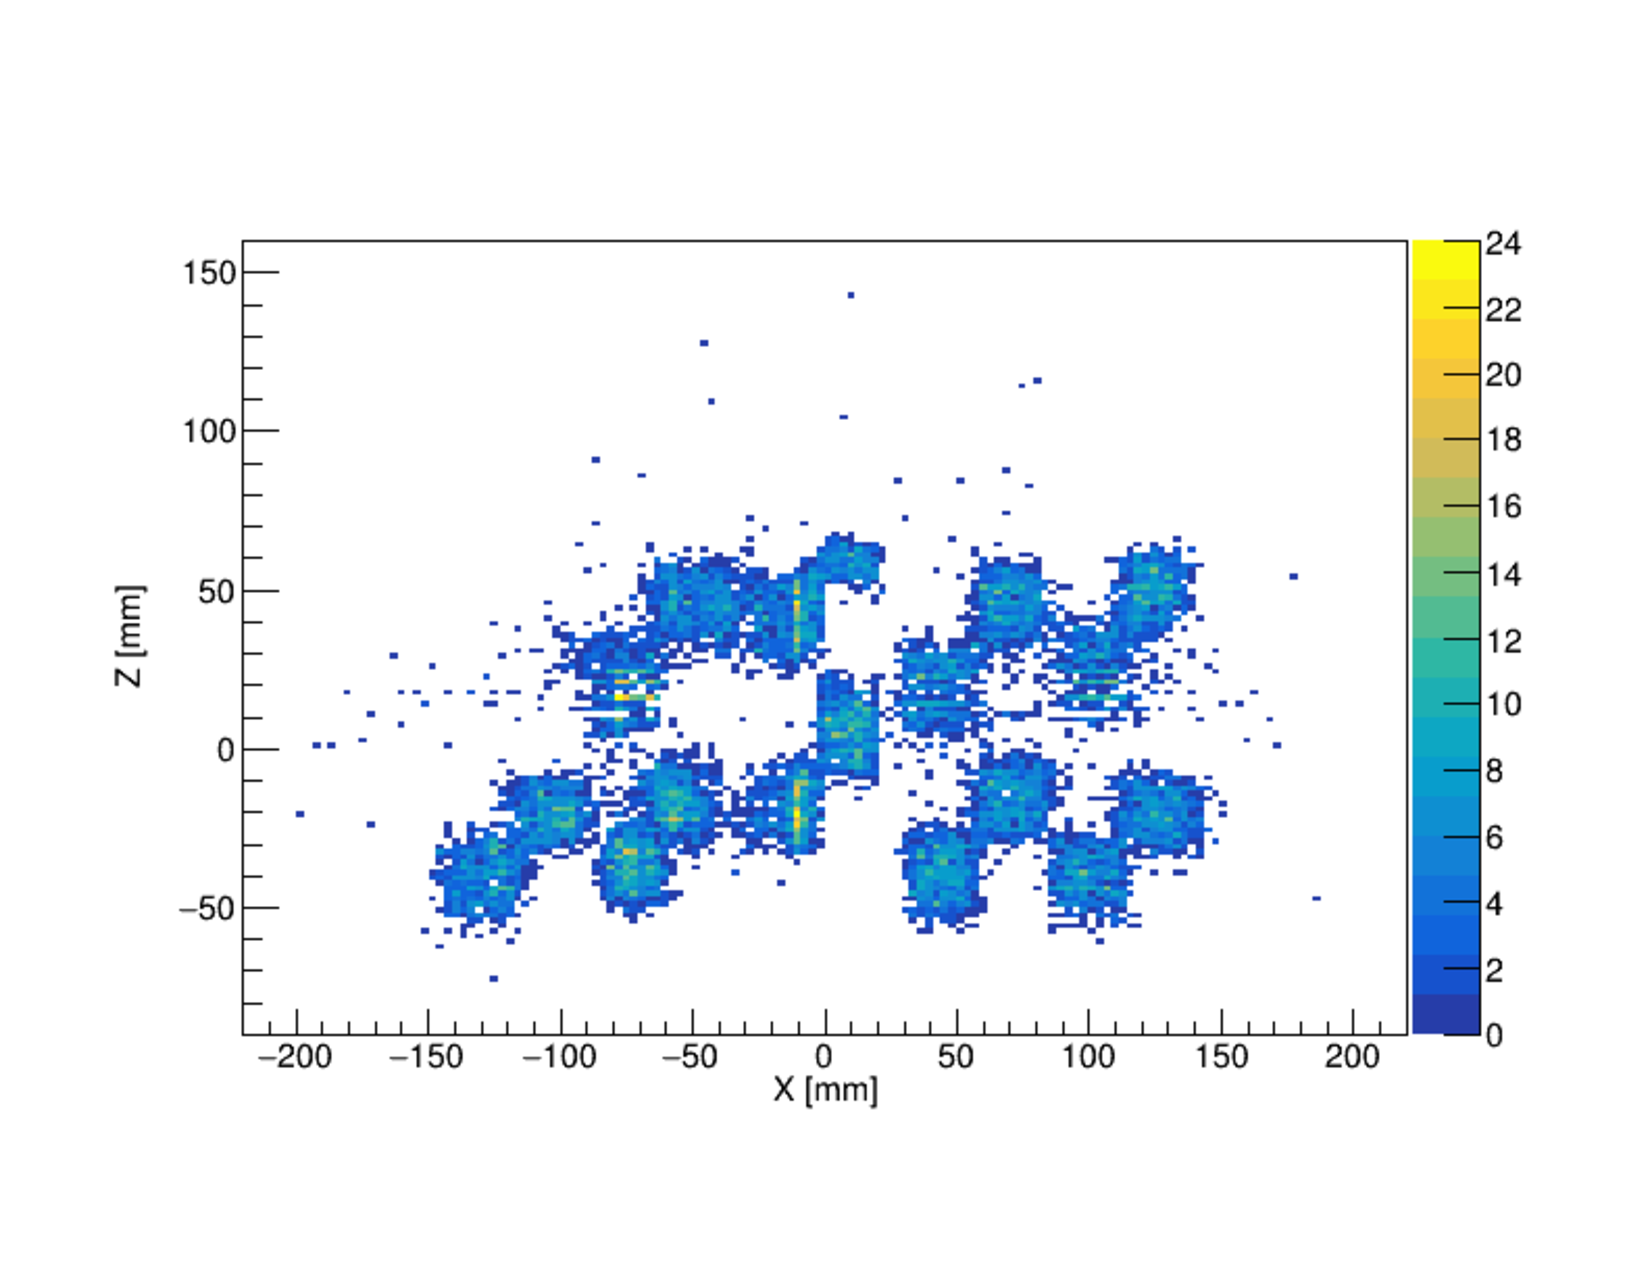
\includegraphics[width=\linewidth]{figures/TexATTracksForwardSi_corners1}
	\end{subfigure}%
	\\
	\begin{subfigure}{.5\textwidth}
  		\centering
  		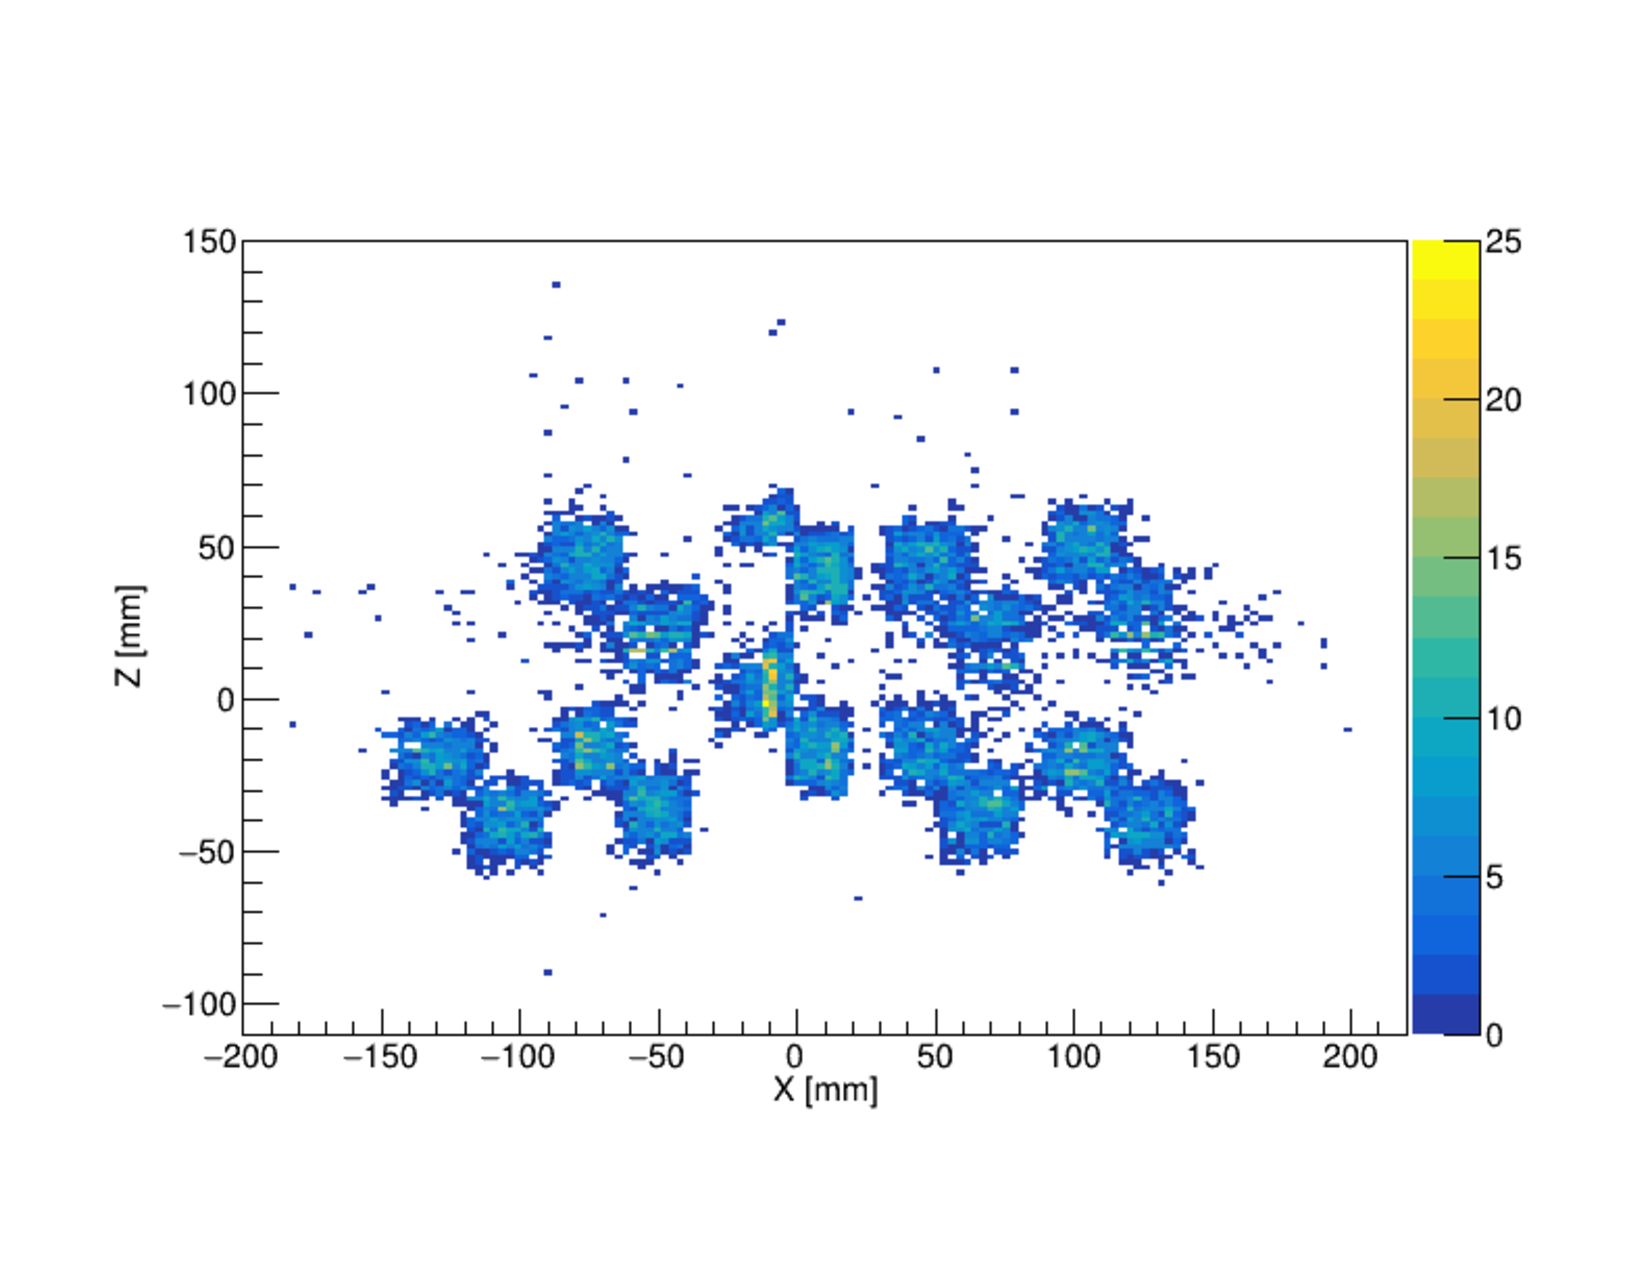
\includegraphics[width=\linewidth]{figures/TexATTracksForwardSi_corners2}
	\end{subfigure}
	\caption{(Top) XZ projection of the Si wall choosing the lower left and upper right quadrants of each Si detector. (Bottom) XZ projection of the Si wall choosing the upper left and lower right quadrants of each Si detector.}
	\label{fig:TexATTracksForwardSi_Corners}
\end{figure}

\section{Commissioning experiments}%Marina's edition

To date we have conducted four types of experiments with TexAT:

\begin{itemize}
	\item Resonance elastic scattering of protons with stable and rare isotope beams - $^{12}$C+p and $^8$B+p
	\item Resonance elastic scattering of $\alpha$-particles with rare isotope beams - $^{10}$C+$\alpha$ and $^{14}$O+$\alpha$
	\item Direct measurements of fusion reaction cross section - $^8$B+$^{40}$Ar
	\item $\beta$-delayed charged particle emission - $^{12}$N $\beta$ decay to $^{12}$C Hoyle state with subsequent emission of three $\alpha$-particles.
\end{itemize}

In this paper we will only focus on describing the experimental procedures for the proton elastic scattering measurements, the experiments that were used as commissioning runs for TexAT and are at the most advanced stages of analysis at this time. 


For these experiments, stable beams of $^{12}$C and $^6$Li were delivered by the K150 cyclotron accelerator at the Texas A\&M University Cyclotron Institute. The $^8$B beam was produced using Magnetic Achromat Recoil Separator (MARS) \cite{MARS} with the reaction $^6$Li($^3$He,n)$^8$B. The energy of the $^8$B beam was 60 MeV and the intensity was about 1,000 pps.
In addition to the regular TexAT detector components/arrays, we have installed a thin scintillator, read out by two PMTs, upstream from the TexAT chamber. This detector was used during the run with $^8$B beam to count the beam particles before the TexAT setup and help removing the beam contaminants. The scintillator was removed for the run with $^{12}$C (the intensity was about 10$^5$ pps). The PMT signals from the sides of the scintillator were fed to a CFDs with a threshold high enough to trigger only on the $^{8}$B beam particles leaving the beam contaminants, primarly  $^3$He, below the threshold. The two outputs from the CFD were sent to a logic unit that triggered when both PMT signals were above the threshold. The trigger was then sent to a CAEN VME Scalar unit to count the number of beam ions for overall normalization. The CAEN Scalar was placed on its own data acquisition system separate from the GET electronics. A windowless Ionization chamber (IC) was also placed inside the TexAT chamber, just after the entrance window to count and identify the beam particles. To trigger the GET electronics we required a coincidence between the external signal from the IC and at least one Si detector channel (this is the so-called L0L1 mode in GET electronics). This was important to avoid triggering on events associated with $^3$He ions in the beam. Unlike $^8$B,  these light ions do not stop in the gas and trigger the Si detector located on the beam axis, however they do not leave enough energy to trigger the IC, therefore they are vetoed.  The digitizer was set to 25 MHz meaning that the waveforms were recorded every 40 ns and the total timeframe window was 20.48 $\mu$s (512$\times$40 ns). The system was set to zero suppression mode so that only the channels that fired above the threshold were recorded and written to disk, all the other channels were ignored.

%Marina end

%In addition to the regular TexAT detector components/arrays we have installed a scintillator, read out by two PMTs, upstream from the TexAT chamber. These were not used during the run with the stable beam of $^{12}$C (intensity was about 10$^5$ pps), but were useful for the run with $^8$B beam. The %$^8$B beam was produced using Magnetic Achromat Recoil Separator (MARS) \cite{MARS} in reaction $^6$Li($^3$He,n)$^8$B. The energy of the $^8$B beam was 60 MeV and intensity was about 1,000 pps. The stable beams of $^{12}$C and $^6$Li were delivered by the K150 cyclotron accelerator at the Texas A\&M University Cyclotron Institute.
%The PMT signals were fed to a CFDs with a threshold high enough to only trigger on the $^{8}$B beam particles with all other beam contaminants below the threshold (primarily $^3$He). The two outputs from the CFD were sent to a logic unit that triggered when both PMTs fire above the threshold. The trigger was then sent to a CAEN VME Scalar unit to count the number of beam ions for overall normalization. The CAEN Scalar was placed on its own data acquisition system separate from the GET electronics. To trigger the GET electronics we have required coincidence between the external signal from ionization chamber and at least one Si detector channel (this is the so-called L0L1 mode in GET electronics). This was important to avoid triggering on events associated with direct $^3$He coming with the beam. These light ions do not stop in the gas (unlike $^8$B) and trigger the Si detector located on the beam axis, but they do not leave enough energy to trigger the ionization chamber - therefore they are vetoed. The digitizer was set to 25 MHz meaning that the waveforms were recorded every 40 ns and the total timeframe window was 20.48 $\mu$s (512$\times$40 ns). The system was set to zero suppression mode so that all channels that fired above the threshold are recorded and written to disk but all other channels that have no hits or have hits below the threshold are ignored.

\subsection{Beam Particle Identification}

In the experiment with the stable beam ($^{12}$C) there were no beam contaminants. In the rare isotope beam experiment the separation of the $^{8}$B ions from the small contamination, mostly of $^3$He was done using the energy and timing from the ionization chamber. By measuring the energy deposited in the IC and the time relative to the signal in the Si detector, it was possible to cut out the small amount of contamination. Note that the CH$_4$ gas pressure was set to (435 Torr) so that $^8$B ions were stopped long before they could hit the Si detector at zero degrees. Therefore, the correlation between the time of a hit in a Si detector and that of a  $^8$B ion in the ionization chamber is a signature that a nuclear reaction with $^8$B produced a light recoil. Fig. \ref{fig:9CIonization} shows the energy deposited in the IC and the time relative to the Si detector (comment: it would be better to have a 2D plot with Energy and time to show the correlation). For all ``good'' events, the ionization chamber time is mostly determined by the shaping time delay between the ionization chamber signal and that of the Si-detectors. We have used the internal GET preamps for the Si, and an external MESYTEC shaper for the ionization chamber signal that was than fed into the GET electronics, bypassing the internal preamp and internal shaper. The energy and timing peaks of the $^{8}$B beam in the ionization chamber is clearly seen in Fig. \ref{fig:9CIonization} . These two quantities were used to make a cut on the events related to $^{8}$B beam.






%For the experiment with stable beam ($^{12}$C) no contaminants were coming with the beam. For the rare isotope beam experiment separating the $^{8}$B beam ions from the small contamination of mostly $^3$He was done using the energy and timing from the ionization chamber. By measuring the energy deposited and the time relative to a signal in the Si detector, we can cut out the small amount of contamination. Note that the gas pressure was set so that $^8$B ions were stopped long before they could hit the Si detector at zero degrees. Therefore, correlation between timing of the hit in a Si detector and that of $^8$B ion in the ionization chamber is a signature of a nuclear reaction with $^8$B that produced a light recoil. Fig. \ref{fig:9CIonization} shows the energy and timing (with respect to the Si detector) of the ionization chamber. For all ``good'' events, the ionization chamber time should occur at around the same time determined by the shaping time delay between the ionization chamber signal and that of the Si-detectors. We have used internal GET preamps for the Si, and external MESYTEC shaper for the ionization chamber signal that was than fed into the GET electronics, bypassing the internal preamp and internal shaper. The energy and timing peaks of the $^{8}$B beam in the ionization chamber is clearly seen in Fig. \ref{fig:9CIonization} . These two quantities were used to make a cut on the events related to $^{8}$B beam.

\begin{figure}[hbt!]
	\centering
	\begin{subfigure}{.5\textwidth}
  		\centering
  		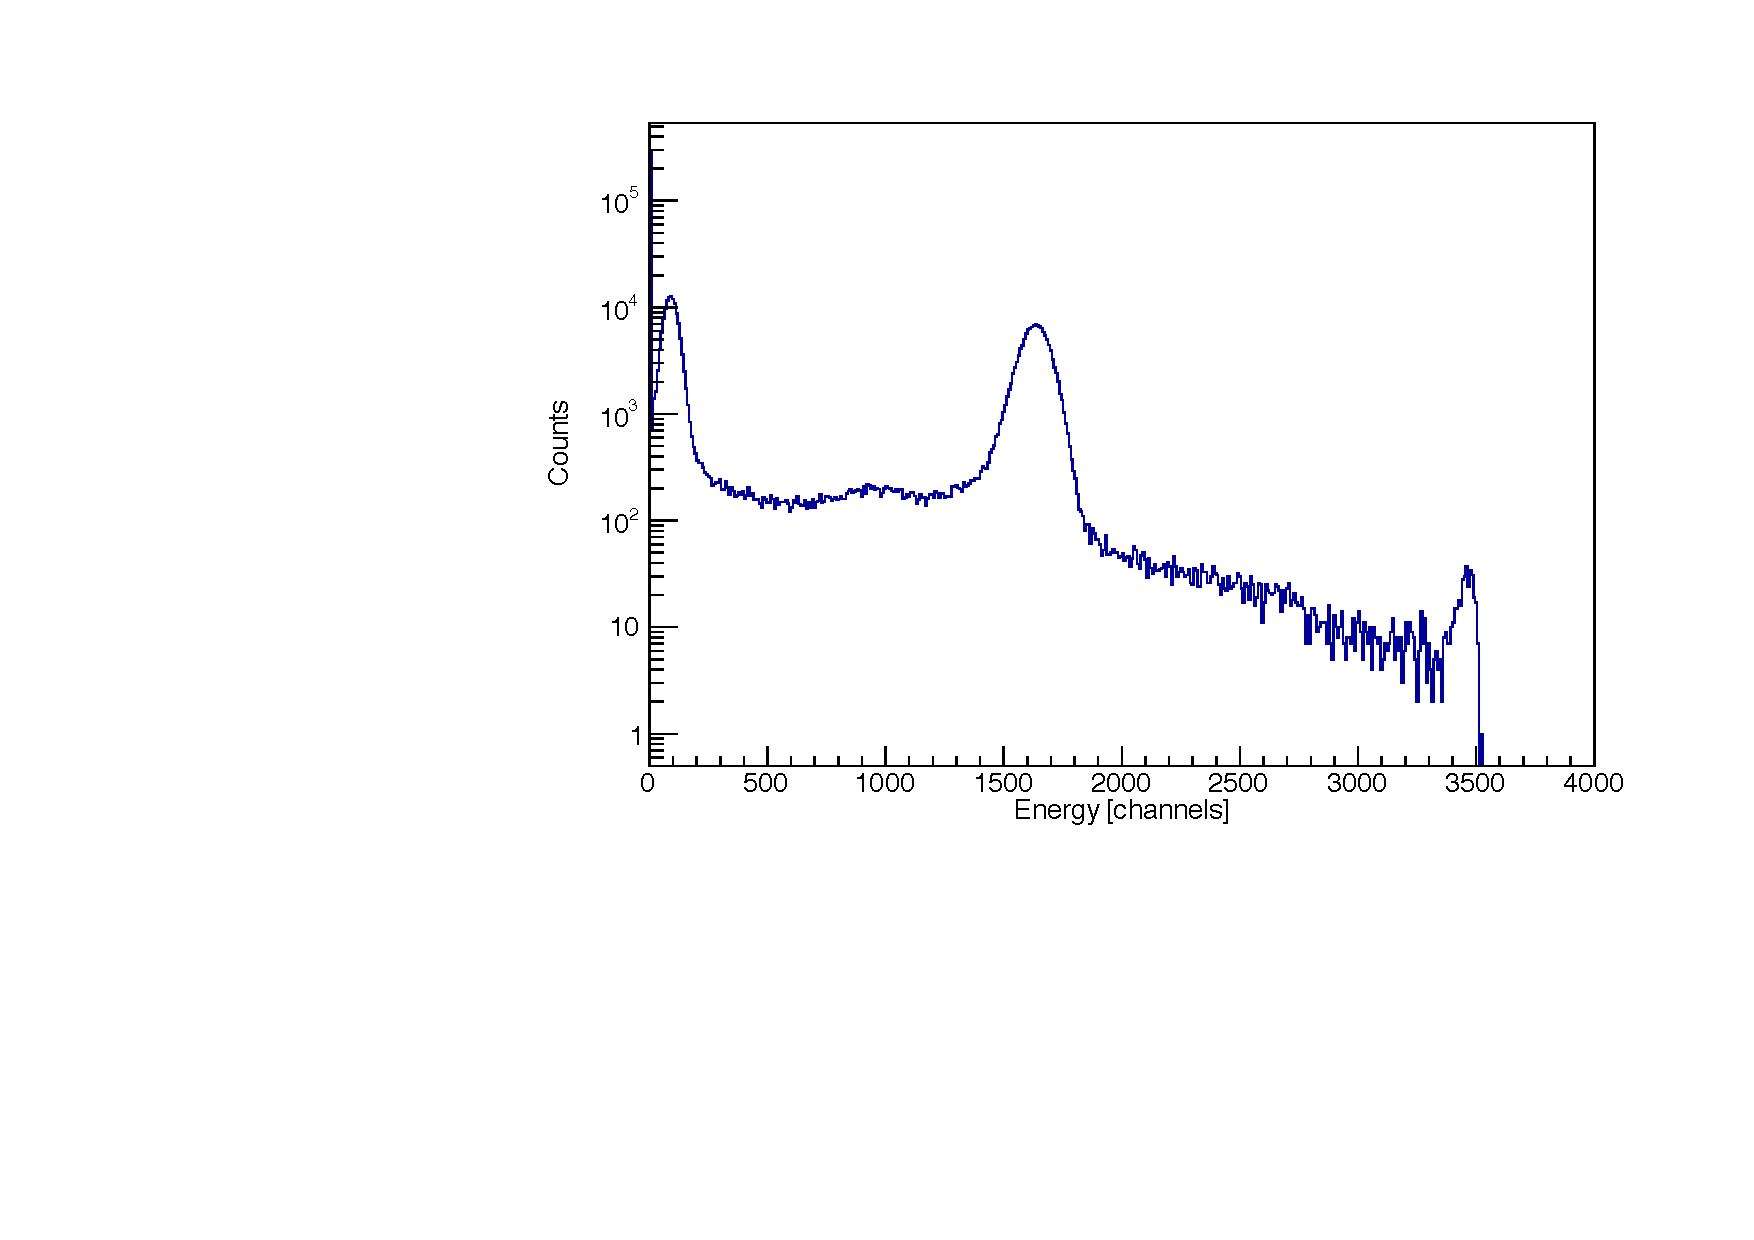
\includegraphics[width=\linewidth]{figures/9C_icE}
	\end{subfigure}%
	\\
	\begin{subfigure}{.5\textwidth}
  		\centering
  		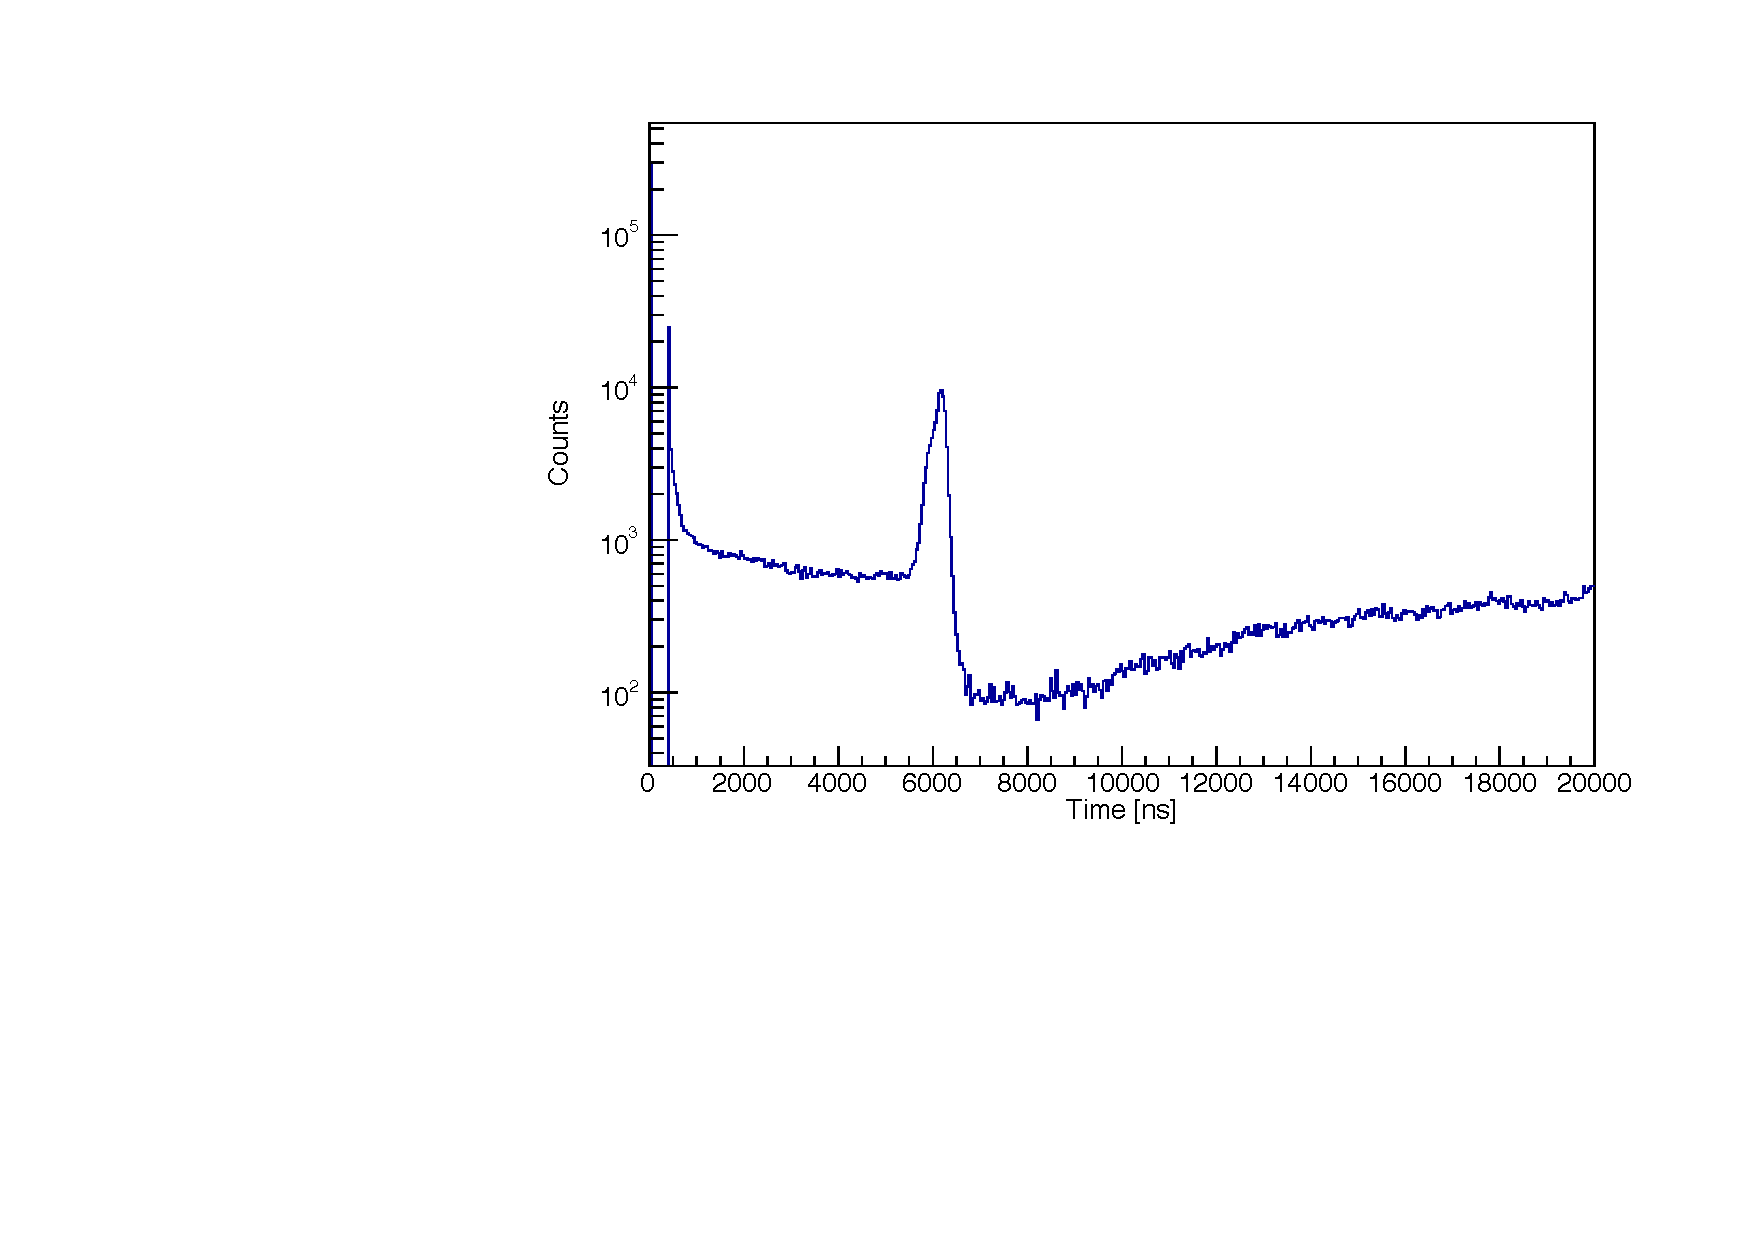
\includegraphics[width=\linewidth]{figures/9C_icT}
	\end{subfigure}
	\caption{(Top) The energy deposited in the ionization chamber. The $^{8}$B peak is located between channels 1300-1900. (Bottom) The time of the maximum of the ionization chamber. The beam particles corresponding to the Si hit fall between 5400 ns to 6500 ns.}
	\label{fig:9CIonization}
\end{figure}

\subsection{Tuning of the beam}

An important benefit of active target detector is the ability to measure the tracks of the incoming beam ions. This is especially useful when tuning the RIB into the chamber to make sure that it is coming in at the right angle and stopping in the correct location. Shown in Figure \ref{fig:9CBeamCumulative} is the cumulative counts in the central pads during the tuning process. As shown, the beam stops before the last 1/8th of the pads. Figure \ref{fig:9CBeamEnergy} is the average specific energy loss in the pads. The figure shows the Bragg curve which occurs as the beam travels further into the chamber and loses more and more energy, the specific energy loss over each pad becomes larger until it reaches the Bragg Peak around row number 90 (out of 128 total). Note that the radioactive beam of $^8$B has much wider profile in the scattering chamber, which is defined by the size of the entrance window, while the profile for the stable $^{12}$C beam is rather narrow (see Fig. \ref{fig:12CBeamCumulative}).

\begin{figure}[hbt!]
	\centering
    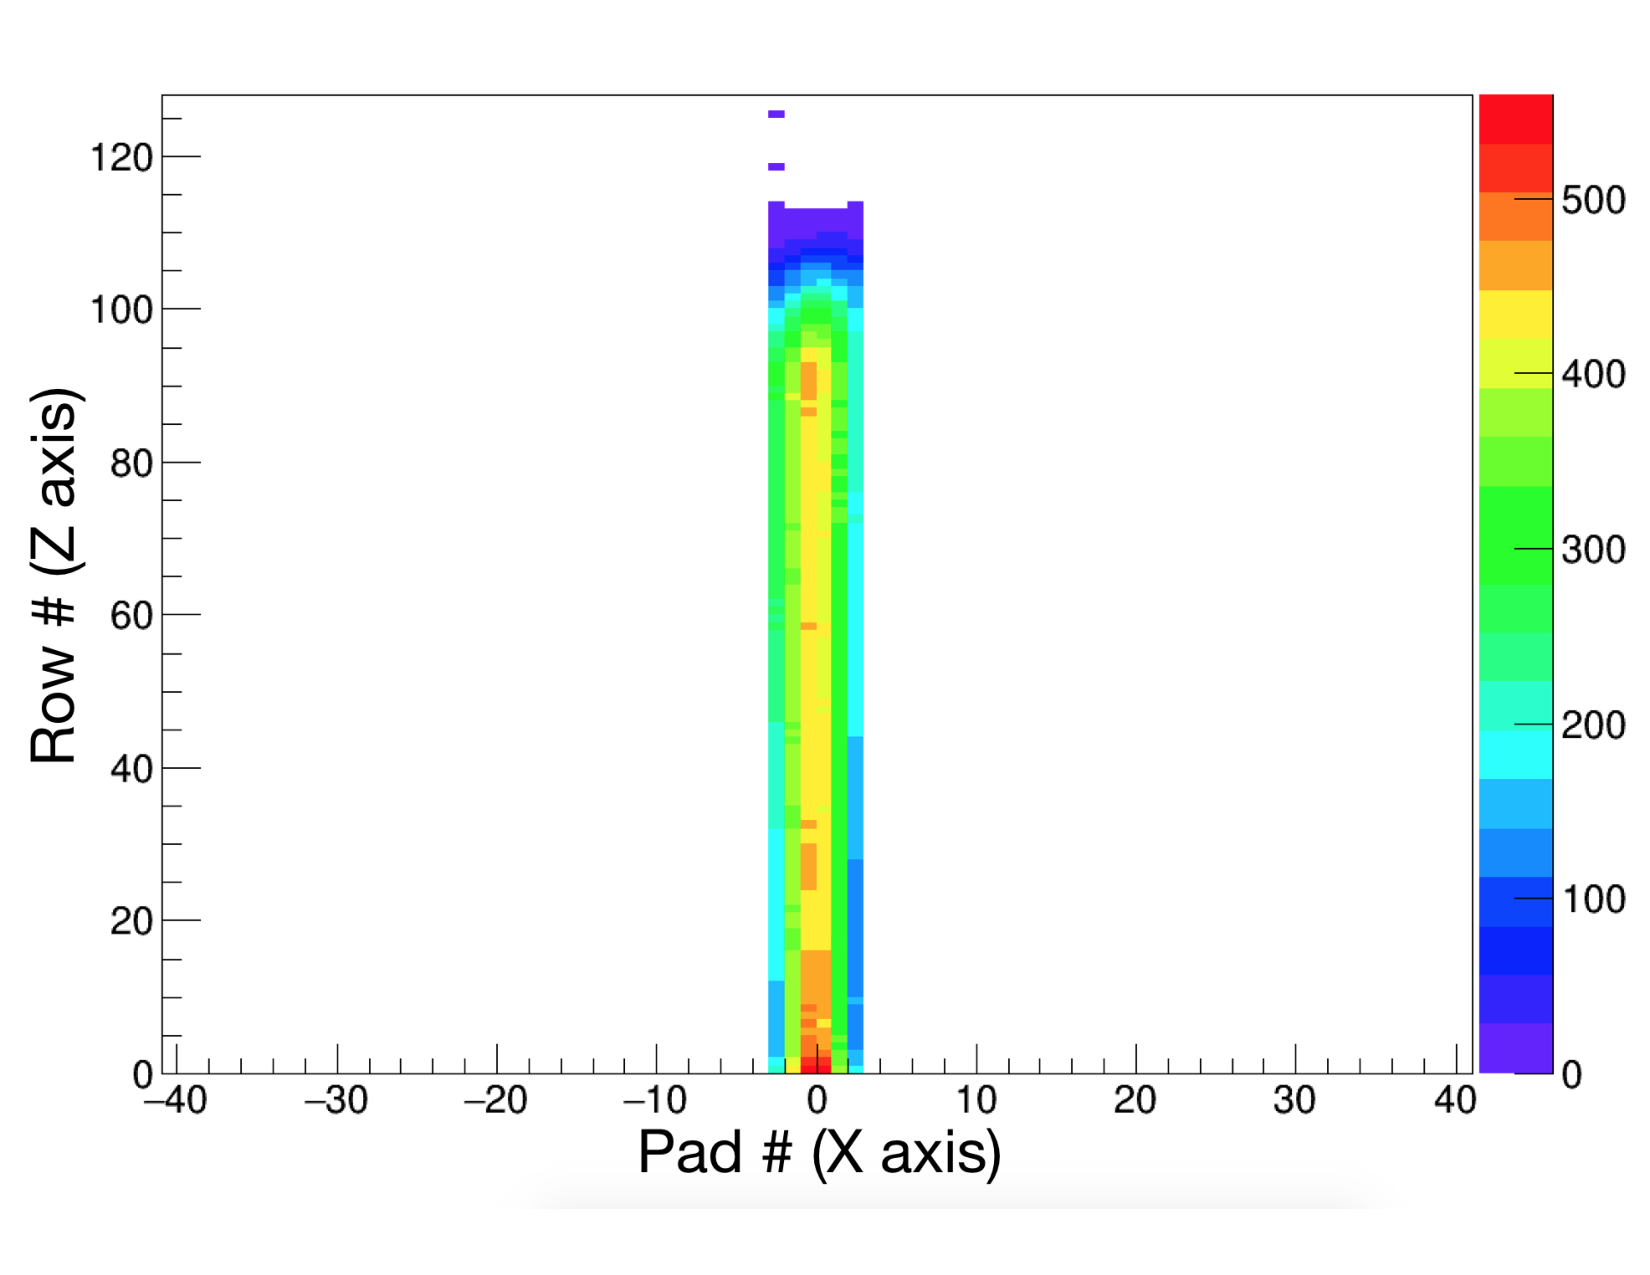
\includegraphics[width=0.5\textwidth]{figures/9CBeamCumulative}
    \caption{The cumulative counts in the central region of the Micromegas for the $^8$B beam. The pressure was adjusted to stop the beam about 1/8th from the end of the Micromegas.}
    \label{fig:9CBeamCumulative}
\end{figure}

\begin{figure}[hbt!]
	\centering
    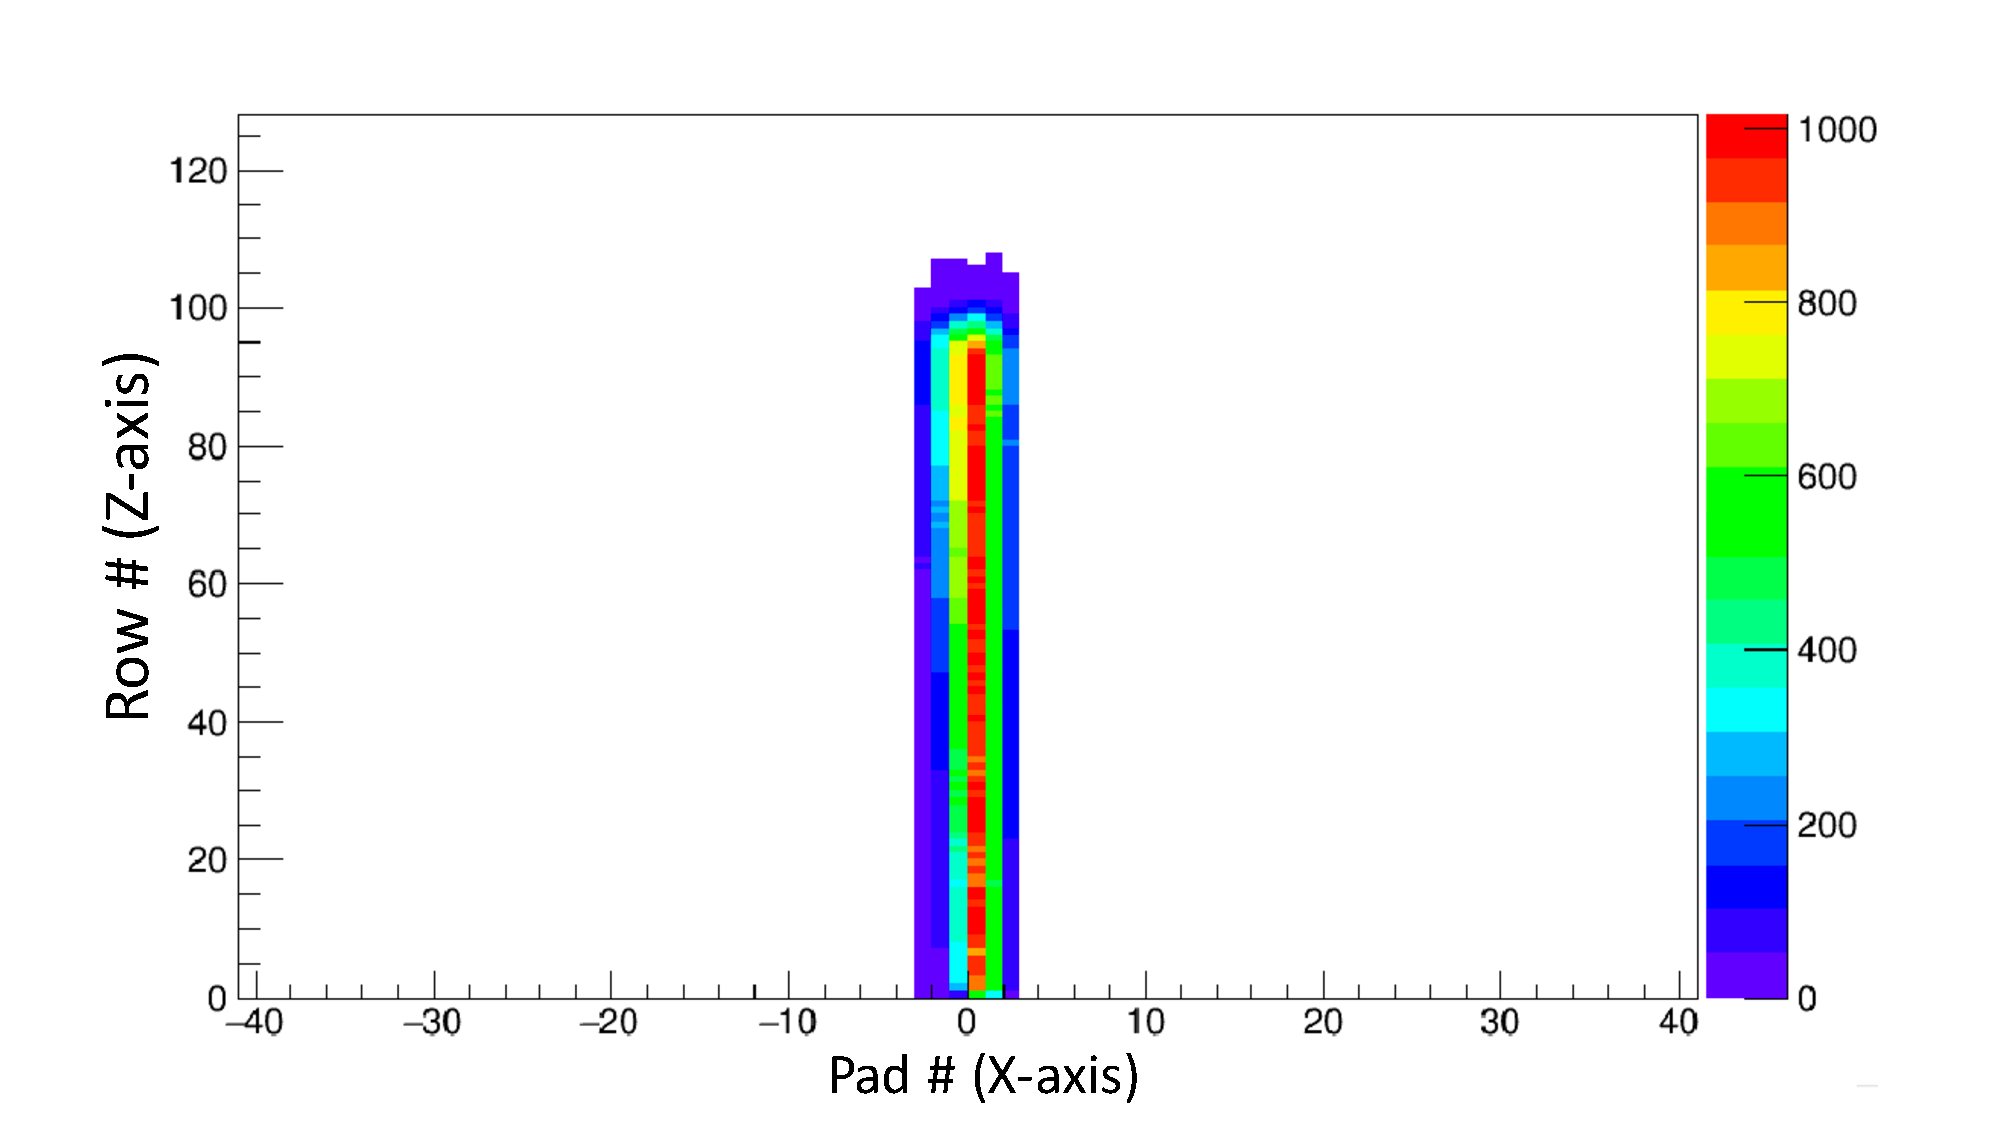
\includegraphics[width=0.5\textwidth]{figures/12CCumulative}
    \caption{The cumulative counts in the central region of the Micromegas for the $^{12}$C beam. The pressure was adjusted to stop the beam about 1/8th from the end of the Micromegas.}
    \label{fig:12CBeamCumulative}
\end{figure}


\begin{figure}[hbt!]
	\centering
    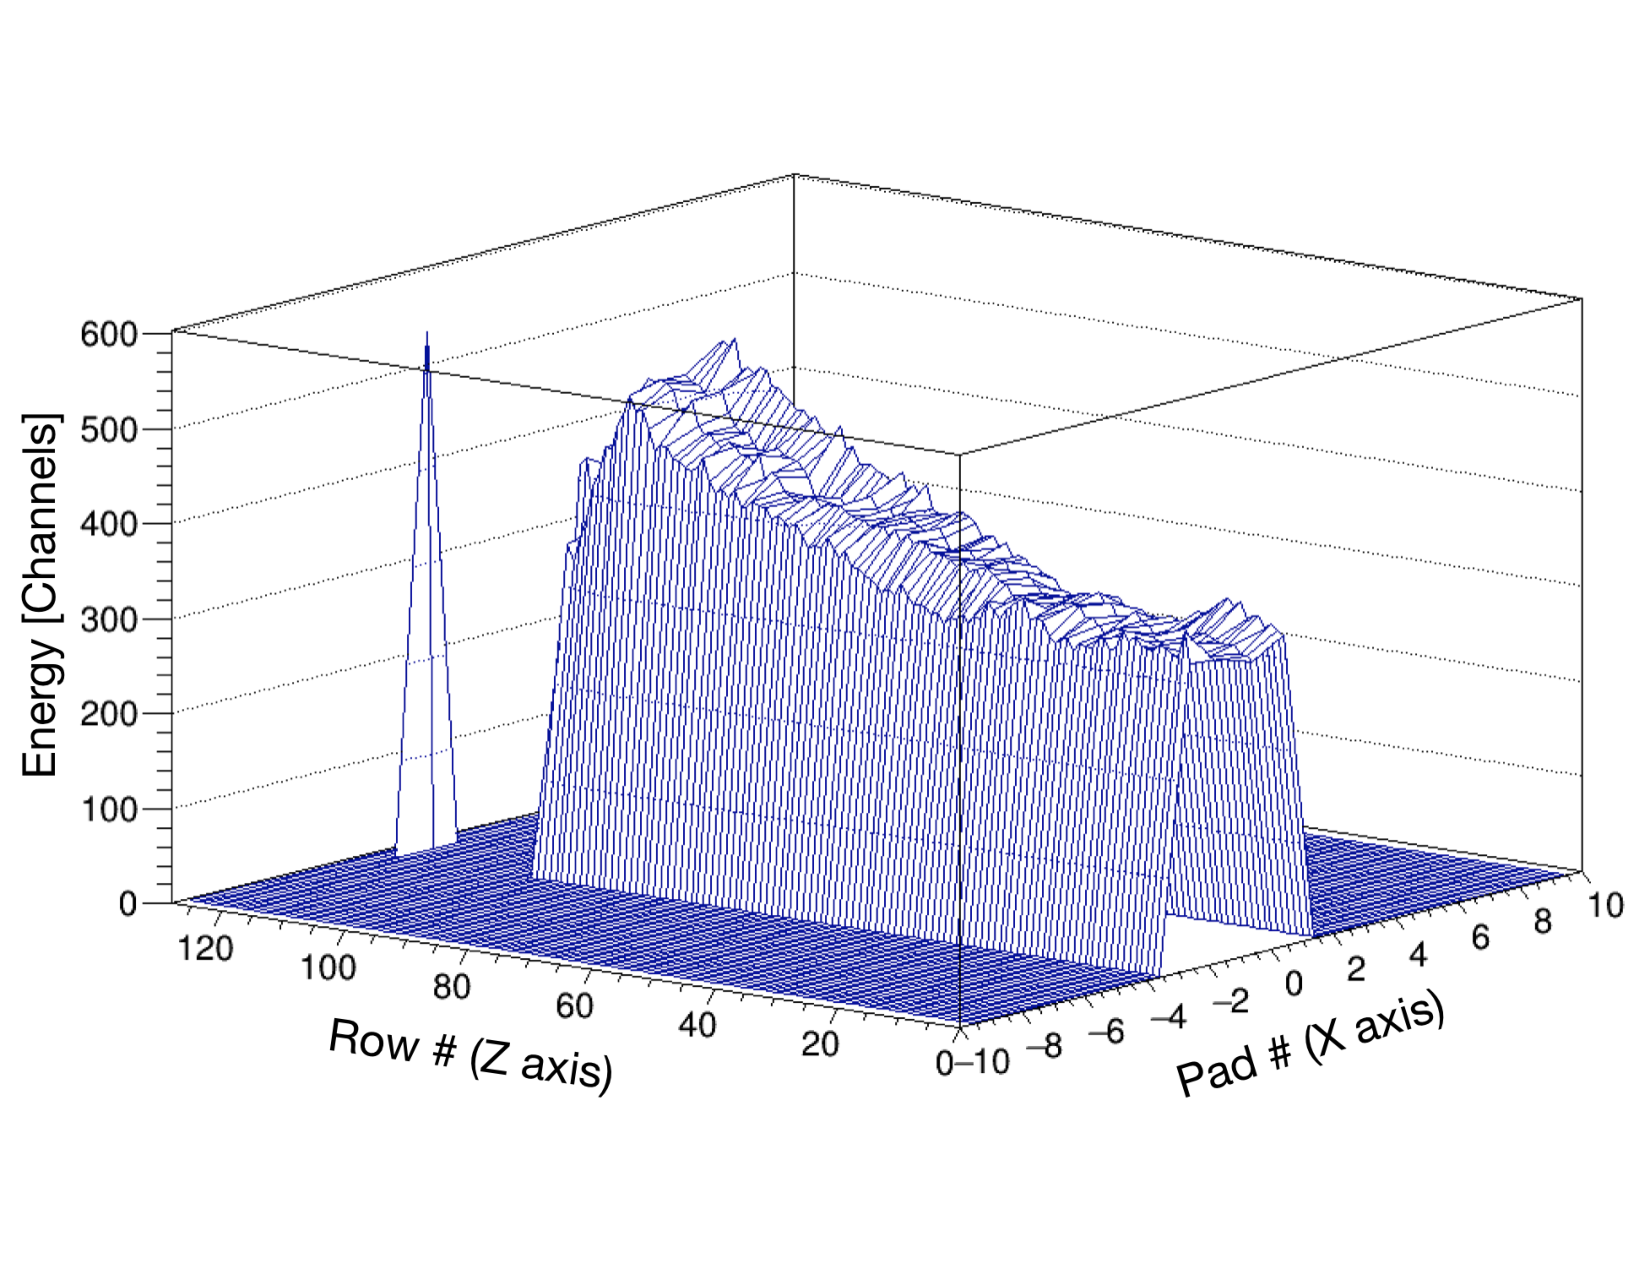
\includegraphics[width=0.5\textwidth]{figures/9CBeamEnergy}
    \caption{The energy deposited in each of the central region pads. The Bragg peak occurs around row number 90.}
    \label{fig:9CBeamEnergy}
\end{figure}

\subsection{Low and High Gain Areas in the Micromegas Detector \label{lowANDhigh}}

The Micromegas detector was split into effectively two regions: one with low gain and another with high gain. The low gain region consists of the first 7/8th of the central pads in the beam direction. This low gain region is used to measure the incoming beam particle and the energy deposition along the pads. It had a Micromegas bias of 400 V. The last 1/8th of the central pad region closest to the Si detectors was biased at 600 V and is a high gain region which was used to measure the protons as the beam is stopped before this region. Both side regions were high gain regions biased at 570 V to obtain the proton tracks.

\subsection{Selecting Proton Events}

To identify proton events, we used the specific energy loss in the high gain regions vs the total energy in the Si and CsI detectors. Since trajectories have variable path length over the active region of Micromegas detector, we use specific energy loss per unit pad for particle ID.The specific energy loss per unit pad for the central detectors plotted against the total energy is shown in Fig. \ref{fig:9C_dEE5}. For the side regions, only the energy deposited in the strips are used to get the specific energy loss since the strips run perpendicular to the beam axis. This means that protons traveling in the forward direction will not skip over any strips nor will the geometry of the pad prevent the full measurement of the energy. The specific energy loss per unit pad plotted against total energy in the side region is shown in Fig. \ref{fig:9C_dEE9}. As shown in both of these figures, protons are easily identified. The protons that punch-through the Si detectors ($>9$ MeV for 700 $\mu$m of Si) produce a signal in the CsI(Tl) providing additional identification shown in Fig. \ref{fig:TexAT_SiECsIE}.

The gap in Fig. \ref{fig:9C_dEE5} between $\sim 9$ and $\sim 10$ MeV corresponds to the threshold in the CsI detectors. The protons in this energy region do not deposit enough energy in the CsI to be recorded due to the threshold for the CsI(Tl) channels in GET electronics. This threshold can actually be eliminated if complete readout mode is used in GET, in which case the ``threshold'' would be defined by the CsI(Tl) noise level. However, it was not done in the commissioning run. Shown in Fig. \ref{fig:TexAT_SiECsIE} is the Si energy plotted against the energy deposition in the corresponding CsI(Tl). As shown, we start recording a signal in the CsI detector when the punch-through protons are only depositing less than 7.5 MeV in the Si detector.

\begin{figure}[hbt!]
	\centering
    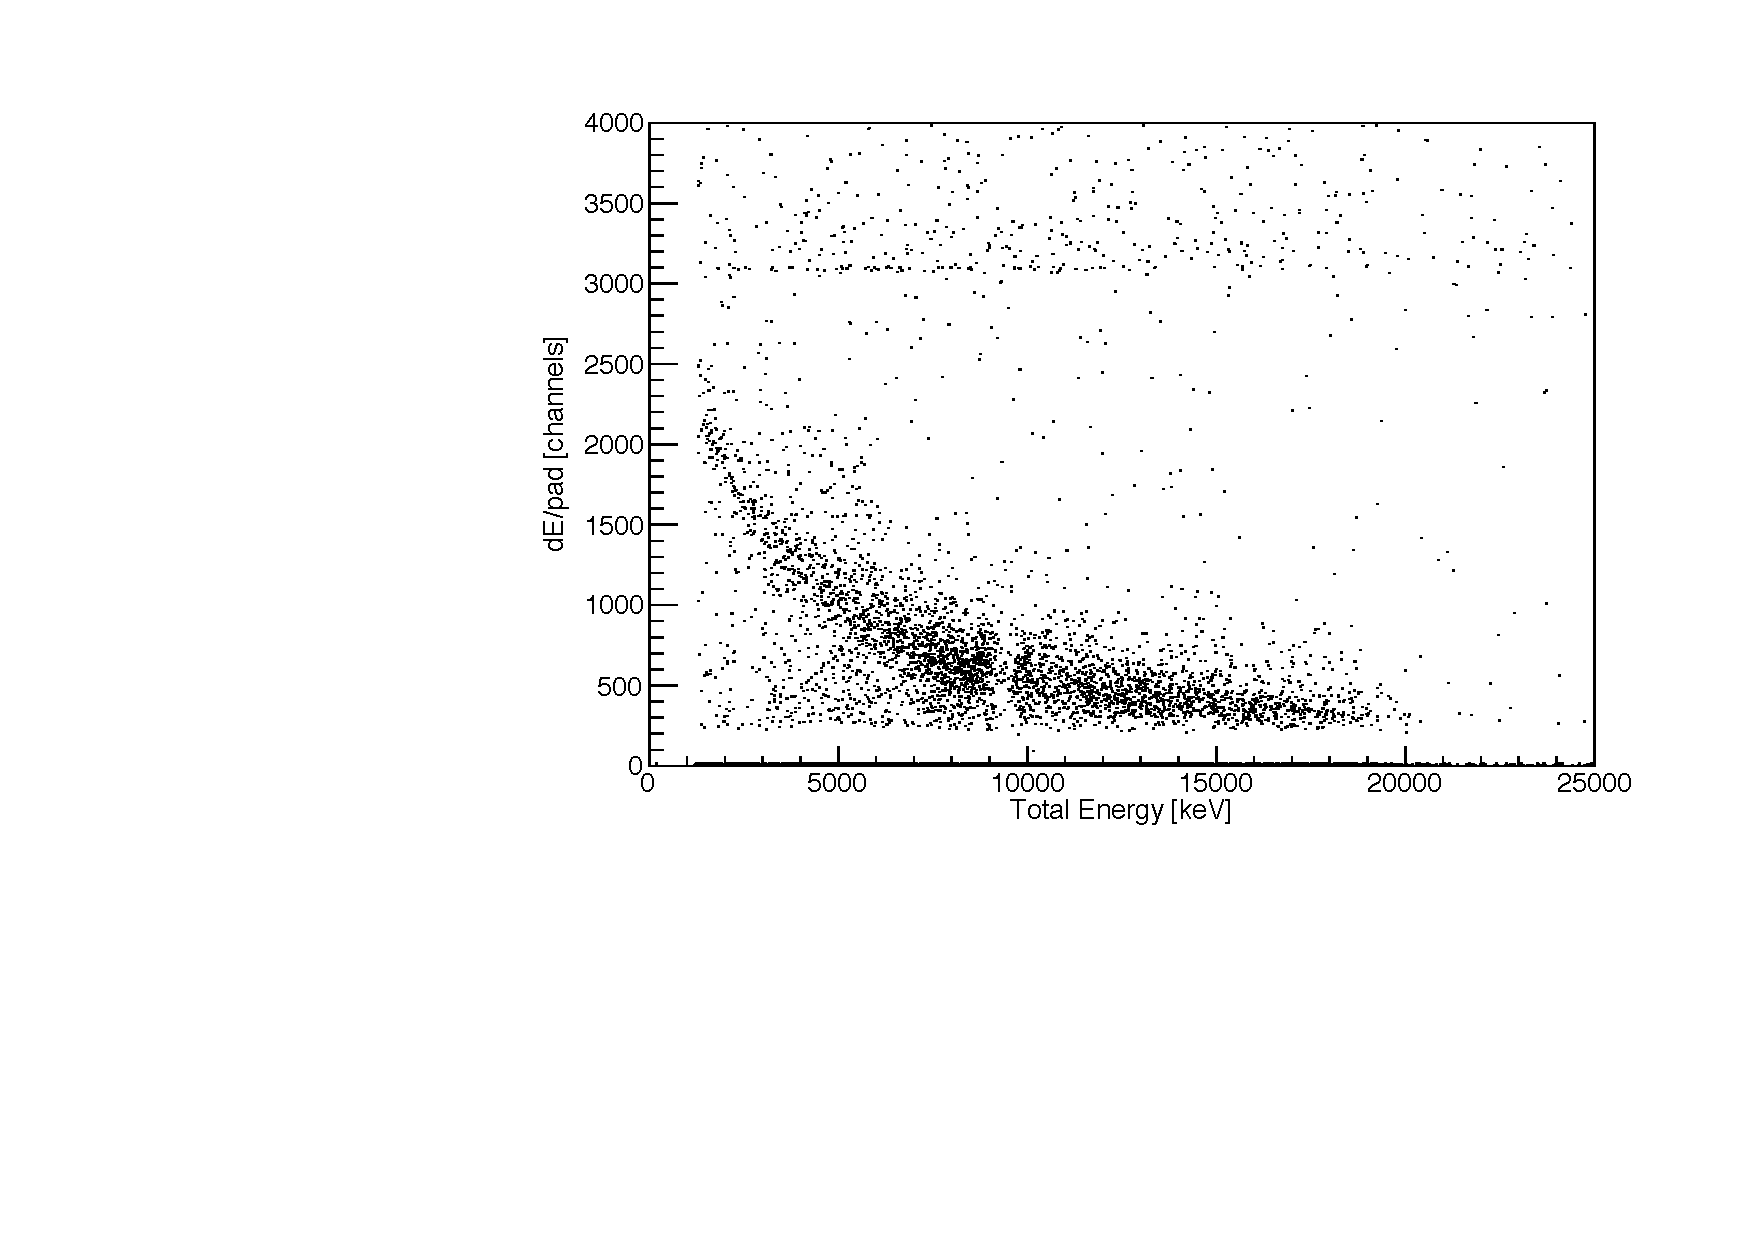
\includegraphics[width=0.5\textwidth]{figures/9C_dETotalE_d5}
    \caption{The specific energy loss per unit pad in the central region plotted against the total energy measured in the Si and CsI detector. The energy loss is measured in the last 1/8th in the central pads.}
    \label{fig:9C_dEE5}
\end{figure}

\begin{figure}[hbt!]
	\centering
    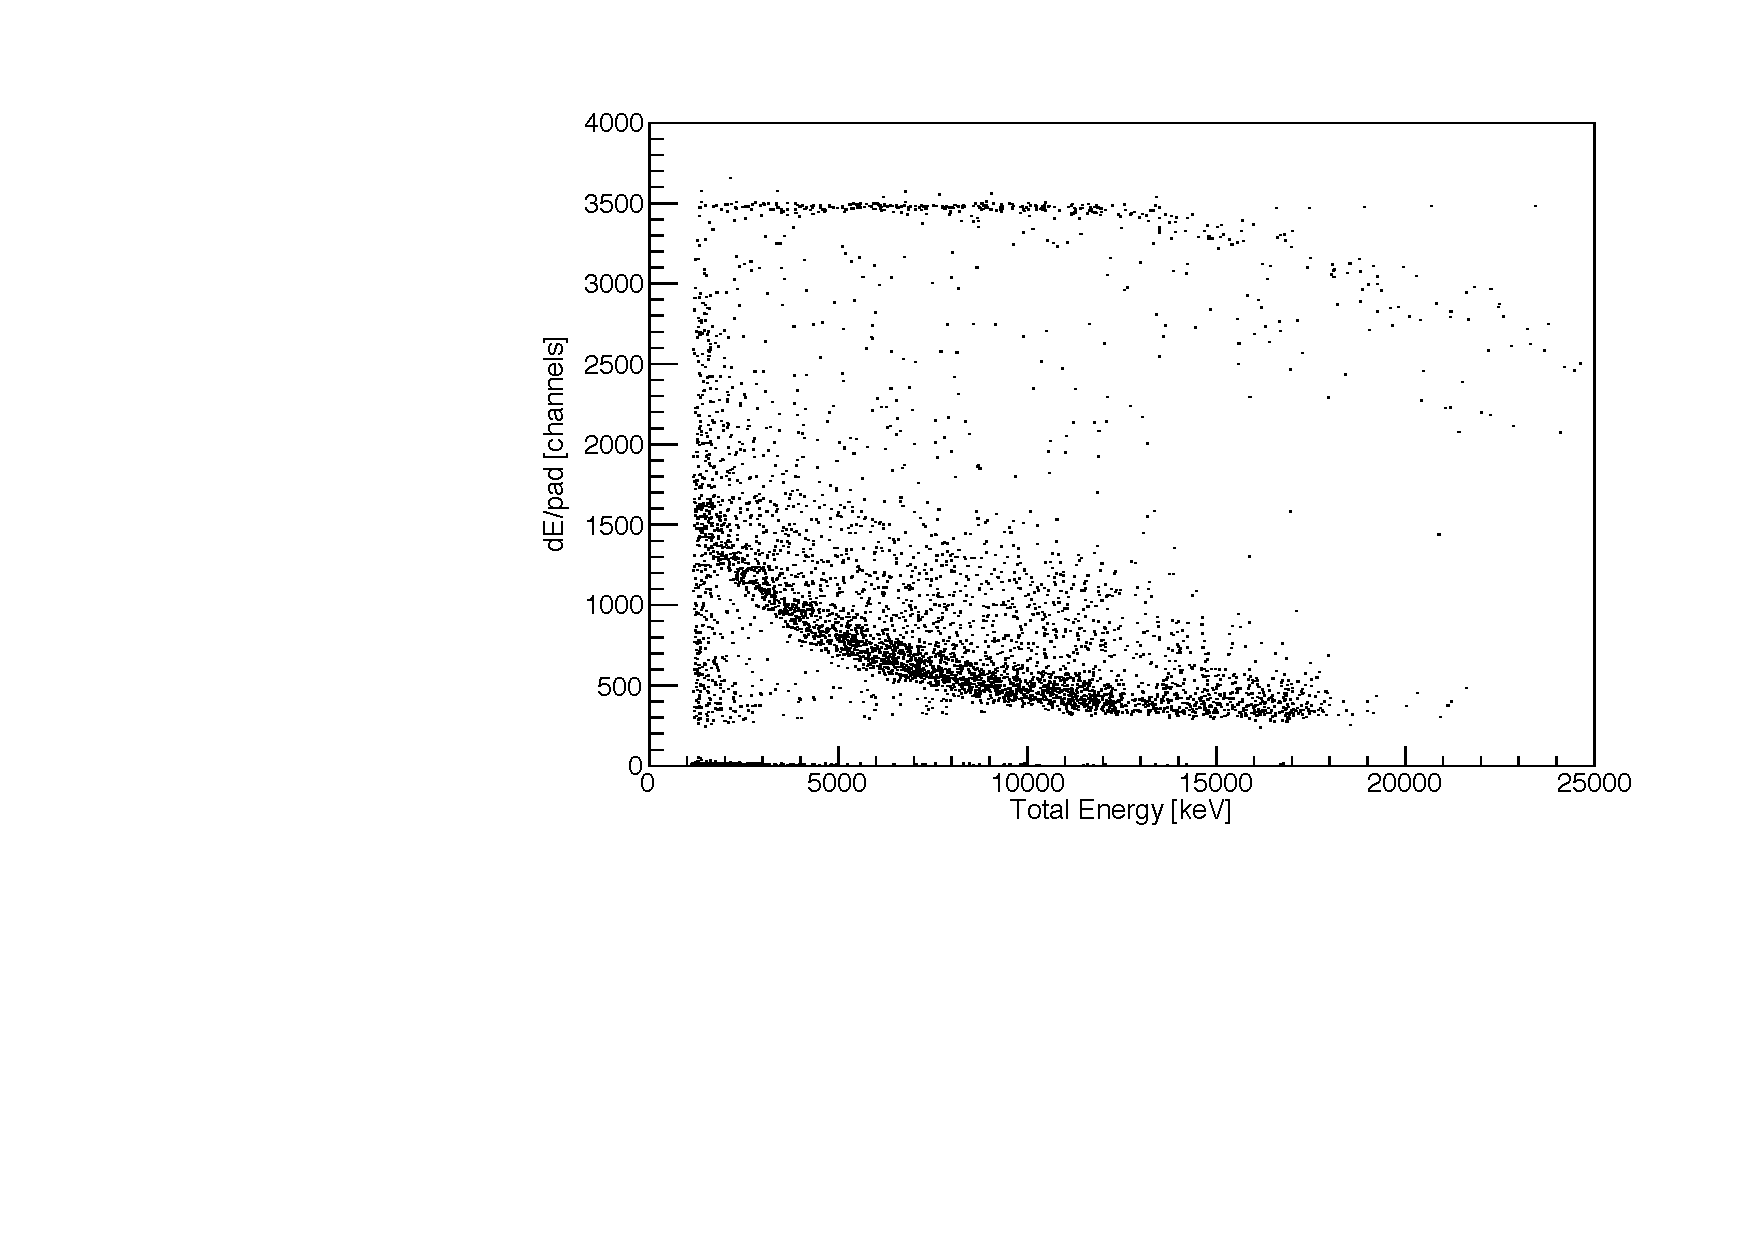
\includegraphics[width=0.5\textwidth]{figures/9C_dETotalE_d9}
    \caption{The specific energy loss per unit pad of the strips in the side region plotted against the total energy measured in the Si and CsI detector.}
    \label{fig:9C_dEE9}
\end{figure}

\begin{figure}[hbt!]
	\centering
    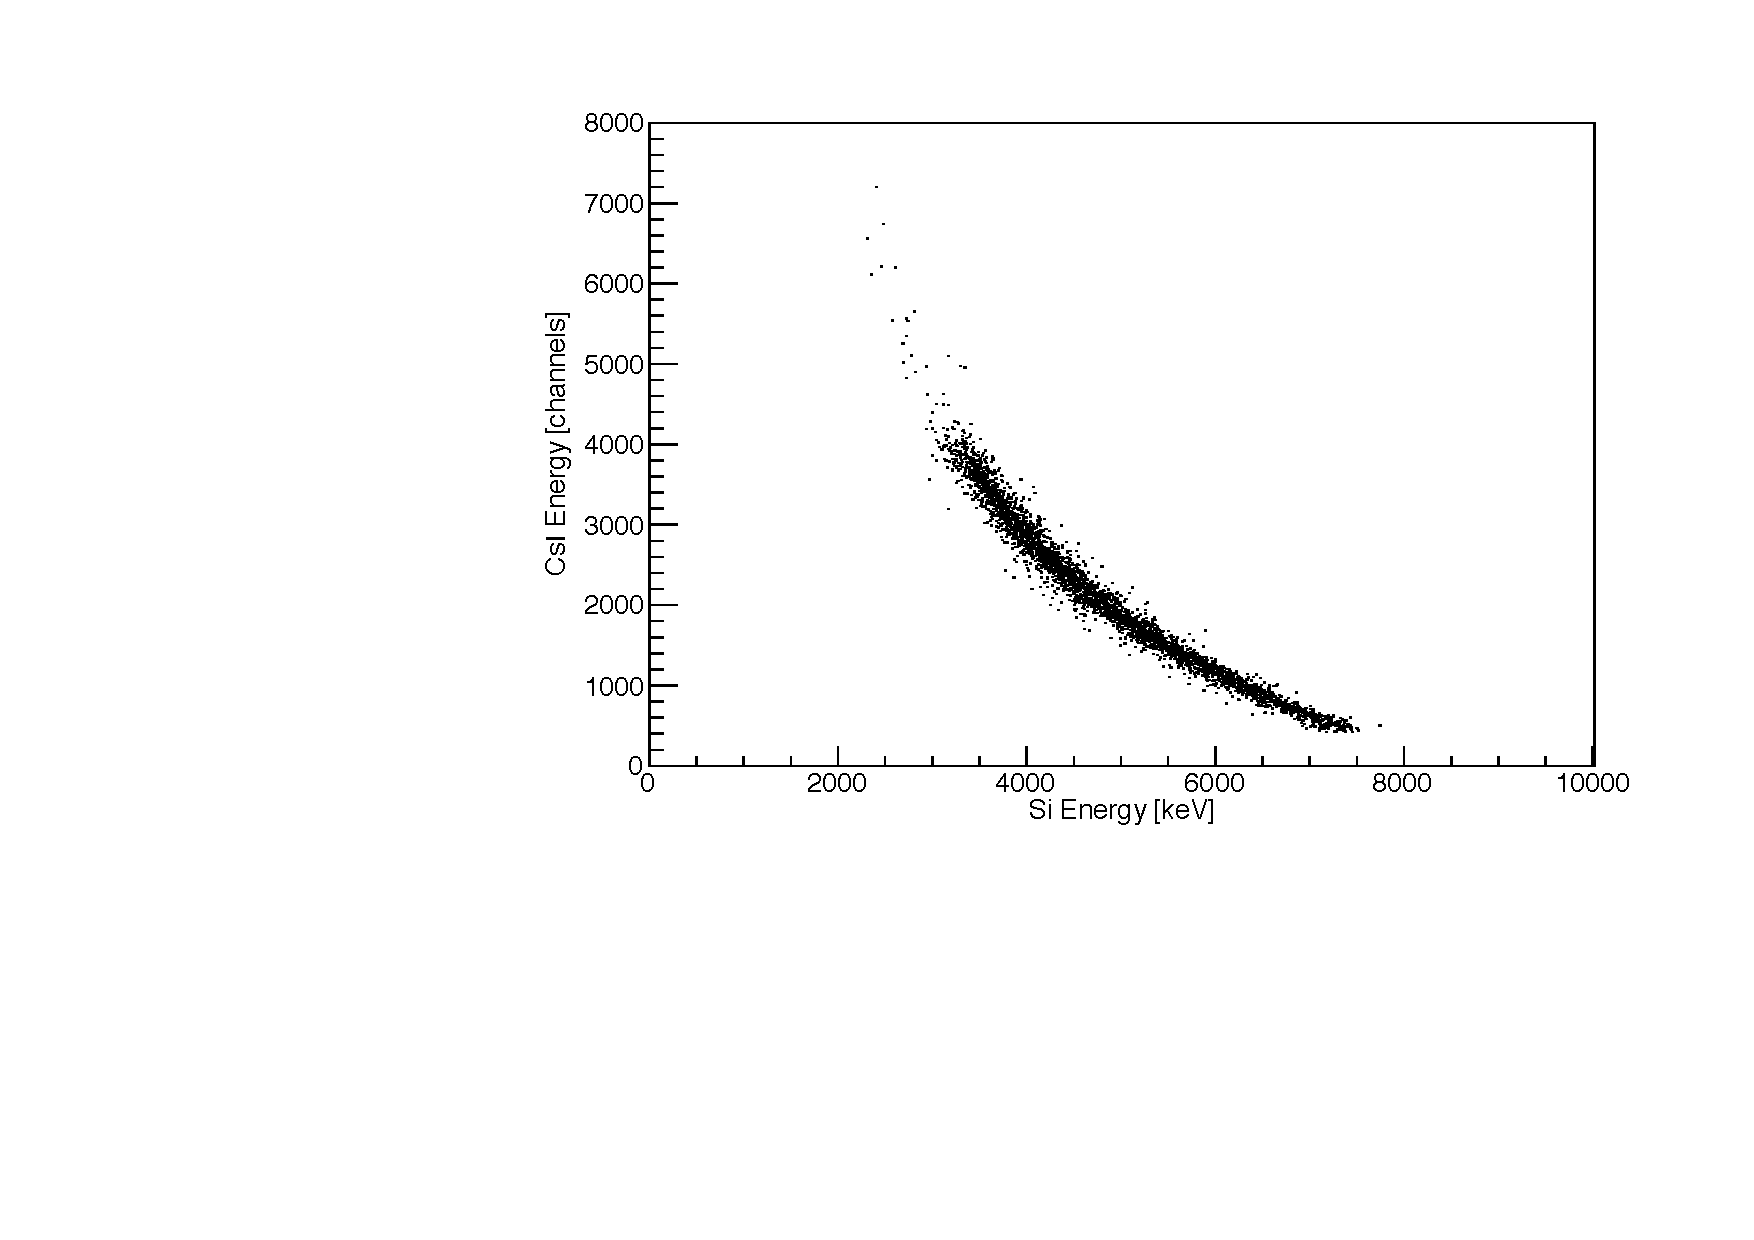
\includegraphics[width=0.5\textwidth]{figures/TexAT_SiECsIE}
    \caption{The energy recorded in the CsI detector in channel number plotted against the measured energy(in keV) in the Si detector.}
    \label{fig:TexAT_SiECsIE}
\end{figure}

\subsection{Identification of inelastic scattering events}

The main focus of the commissioning run was excitation function for $^8$B+p resonance elastic scattering. However, inelastic scattering events were clearly observed. There are no proton-bound excited states in $^8$B because its protons decay threshold is located at 137 keV and the first excited states (1$^+$) is at 770 keV. As a result, any inelastic scattering event will produce two protons and a $^7$Be recoil (which itself may be in its ground or excited state). By looking for the events with two proton tracks, we can identify these inelastic scattering events.

Using the total energy in the Si and CsI detectors and the Micromegas, we can clearly identify protons that hit one of the Si detectors and triggered the DAQ, but ``second'' protons produced by an inelastic scattering event do not always hit any Si detector. Therefore, we cannot rely on specific energy loss vs the total measured energy and need to identify protons by only using their tracks in the gas. Specific energy loss of Z=1 nuclei is very different from that of heavier recoils (e.g. $^7$Be) and there appears to be no or very few deuterons or tritons produced in the interaction of $^8$B with the methane gas (see Fig. \ref{fig:9C_dEE5} and \ref{fig:9C_dEE9}). So, by comparing specific energy loss per unit pad we can determine if the particle is a heavy recoil or a proton. Examples of protons measured in the side regions and the second proton is measured in the central region (Figure \ref{fig:9C_Inelastic_Center}) and opposite side region (Figure \ref{fig:9C_Inelastic_Side}) are shown. By identifying these events, we are able to exclude them from the excitation function for resonance elastic scattering. The excitation function for inelastic scattering can also be constructed from this data, but it was not in the scope of this work.

\begin{figure}[hbt!]
	
  		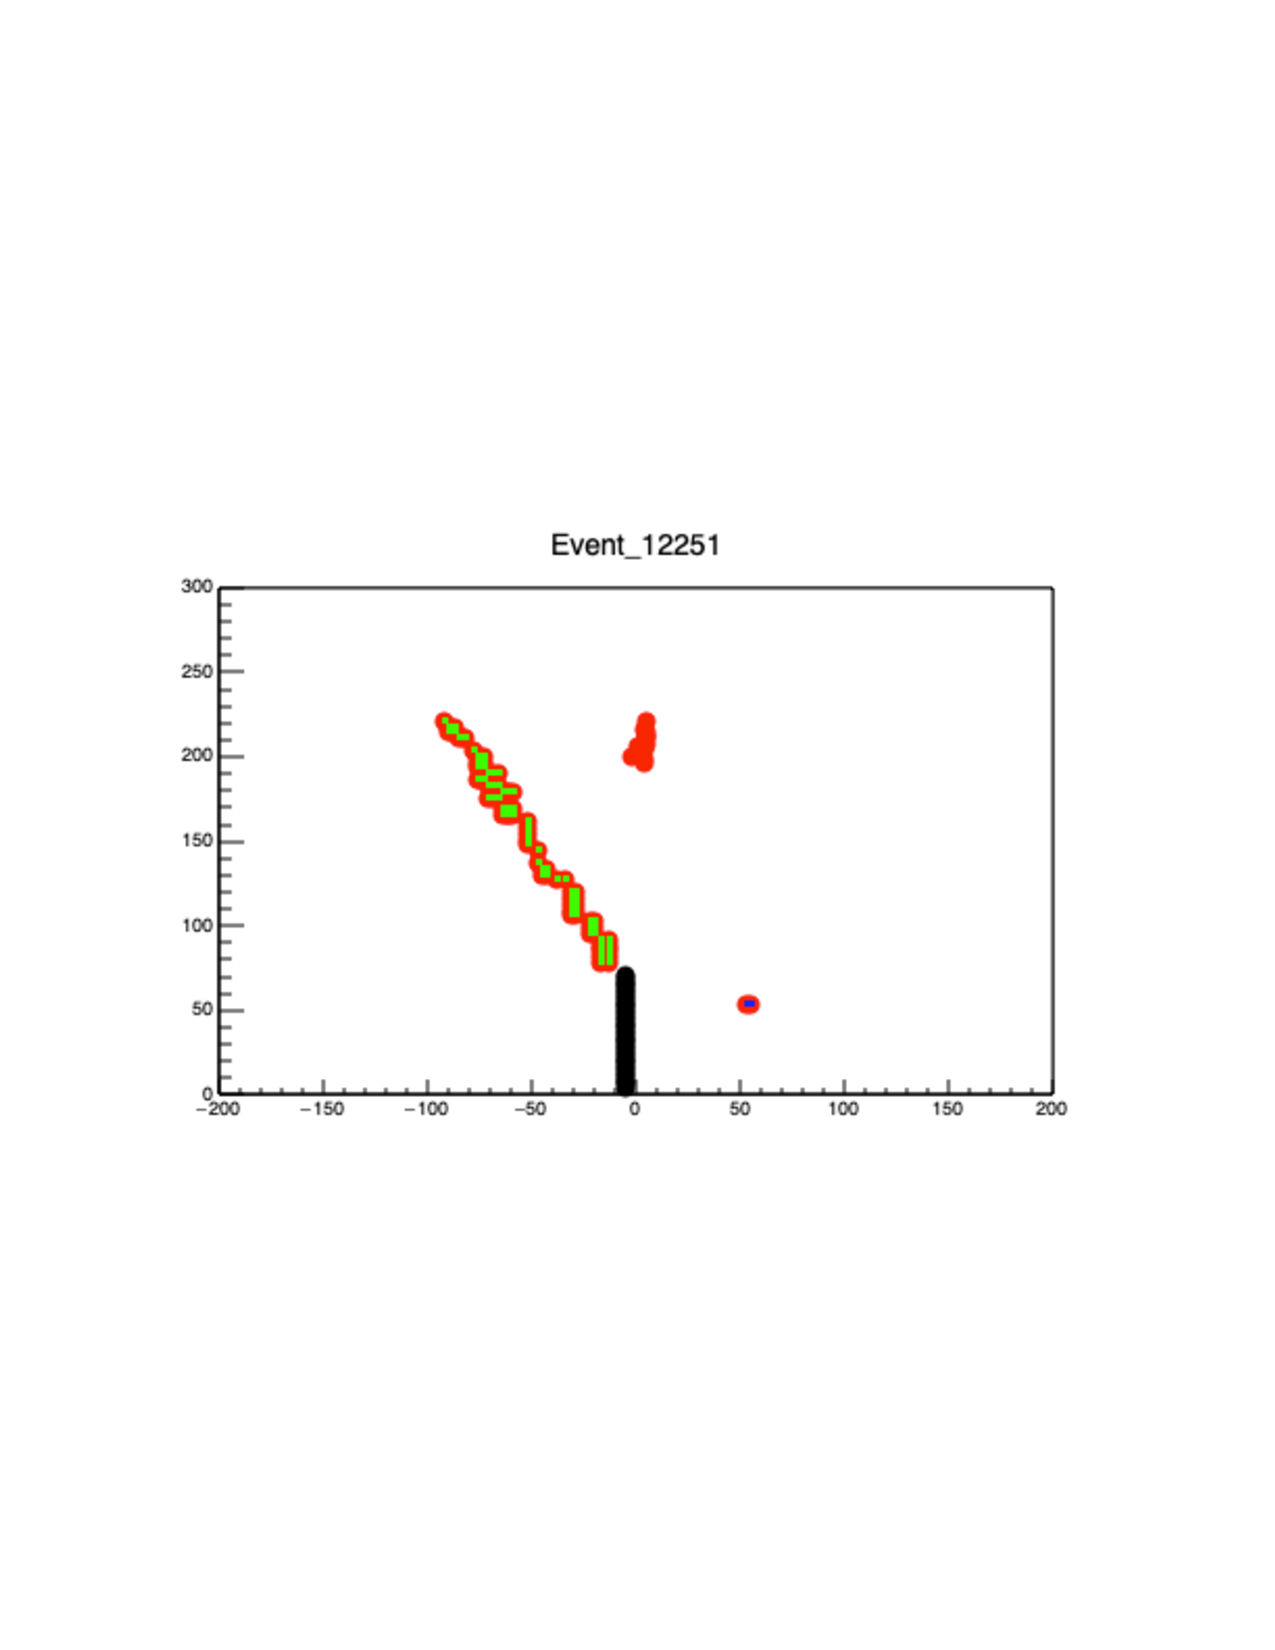
\includegraphics[width=1.0\linewidth]{figures/9C_Inelastic_Central_1}

  		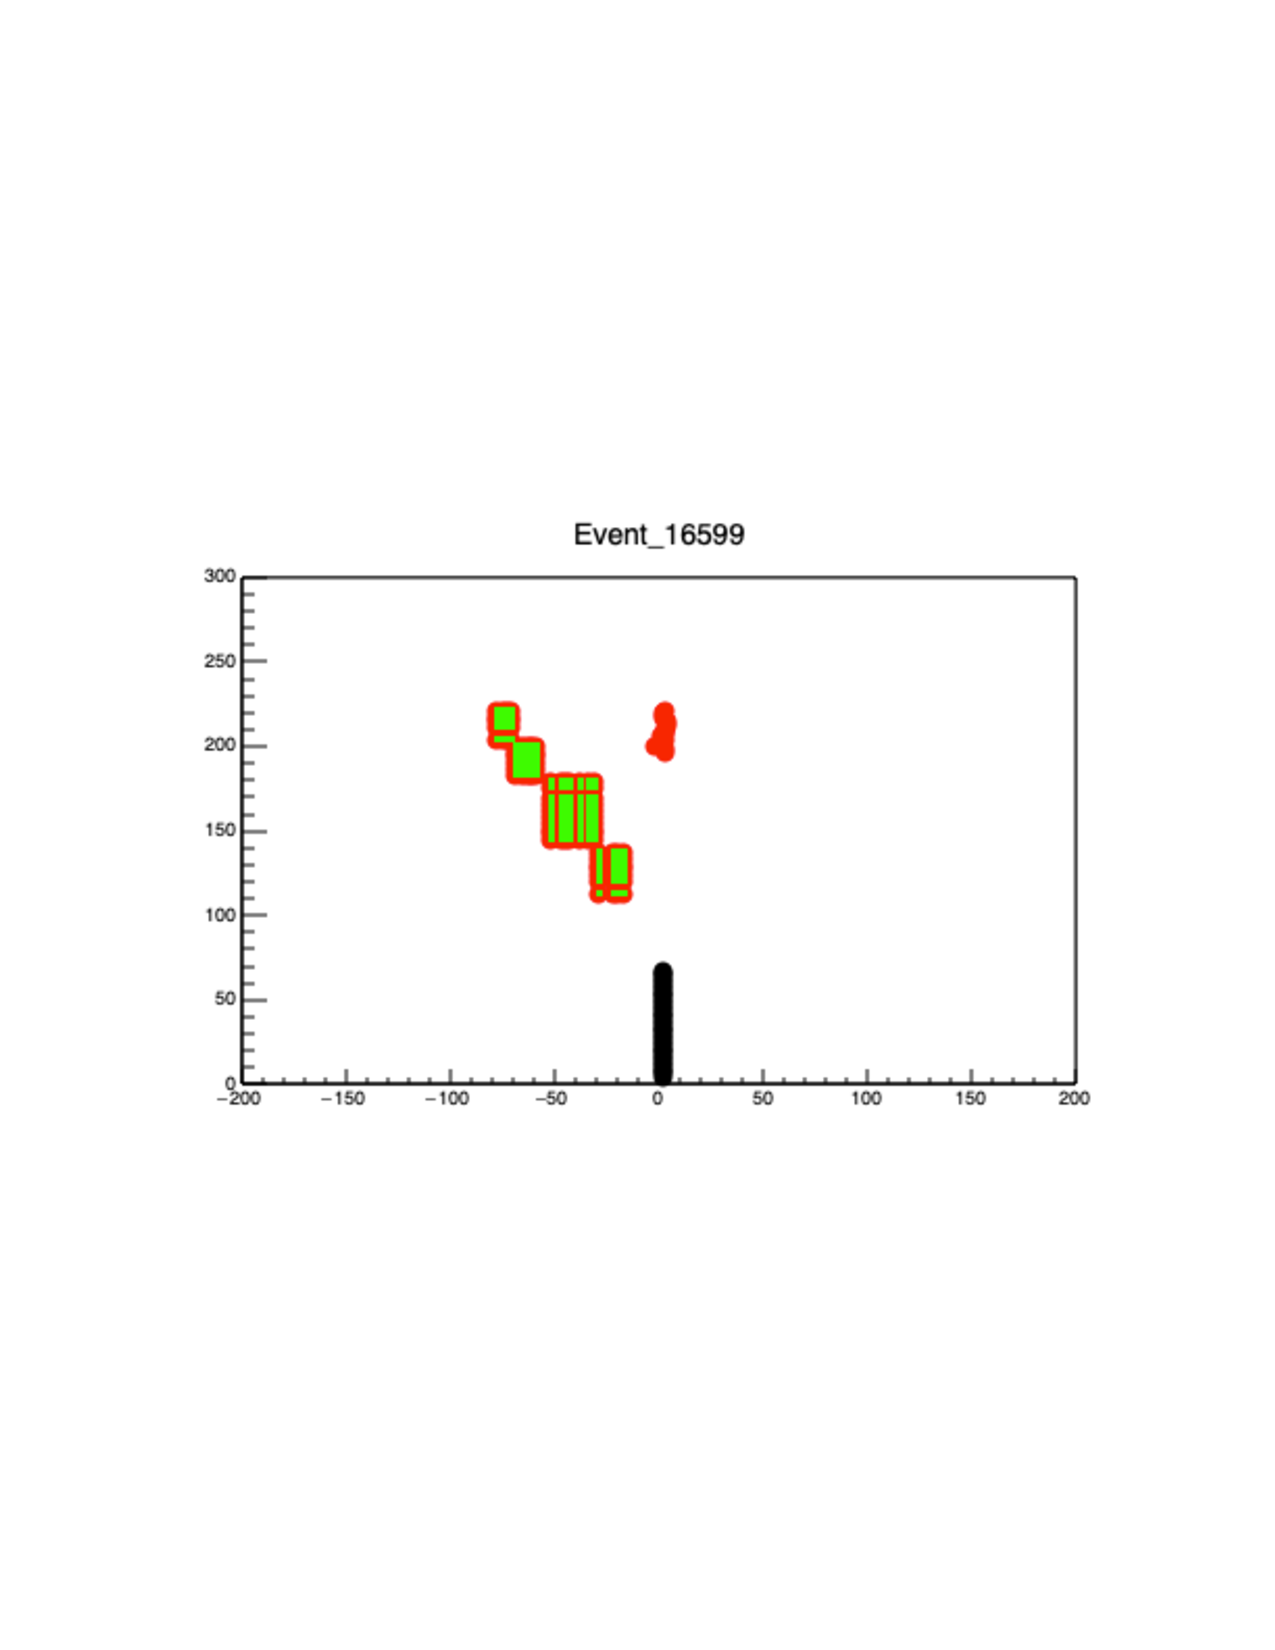
\includegraphics[width=1.0\linewidth]{figures/9C_Inelastic_Central_2}

	\caption{Inelastic events where a proton is measured one side of the Micromegas plate and a proton in the central region.}
	\label{fig:9C_Inelastic_Center}
\end{figure}

\begin{figure}[hbt!]
	  
	  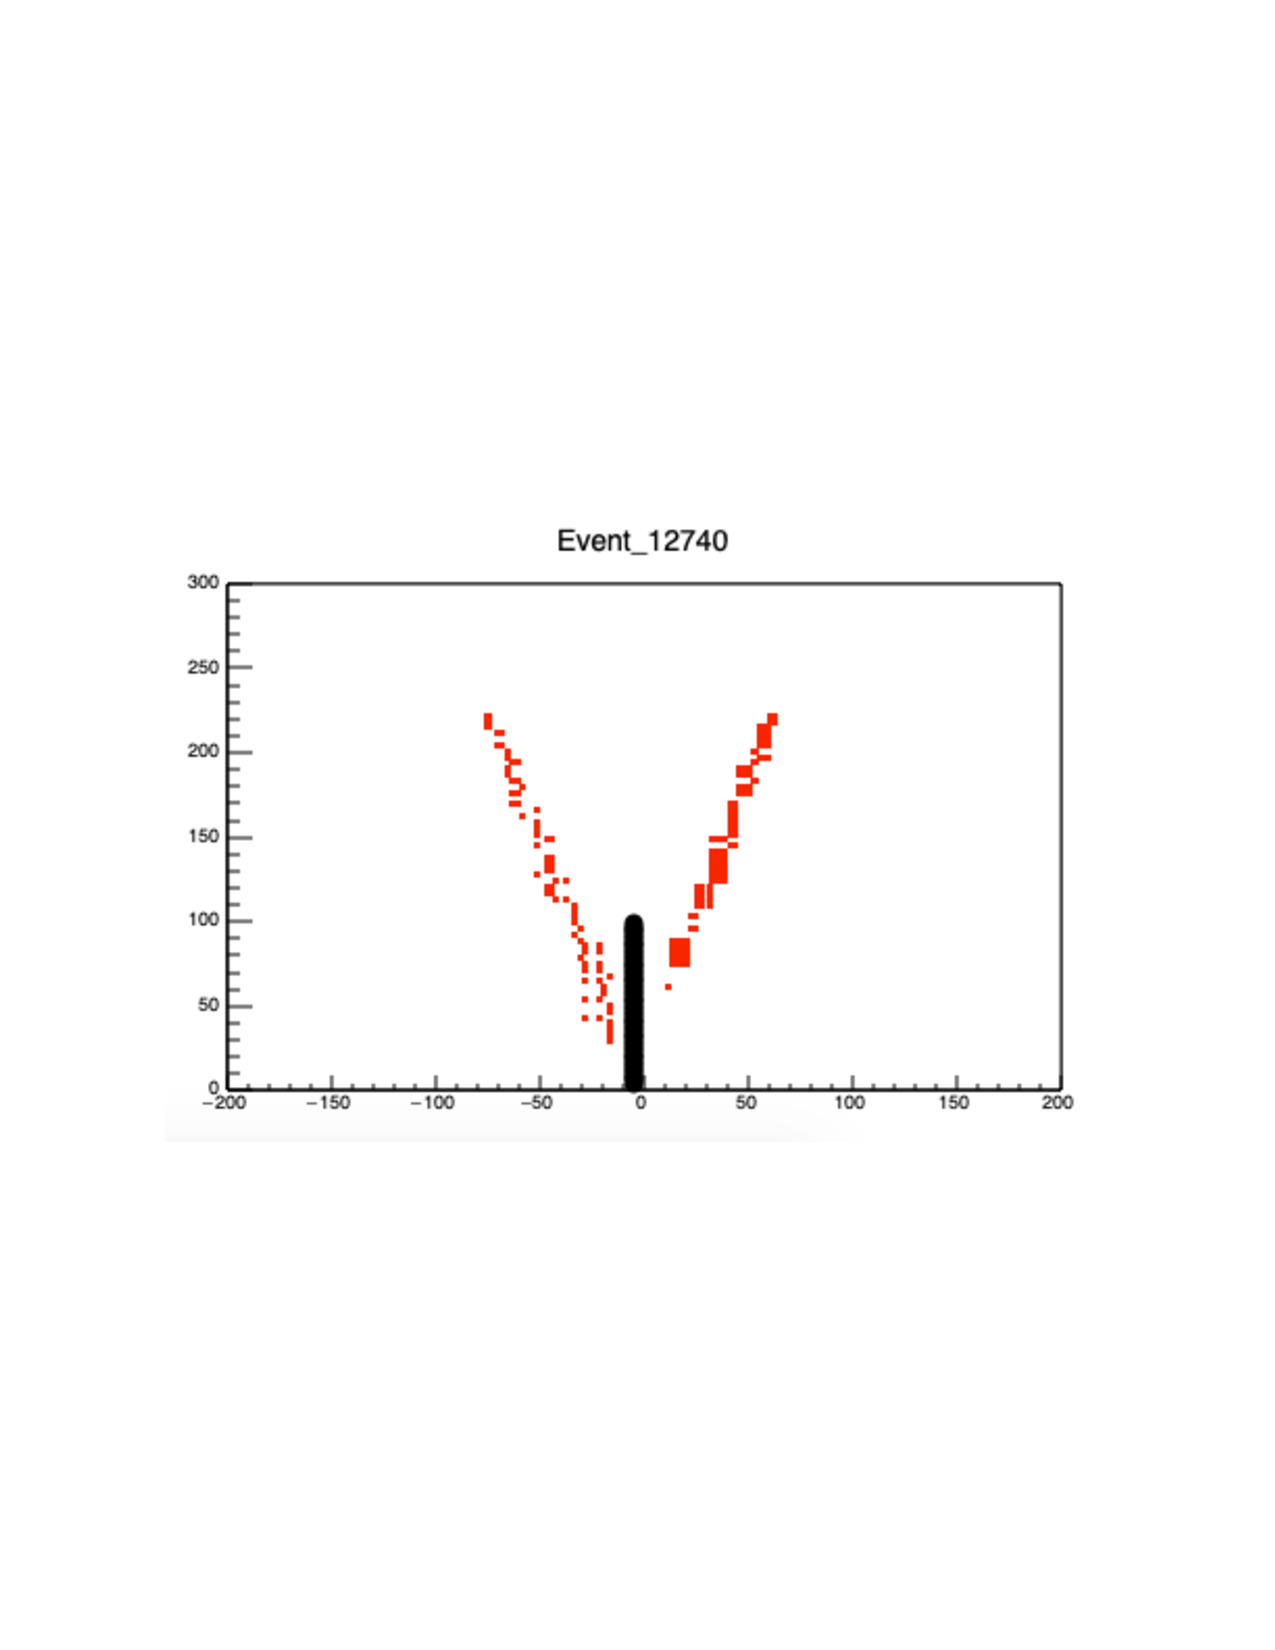
\includegraphics[width=\linewidth]{figures/9C_Inelastic_Event_1}
	  
   	  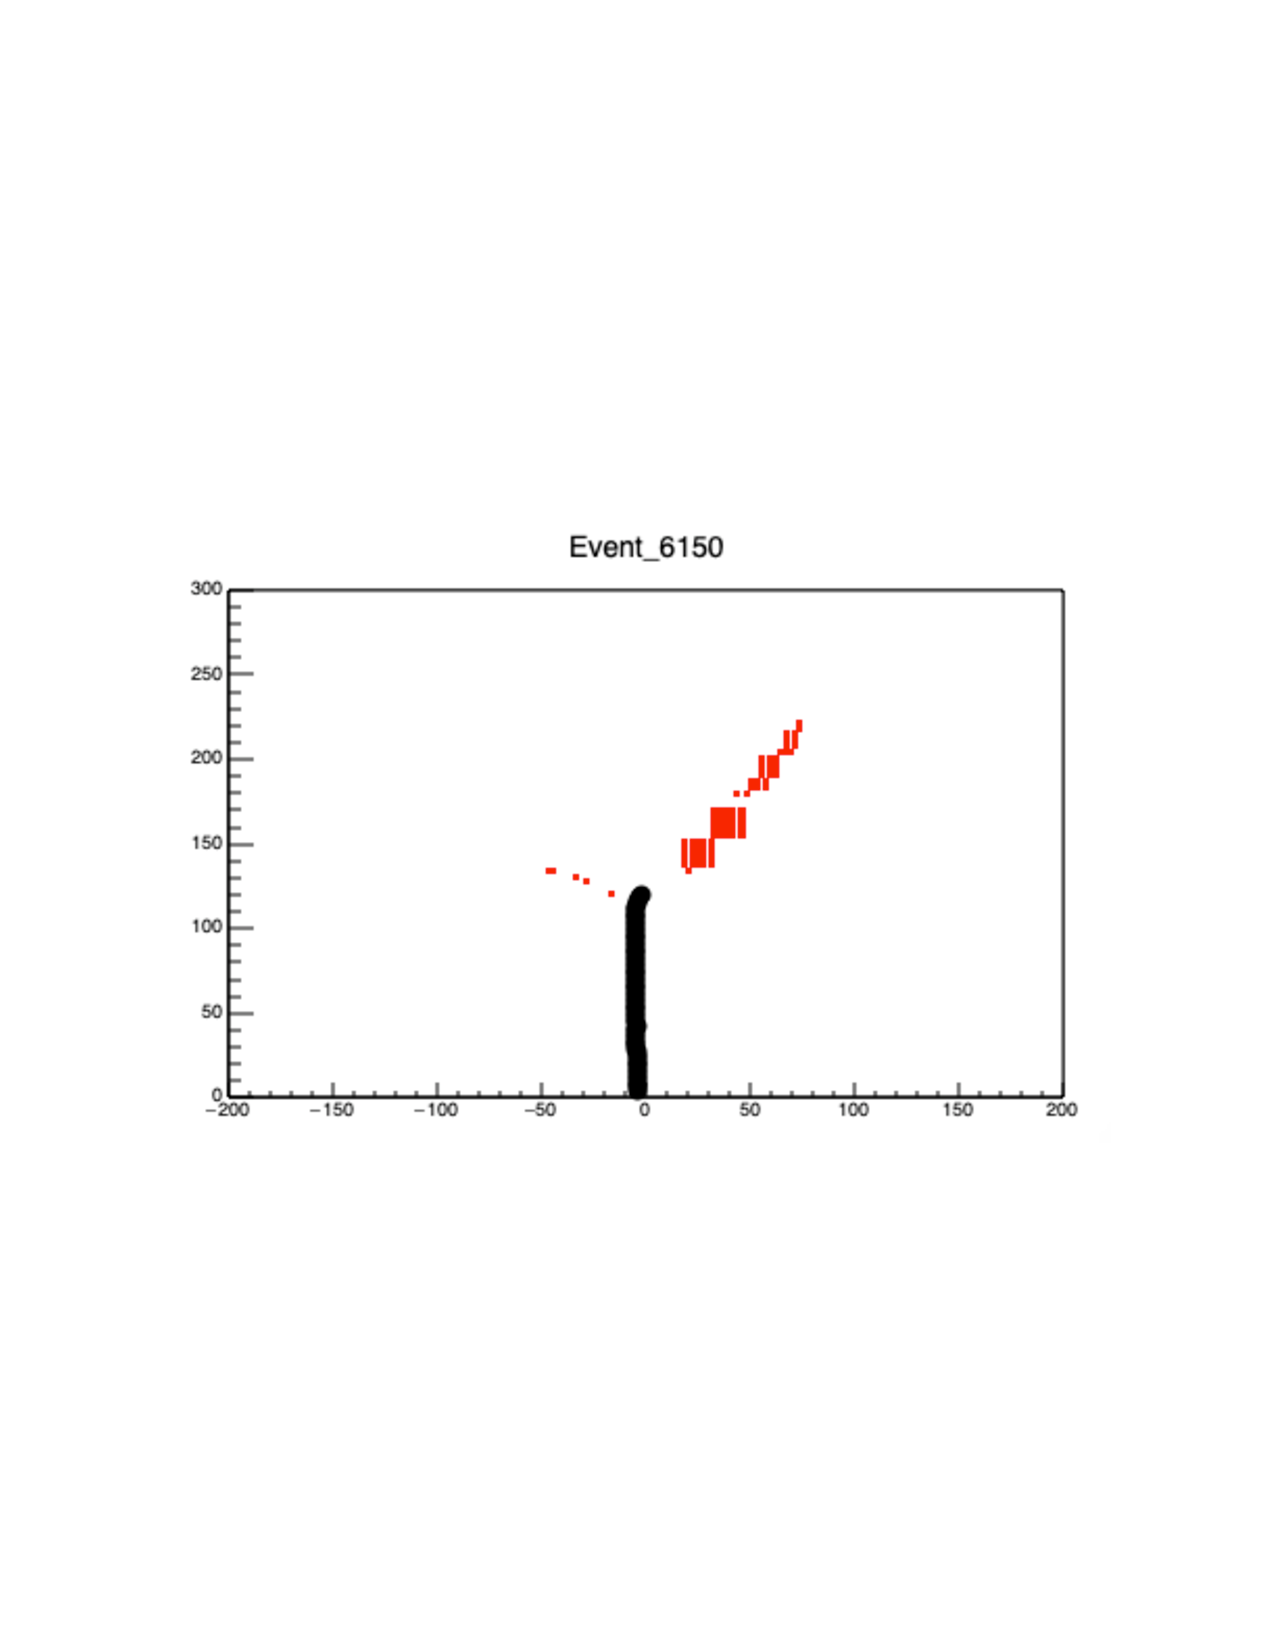
\includegraphics[width=\linewidth]{figures/9C_Inelastic_Event_2}

	\caption{Inelastic events where protons are measured in both sides of the Micromegas plate.}
	
	\label{fig:9C_Inelastic_Side}
	
\end{figure}

\subsection{Vertex Reconstruction in the Central Region}

The following procedure is used for reconstruction of the event kinematics in the central region.
As the $^{8}$B beam propagates over the active region of Micromegas, it deposits energy by ionizing gas in the region of central pads. When a reaction occurs over the Micromegas, such as elastic proton scattering, the energy deposition changes. At this reaction point, there is a jump in specific energy loss because $^{8}$B ion transfers a fraction of its energy to the target proton and therefore specific energy loss changes instantaneously at the interaction point. This sudden energy change can be directly observed in the pads as long as the vertex is over the Micromegas. In this measurement, only events below $E_{c.m.} = 3.2$ MeV will have a vertex position over the Micromegas plate. An alternative way to determine the vertex location for central events and for events produced at c.m. energies above $3.2$ MeV is to identify the location of the Bragg peak for a heavy recoil. Since the elastically scattered proton events measured in the central detectors travel at angles close to zero degrees, the heavy recoil also travels at angles close to zero (due to momentum conservation). This heavy recoil is then measured completely over the central pad region of the Micromegas. The energy of the heavy recoil produced in the $^8$B+p elastic scattering depends on the location of the interaction or c.m. energy. These scattered recoils with higher energies travel further through the gas and the location of the Bragg peak can be measured. Two typical events of this kind are shown in Figure \ref{fig:9C_Center_Energy_Deposition}. By using kinematics and energy loss, we can formulate a way to relate the maximum energy deposition in the Micromegas with the vertex location. This is used to determine the vertex position for the events that produced a proton in the central region. The vertex position determined this way is plotted against the total energy measured in the Si and CsI in Fig. \ref{fig:9C_VertexReconstructionRegion1}. As expected, the vertex position is further away from the Si detectors (vertex position going further negative) as the total energy becomes higher. This figure demonstrates that vertex location can be reliably identified even if an interaction occurs outside of the active region of Micromegas (negative values along the y axis in Fig. \ref{fig:9C_VertexReconstructionRegion1}).

\begin{figure}[hbt!]
  		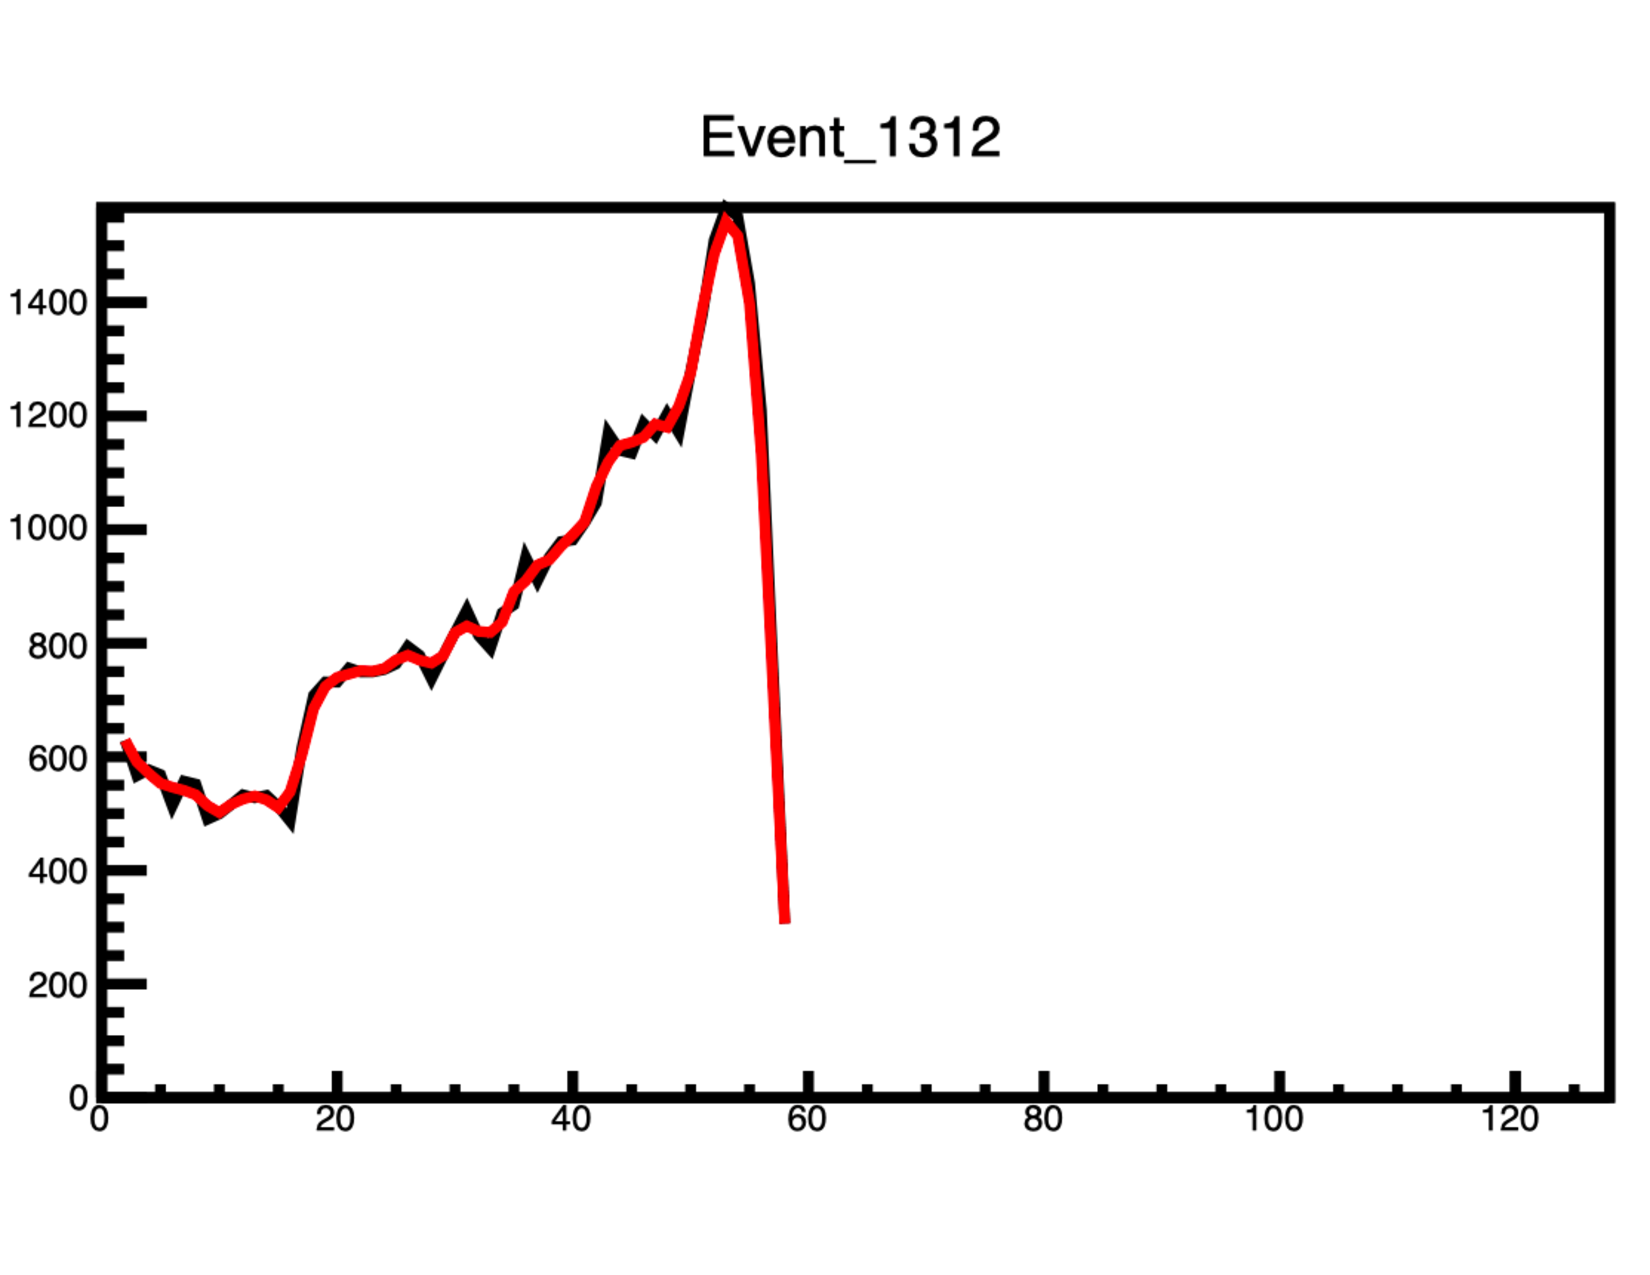
\includegraphics[width=\linewidth]{figures/9C_Center_Energy_1}
  		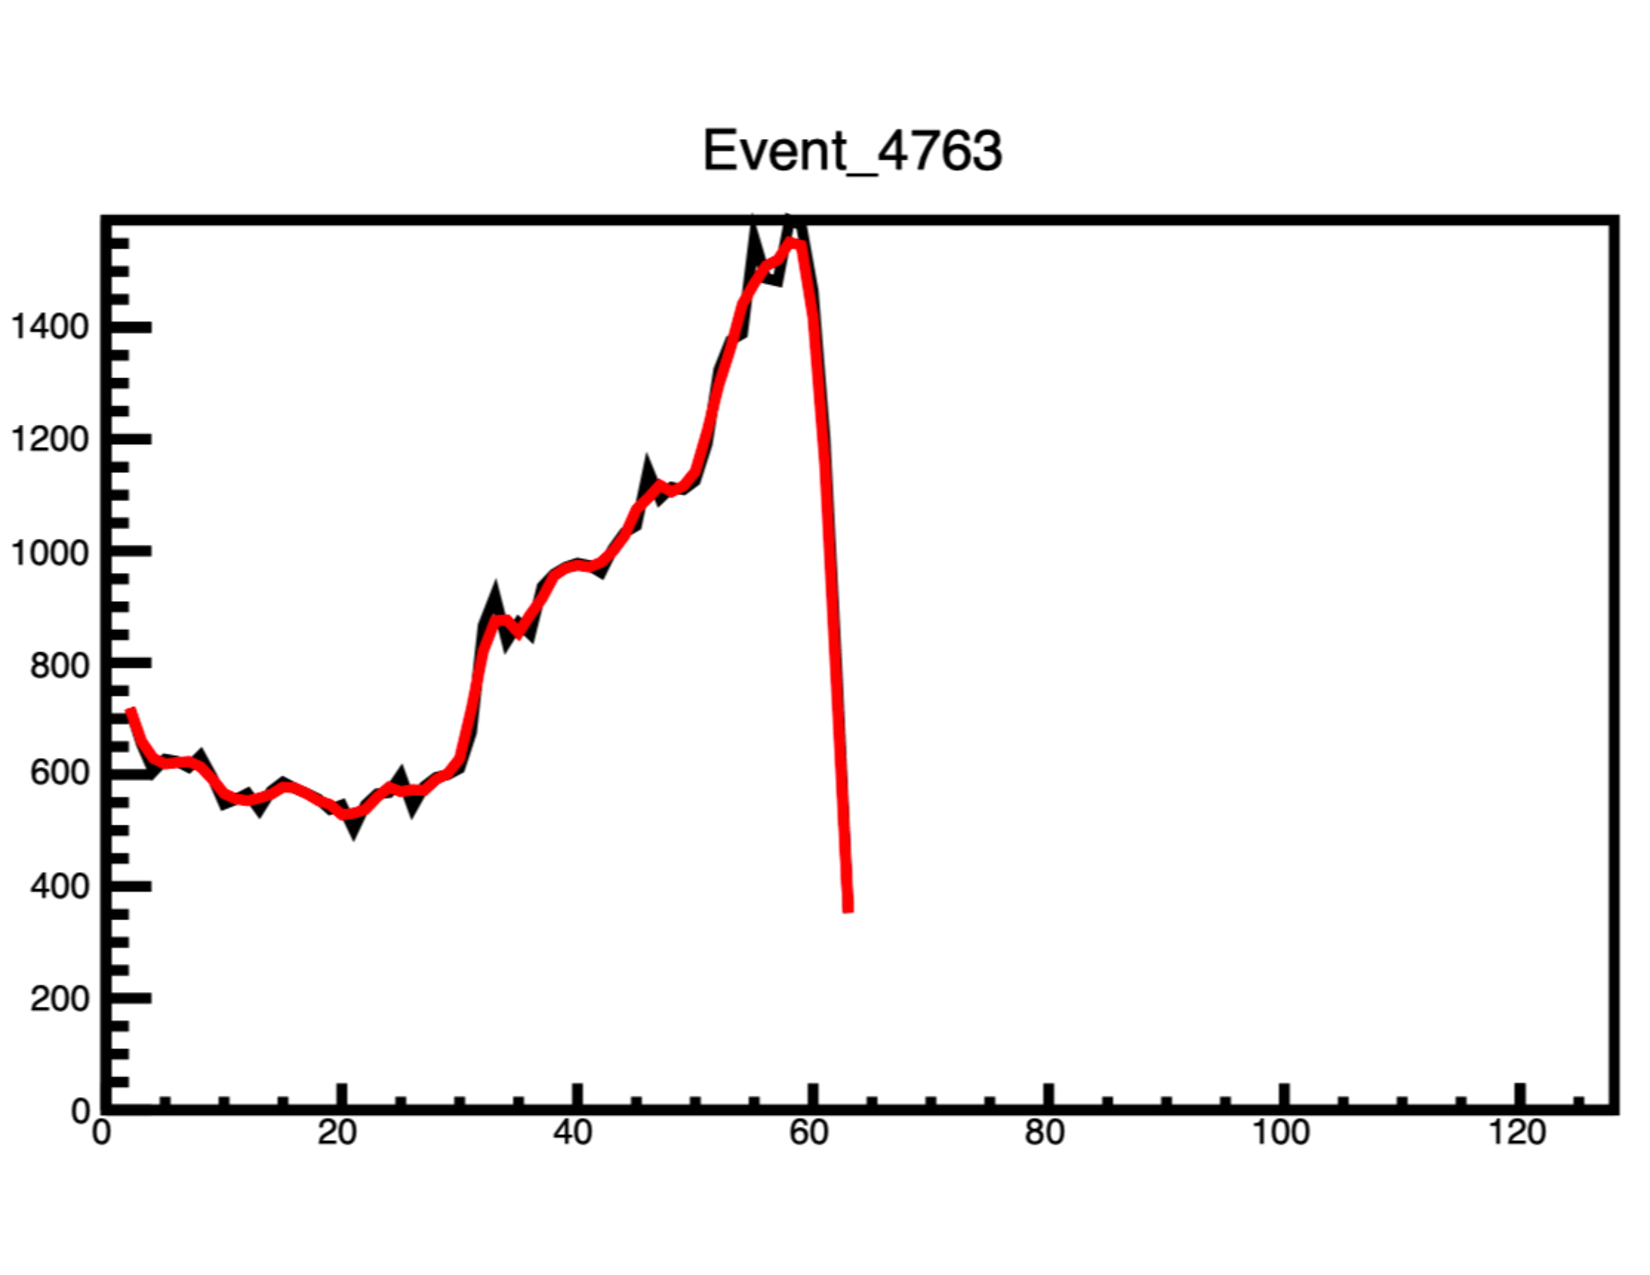
\includegraphics[width=\linewidth]{figures/9C_Center_Energy_2}
	\caption{Specific energy loss of the beam and heavy scattered recoil vs row number in Micromegas along the beam axis. Black lines are the raw energy values while the red curve is the running average. (Left) The vertex location is around row 20 while the maximum specific energy loss is around row 50. (Right) The vertex location is around row 30 while the maximum specific energy loss is around row 60.}
	\label{fig:9C_Center_Energy_Deposition}
\end{figure}

\begin{figure}[hbt!]
	\centering
    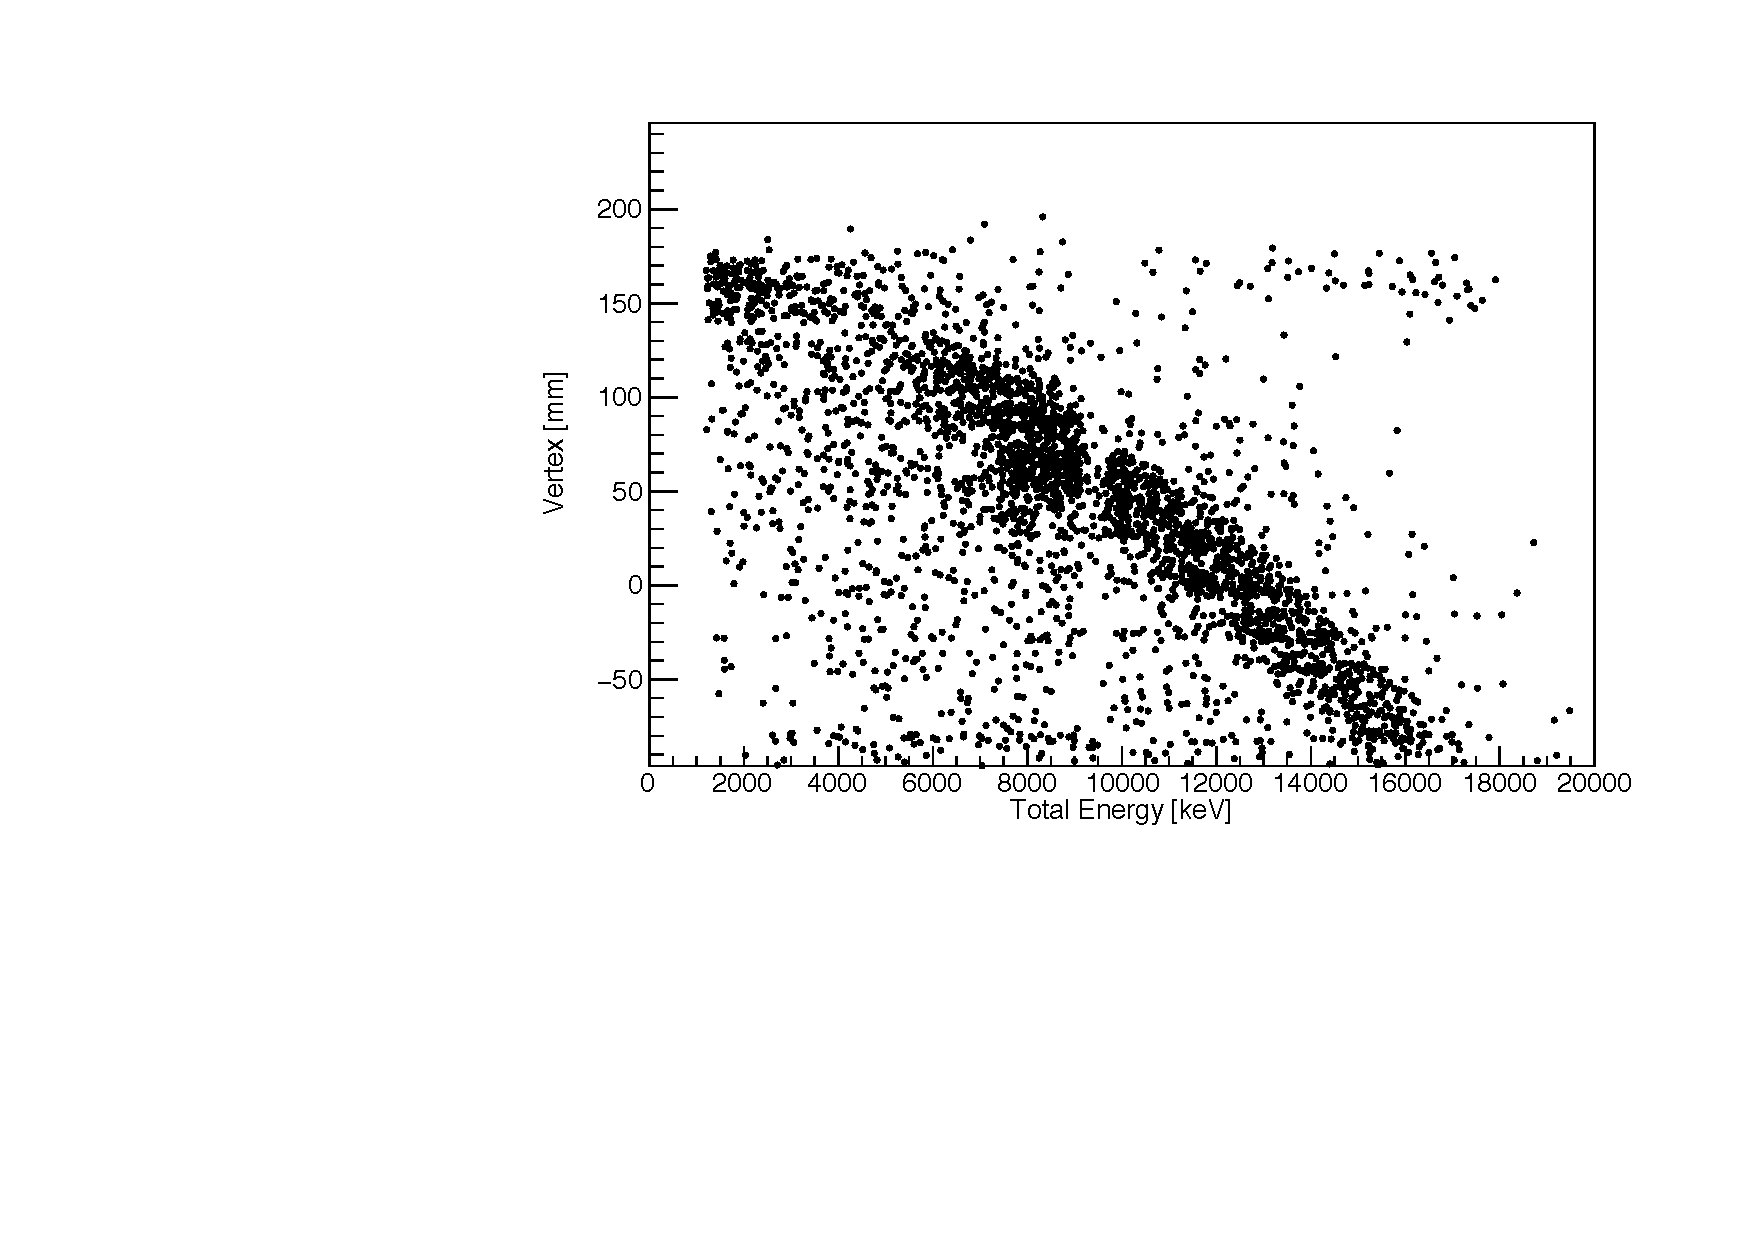
\includegraphics[width=0.5\textwidth]{figures/9C_VertexReconstructionRegion1}
    \caption{Vertex position vs total energy measured in the Si and CsI detectors for the central forward detectors.}
    \label{fig:9C_VertexReconstructionRegion1}
\end{figure}

\subsection{Vertex Reconstruction in the Side Regions}

Reconstructing the event tracks in the side regions is straightforward. After matching the strips and chains as discussed above, the tracks can then be analyzed using the Hough transform, and traced back to the beam axis to find the vertex location. For events where the vertex is over the Micromegas and the incoming beam is measured, the proton track is traced to the measured incoming beam track. For higher energy events, the beam information is not measured in the Micromegas detector and the proton track is traced back to the ``ideal'' beam axis. The measured vertex position vs total energy is shown in Fig. \ref{fig:9C_VertexReconstructionRegion3}. As in the case of the central region, elastically scattered events occur further away for high energy events and thus higher c.m. energy events.

\begin{figure}[hbt!]
	\centering
    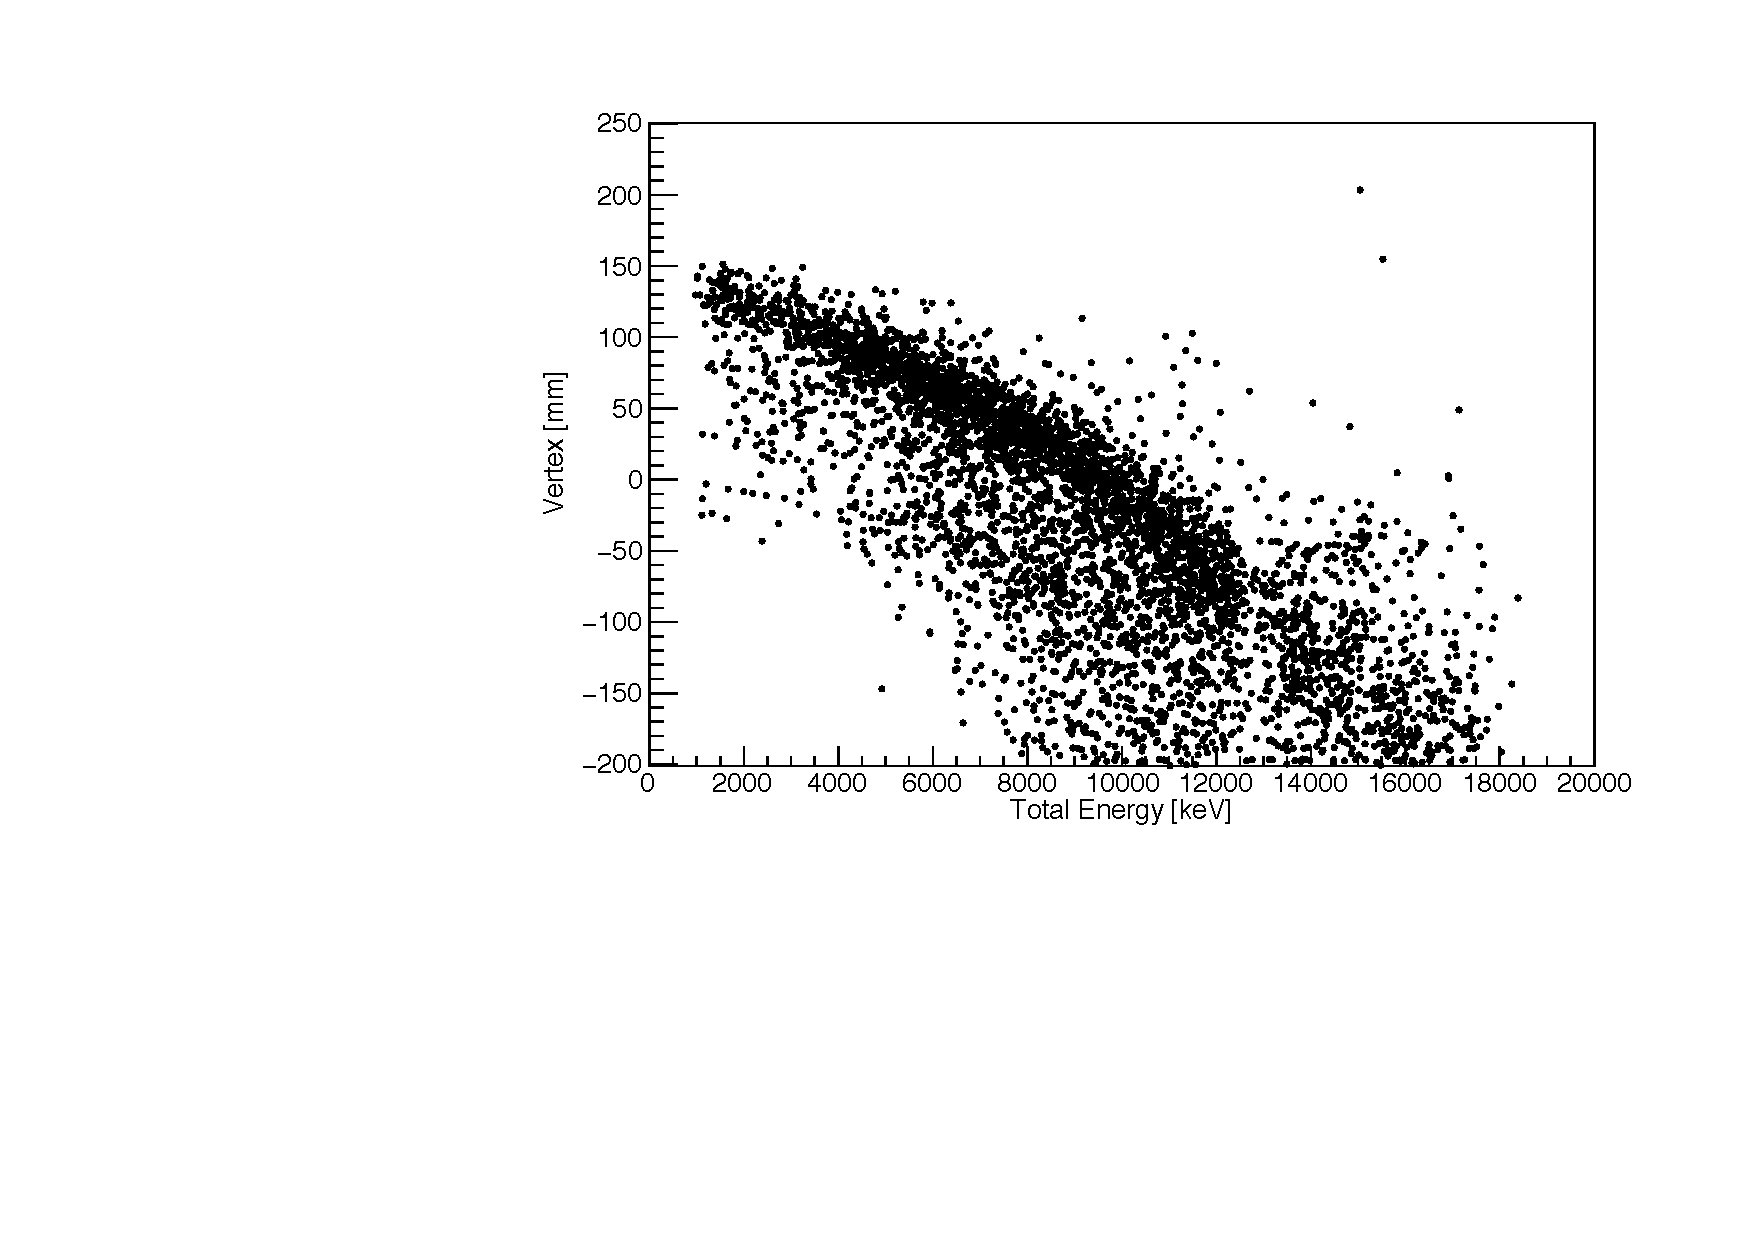
\includegraphics[width=0.5\textwidth]{figures/9C_VertexReconstructionRegion3}
    \caption{Vertex position vs total energy measured in the Si and CsI detectors for the outside forward detectors.}
    \label{fig:9C_VertexReconstructionRegion3}
\end{figure}


\section{Conclusion}

The new active target detector system - Texas Active Target (TexAT) - has been designed and constructed at the Cyclotron Institute at Texas A\&M University. The detector consists of the Time Projection Chamber (TPC) readout by highly segmented Micromegas detector that provides gas gains up to 10$^5$. The TPC is surrounded on five sided by the shell of Si detectors (700 - 1000 $\mu$m thick) backed by the CsI(Tl) scintillators of 40 mm thick, readout out by the Si pin-diodes. The detector was tested with $\alpha$-source first. The commissioning experiments with the stable $^{12}$C beam and the rare isotope $^8$B beam were performed. Parameters and properties of TexAT, the TexAT simulation package and simulation results and also track reconstruction procedures are described in this paper. Physics results of the first commissioning run, in which structure of exotic nucleus $^9$C was studied, are discussed in \cite{JHooker}.
 
\section*{Acknowledgements}

TexAT project  was supported by the U.S. Department of Energy, Office of Science, Office of
Nuclear Science, under Award No. DE-FG02-93ER40773 and by National Nuclear Security Administration through the Center for Excellence in Nuclear Training and University Based Research (CENTAUR) under grant number \#DE-NA0003841.
The author G.V.R. is also acknowledge the support of the Welch Foundation (Grant. No. A-1853).



%\bibliographystyle{unstr} 
\bibliography{NIM_TexAT}


\end{document}






	
	
	
	
	




